\PassOptionsToPackage{unicode}{hyperref}
\PassOptionsToPackage{hyphens}{url}
\PassOptionsToPackage{dvipsnames,svgnames,x11names}{xcolor}

\documentclass[10pt,letterpaper,openany,twoside]{report}

\usepackage{amsmath,amssymb}
\usepackage{iftex}
\ifPDFTeX
  \usepackage[T1]{fontenc}
  \usepackage[utf8]{inputenc}
  \usepackage{textcomp}
\else
  \usepackage{unicode-math}
  \defaultfontfeatures{Scale=MatchLowercase}
  \defaultfontfeatures[\rmfamily]{Ligatures=TeX,Scale=1}
  \setmainfont[]{DejaVu Serif}
  \setmonofont[]{DejaVu Sans Mono}
\fi
\ifPDFTeX
  \usepackage{lmodern}
\fi
\IfFileExists{upquote.sty}{\usepackage{upquote}}{}
\IfFileExists{microtype.sty}{%
  \usepackage[]{microtype}
  \UseMicrotypeSet[protrusion]{basicmath}
}{}

\usepackage{parskip}
\usepackage{xcolor}
\usepackage{colortbl}
\usepackage{graphicx}
\usepackage{tikz}
\usepackage[letterpaper,inner=0.88in,outer=0.82in,top=1.12in,bottom=1.08in,headheight=15pt,headsep=28pt,footskip=46pt]{geometry}
\usepackage{fancyhdr}
\usepackage{titlesec}
\usepackage{longtable,booktabs,array,hhline}
\usepackage{calc}
\usepackage{etoolbox}
\makeatletter
\patchcmd\longtable{\par}{\if@noskipsec\mbox{}\fi\par}{}{}
\makeatother
\IfFileExists{footnotehyper.sty}{\usepackage{footnotehyper}}{\usepackage{footnote}}
\makesavenoteenv{longtable}
\setlength{\emergencystretch}{3em}
\providecommand{\tightlist}{\setlength{\itemsep}{0pt}\setlength{\parskip}{0pt}}
\definecolor{APRSMarkerYellow}{RGB}{255,255,0}
\let\aprsorigtexttt\texttt
\newcommand{\aprsmarkerlit}[1]{\begingroup\setlength{\fboxsep}{1pt}\colorbox{APRSMarkerYellow}{\strut\aprsorigtexttt{#1}}\endgroup}
\newcommand{\lit}[1]{\aprsmarkerlit{#1}}
\renewcommand{\chaptername}{Chapitre}
\renewcommand{\contentsname}{Table des Matières}
\makeatletter
\renewcommand\tableofcontents{%
    \if@twocolumn
      \@restonecoltrue\onecolumn
    \else
      \@restonecolfalse
    \fi
    \clearpage
    \phantomsection
    \markboth{\contentsname}{\contentsname}%
    \vspace*{2.8em}%
    {\centering\sffamily\large\bfseries RÉFÉRENCE DU PROTOCOLE APRS\par}%
    \vspace{0.8em}%
    {\centering\sffamily\large\bfseries TABLE DES MATIÈRES\par}%
    \vspace{2.6em}%
    \@starttoc{toc}%
    \if@restonecol\twocolumn\fi
    }
\renewcommand*\l@chapter[2]{%
  \ifnum \c@tocdepth >\m@ne
    \addpenalty{-\@highpenalty}%
    \vskip 1.0em \@plus\p@
    \setlength\@tempdima{1.5em}%
    \begingroup
      \parindent \z@ \rightskip \@pnumwidth
      \parfillskip -\@pnumwidth
      \leavevmode \sffamily\bfseries
      \advance\leftskip\@tempdima
      \hskip -\leftskip
      #1\nobreak
      \leaders\hbox{$\m@th\mkern \@dotsep mu\hbox{.}\mkern \@dotsep mu$}\hfill
      \nobreak\hb@xt@\@pnumwidth{\hss #2}\par
      \penalty\@highpenalty
    \endgroup
  \fi}
\renewcommand*\l@section{\@dottedtocline{1}{1.5em}{0em}}
\renewcommand*\l@subsection{\@dottedtocline{2}{1.5em}{0em}}
\newcommand*\l@tocmain{\@dottedtocline{0}{0em}{0em}}
\def\@chapter[#1]#2{\ifnum \c@secnumdepth >\m@ne
                         \refstepcounter{chapter}%
                         \typeout{\@chapapp\space\thechapter.}%
                         \addcontentsline{toc}{chapter}%
                                   {\protect\numberline{\thechapter}#1}%
                    \else
                      \addcontentsline{toc}{chapter}{#1}%
                    \fi
                    \chaptermark{#2}%
                    \addtocontents{lof}{\protect\addvspace{10\p@}}%
                    \addtocontents{lot}{\protect\addvspace{10\p@}}%
                    \if@twocolumn
                      \@topnewpage[\@makechapterhead{#2}]%
                    \else
                      \@makechapterhead{#2}%
                      \@afterheading
                    \fi}
\makeatother
\setcounter{secnumdepth}{0}
\titleformat{\chapter}[block]
  {\normalfont\sffamily\large\bfseries}
  {\thechapter}{1em}{\MakeUppercase}
\titlespacing*{\chapter}{0pt}{2.8em}{2.6em}
\titleformat{\section}
  {\normalfont\sffamily\Large\bfseries}{\thesection}{1em}{}
\titleformat{\subsection}
  {\normalfont\sffamily\large\bfseries}{\thesubsection}{1em}{}
\titleformat{\subsubsection}
  {\normalfont\sffamily\normalsize\bfseries}{\thesubsubsection}{1em}{}
\titleformat{\paragraph}[runin]
  {\normalfont\sffamily\normalsize\bfseries}{\theparagraph}{1em}{}
\titleformat{\subparagraph}[runin]
  {\normalfont\sffamily\normalsize\bfseries}{\thesubparagraph}{1em}{}
\newenvironment{aprssideblock}[1]{%
  \begin{list}{}{%
    \setlength{\leftmargin}{0.275\textwidth}%
    \setlength{\rightmargin}{0pt}%
    \setlength{\itemsep}{0pt}%
    \setlength{\parsep}{0.65em}%
    \setlength{\topsep}{0.8em}%
  }%
  \item[]\leavevmode\llap{\parbox[t]{0.20\textwidth}{\raggedleft\sffamily\large\bfseries #1}\hspace{0.055\textwidth}}%
}{%
  \end{list}%
}
\newenvironment{aprsbodyblock}{%
  \begin{list}{}{%
    \setlength{\leftmargin}{0.275\textwidth}%
    \setlength{\rightmargin}{0pt}%
    \setlength{\itemsep}{0pt}%
    \setlength{\parsep}{0.65em}%
    \setlength{\topsep}{0.8em}%
  }%
  \item[]%
}{%
  \end{list}%
}
\ifLuaTeX
  \usepackage{selnolig}
\fi
\usepackage{bookmark}
\IfFileExists{xurl.sty}{\usepackage{xurl}}{}
\urlstyle{same}
\hypersetup{
  colorlinks=true,
  linkcolor={blue},
  filecolor={Maroon},
  citecolor={Blue},
  urlcolor={blue},
  pdftitle={Référence du protocole APRS 1.0 --- Traduction française},
  pdfauthor={APRS Working Group (trad.)},
  pdfsubject={APRS Protocol Reference 1.0.1},
  pdfcreator={LaTeX/lualatex}}

\pagestyle{fancy}
\fancyhf{}
\fancyhead[LE,RO]{\sffamily\bfseries\thepage}
\fancyhead[LO,RE]{\sffamily\bfseries\nouppercase{\leftmark}}
\newcommand{\APRSFooterLogo}{\raisebox{-0.42\height}{
\includegraphics[height=16pt]{figures/aprs-logo.png}}}
\fancyfoot[LO]{\APRSFooterLogo\hspace{0.6em}\sffamily\small\textbf{Référence du protocole APRS --- Version du protocole 1.0}}
\fancyfoot[RE]{\sffamily\small\textbf{Référence du protocole APRS --- Version du protocole 1.0}\hspace{0.6em}\APRSFooterLogo}
\fancyfoot[LE,RO]{\sffamily\scriptsize Document Version 1.0.1 : 29 août 2000}
\renewcommand{\headrulewidth}{0.4pt}
\renewcommand{\footrulewidth}{0.4pt}
\renewcommand{\chaptermark}[1]{\markboth{Chapitre \thechapter : #1}{}}
\assignpagestyle{\chapter}{fancy}
\fancypagestyle{plain}{%
  \fancyhf{}%
  \fancyfoot[C]{\small \thepage}%
  \renewcommand{\headrulewidth}{0pt}%
  \renewcommand{\footrulewidth}{0pt}%
}

\begin{document}

\begin{titlepage}
\thispagestyle{empty}
\sffamily
\vspace*{4.0em}
\hspace*{0.16\textwidth}%
\begin{minipage}{0.55\textwidth}
{\Large\bfseries AUTOMATIC POSITION\par}
{\Large\bfseries REPORTING SYSTEM\par}
\vspace{3.8em}
{\LARGE\bfseries APRS PROTOCOL\par}
{\LARGE\bfseries REFERENCE\par}
\vspace{1.2em}
{\large Protocol Version 1.0\par}
\vspace{4.0em}
\begin{tabular}{@{}r@{\hspace{1em}}l@{}}
Authors & The APRS Working Group \\
Document Version & Approved Version 1.0.1 \\
Filename & aprs101.pdf \\
Date of Issue & 29 August 2000 \\
Copyright & \copyright{}2000 APRS Working Group \\
 & All rights reserved \\
Technical Editor & Ian Wade, G3NRW \\
\end{tabular}
\end{minipage}
\end{titlepage}
\clearpage

\thispagestyle{empty}
\vspace*{1.0em}
\noindent{\sffamily\Large APRS Protocol Reference\par}
\noindent{\sffamily\large Protocol Version 1.0\par}

\vspace{1.2em}
\noindent by the APRS Working Group

\vspace{1.2em}
\noindent Edited by Ian Wade

\vspace{2.2em}
\noindent Published by

\noindent Tucson Amateur Packet Radio Corp

\noindent 8987--309 East Tanque Verde Road, \#337

\noindent Tucson

\noindent AZ 85749-9399

\noindent United States of America

\vspace{1.2em}
\noindent \url{http://www.tapr.org}

\vspace{1.8em}
\noindent ISBN 0-9644707-6-4

\vspace{1.2em}
\noindent TAPR Publication Number: 99-4

\vspace{2.0em}
\noindent Copyright \copyright{}2000 APRS Working Group

\noindent All rights reserved

\vspace{1.8em}
\noindent APRS\textregistered{} is a registered trademark of Bob Bruninga.

\noindent WinAPRS\texttrademark{}, MacAPRS\texttrademark{}, X-APRS\texttrademark{}, PalmAPRS\texttrademark{} and APRS/CE\texttrademark{}

\noindent are trademarks using the APRS\textregistered{} name, licensed from Bob Bruninga.

\vspace{1.8em}
\noindent This document may be copied for non-commercial purposes only, and must

\noindent include the above copyright statement and trademark statements in full.

\clearpage

\thispagestyle{empty}
\section*{Avant-propos}\label{avant-propos}
\markboth{Avant-propos}{Avant-propos}

Ce document de référence du protocole APRS marque la maturité du bébé de
WB4APR. Parti d'un concept simple --- un moyen de suivre la position
d'objets mobiles par packet radio --- les programmes utilisant le
protocole APRS sont devenus peut-être l'application packet radio la plus
populaire aujourd'hui. C'est aussi devenue l'une des plus complexes ; du
concept initial est né, et continue à croître, un système de
communication tactique d'une capacité considérable. Comme beaucoup de
projets amateurs, le protocole APRS a été conçu au fil de son
implémentation, et beaucoup de ses subtilités n'ont jamais été
documentées.

Jusqu'à maintenant. Cette spécification définit le protocole APRS sur
les ondes avec une précision et une clarté qui en font un modèle pour
les efforts futurs. Le travail accompli par les membres de l'APRS
Working Group, ainsi que par l'éditeur technique Ian Wade, G3NRW, doit
être reconnu comme une contribution majeure à l'art du packet radio.
Avec ce document disponible, aucun développeur n'a plus d'excuse pour
implémenter incorrectement le protocole APRS.

En tant que membre de l'APRS Working Group dont le rôle était
principalement celui d'observateur, j'ai été fasciné par les échanges
entre les auteurs APRS et l'éditeur technique au fur et à mesure que la
spécification prenait forme. Mettre sur papier des détails qui
existaient auparavant uniquement dans l'esprit des auteurs a mis au jour
des ambiguïtés, des conséquences non envisagées, et même des erreurs
dans ce que les auteurs croyaient savoir. Les discussions qui ont suivi
chaque brouillon, et les questions que Ian a posées pour lever les
incertitudes, ont donné à chacun une meilleure compréhension du
protocole. Je suis sûr que ce processus a déjà contribué à une meilleure
interopérabilité entre les applications APRS existantes.

Tous ceux qui ont suivi le développement de la spécification, depuis sa
première mention en avril 1999 jusqu'à la publication de cette Version
1.0 en août 2000, savent que le processus a pris beaucoup plus de temps
que prévu. Dans le même temps, ils ont vu le brouillon se transformer
d'un squelette en un livre substantiel de plus de 110 pages. Avec la
spécification maintenant en main, je pense que nous pouvons tous dire
que l'attente en valait la peine. Félicitations à l'APRS Working Group
et, en particulier, à G3NRW, pour une contribution majeure à la
littérature du packet radio.

\emph{John Ackermann, N8UR --- TAPR Vice President et Administrative
Chair du APRS Working Group --- août 2000}

\clearpage
\null
\thispagestyle{empty}
\clearpage

\hypersetup{linkcolor=blue}
\pagenumbering{roman}
\setcounter{tocdepth}{2}
\begingroup
\small
\tableofcontents
\endgroup
\clearpage
\null
\thispagestyle{empty}
\clearpage

\pagenumbering{arabic}

% Sections préliminaires (non numérotées)
\section*{PRÉAMBULE}\label{pruxe9ambule}
\markboth{Préambule}{Préambule}
\addcontentsline{toc}{tocmain}{PRÉAMBULE}

\phantomsection\addcontentsline{toc}{section}{APRS Working Group}
\begin{aprssideblock}{APRS Working\\Group}

L'APRS Working Group est une association non constituée en personne
morale dont les membres s'engagent à faire progresser l'usage et à
accroître la valeur des protocoles APRS en : (a) publiant et maintenant
une spécification formelle du protocole APRS ; (b) publiant des tests de
validation et d'autres outils permettant la conformité à la
spécification ; (c) soutenant un programme de certification APRS ; (d)
travaillant plus généralement à améliorer les capacités d'APRS au sein
de la communauté radio-amateur.

Bien que le Working Group puisse recevoir un soutien du TAPR et d'autres
organisations, il s'agit d'un corps indépendant, non affilié à aucune
organisation. Le groupe n'a pas de budget, ne collecte pas de
cotisations et ne possède aucun actif.

Membres actuels de l'APRS Working Group :

\begin{tabular}{@{}lll@{}}
John Ackermann, & N8UR & Administrative Chair \& représentant TAPR \\
Bob Bruninga, & WB4APR & Technical Chair, fondateur d'APRS \\
Brent Hildebrand, & KH2Z & Auteur de APRS+SA \\
Stan Horzepa, & WA1LOU & Secrétaire \\
Mike Musick, & N0QBF & Auteur de pocketAPRS \\
Keith Sproul, & WU2Z & Co-auteur de WinAPRS/MacAPRS/X-APRS \\
Mark Sproul, & KB2ICI & Co-auteur de WinAPRS/MacAPRS/X-APRS \\
\end{tabular}
\end{aprssideblock}

\phantomsection\addcontentsline{toc}{section}{Remerciements}
\begin{aprssideblock}{Remerciements}

Ce document est le résultat de contributions de nombreuses personnes. Il
reprend une grande partie du matériel produit par des membres
individuels du Working Group.

De plus, le document sur le format Mic-E par Alan Crosswell N2YGK et Ron
Parsons W5RKN a servi de point de départ utile pour expliquer les
complications de ce format.
\end{aprssideblock}

\phantomsection\addcontentsline{toc}{section}{Numéro de version du document}
\begin{aprssideblock}{Numéro de\\version du\\document}

À l'exception de la toute première version publique en brouillon de la
référence du protocole APRS, le numéro de version du document est un
numéro à 3 parties \texttt{P.p.D} (pour une version approuvée) ou à 4
parties \texttt{P.p.Dd} (pour un brouillon) :

\begin{itemize}
\tightlist
\item
  \texttt{P} : version majeure du protocole APRS
\item
  \texttt{p} : version mineure du protocole APRS
\item
  \texttt{D} : release du document
\item
  \texttt{d} : lettre du brouillon
\end{itemize}

Ainsi, par exemple :

\begin{itemize}
\tightlist
\item
  « 1.2.3 » = release 3 du document couvrant la version 1.2 du protocole
  APRS.
\item
  « 1.2.3c » = brouillon « c » de ce document.
\end{itemize}
\end{aprssideblock}

\phantomsection\addcontentsline{toc}{section}{Historique des versions}
\begin{aprssideblock}{Historique des\\versions}

Voir Annexe 7.
\end{aprssideblock}

\phantomsection\addcontentsline{toc}{section}{Conventions du document}
\begin{aprssideblock}{Conventions\\du document}

\begin{itemize}
\tightlist
\item
  Police \texttt{Courier} : caractères ASCII dans les données APRS.
\item
  \texttt{V} : caractère espace ASCII.
\item
  \texttt{…} (ellipse) : zéro ou plusieurs caractères.
\item
  \texttt{/\$} : symbole de la table de symboles primaire.
\item
  \texttt{\textbackslash{}\$} : symbole de la table de symboles
  alternative.
\item
  \texttt{0x} : hexadécimal (ex. \texttt{0x1d}).
\item
  Tous les indicatifs sont supposés avoir un SSID \texttt{-0} sauf
  mention contraire.
\item
  \lit{Marqueur jaune} (fond gris clair en impression papier) : signale un
  texte d'intérêt --- particulièrement utile pour mettre en évidence des
  caractères ASCII littéraux uniques (par exemple \lit{"}) tels
  qu'ils apparaissent dans les données APRS.
\item
  Zones grisées dans les diagrammes de format de paquet : champs
  optionnels.
\end{itemize}
\end{aprssideblock}

\phantomsection\addcontentsline{toc}{section}{Retour}
\begin{aprssideblock}{Retour}

Merci d'adresser retours et commentaires sur ce document à la liste de
diffusion TAPR \texttt{aprsspec}. Pour s'y inscrire, partir de
\url{http://www.tapr.org} puis suivre le chemin \emph{Special Interest
Groups → APRS Specification → Join APRS Spec Discussion List}.
\end{aprssideblock}

\section*{AVANT-PROPOS DES AUTEURS}\label{avant-propos-des-auteurs}
\markboth{Avant-propos des auteurs}{Avant-propos des auteurs}
\addcontentsline{toc}{tocmain}{AVANT-PROPOS DES AUTEURS}

\begin{aprsbodyblock}
Ce document de référence décrit ce que l'on appelle la Version 1.0 du
protocole APRS, et constitue essentiellement une description du
fonctionnement actuel d'APRS.

Il est destiné principalement au programmeur souhaitant développer des
applications compatibles APRS, mais intéressera aussi l'utilisateur
ordinaire qui veut en savoir plus sur ce qui se passe « sous le capot ».

Il n'est cependant pas destiné à être une spécification de programmation
ennuyeuse, pédante, de style RFC, à lire et à comprendre uniquement par
les Mr Spocks de ce monde. Nous avons inclus de nombreux éléments
d'information générale qui, bien que ne faisant pas strictement partie
de la description formelle du protocole, fournissent un contexte utile
sur la façon dont APRS est réellement utilisé sur les ondes, et sur la
manière dont il est implémenté dans les logiciels APRS. Nous espérons
que cela mettra APRS en perspective, rendra le document plus lisible, et
n'offensera pas trop les puristes.

Il est important de comprendre comment APRS est né, et de saisir la
philosophie de conception derrière lui. En particulier, nous croyons
fermement qu'APRS est, et doit rester, un système tactique léger ---
presque n'importe qui devrait pouvoir l'utiliser dans des situations
temporaires (urgences, travail mobile, veille météo) avec un minimum de
formation et d'équipement.

Ce document est le résultat des contributions de nombreuses personnes,
collationnées et retravaillées par l'APRS Working Group. Nos
remerciements sincères à tous ceux qui ont contribué à sa mise en forme
et à sa publication. Si vous découvrez des erreurs, des omissions ou des
affirmations trompeuses, faites-le nous savoir --- le meilleur moyen est
la liste de diffusion TAPR \texttt{aprsspec} sur
\href{http://www.tapr.org}{www.tapr.org}.

Enfin, des utilisateurs du monde entier proposent en permanence de
nouvelles idées et suggestions pour étendre et améliorer APRS. Nous les
accueillons volontiers. Là encore, le meilleur endroit pour en discuter
est la liste \texttt{aprsspec}.

\emph{L'APRS Working Group}

\emph{Août 2000}
\end{aprsbodyblock}

\phantomsection\addcontentsline{toc}{section}{Avertissement}
\begin{aprssideblock}{Avertissement}

Comme tout système de navigation, APRS n'est pas infaillible. Nul ne
devrait s'appuyer aveuglément sur APRS pour naviguer, ou dans des
situations de vie ou de mort. De même, cette spécification n'est pas
infaillible.

Les membres de l'APRS Working Group ont fait de leur mieux pour définir
le protocole APRS, mais cette description peut contenir des erreurs ou
des omissions. Il est très probable que toutes les implémentations APRS
n'appliqueront pas pleinement ou correctement cette spécification,
aujourd'hui ou à l'avenir.

Nous exhortons quiconque utilise ou écrit un programme implémentant
cette spécification à faire preuve de prudence et de bon sens. L'APRS
Working Group et l'éditeur de la spécification déclinent toute
responsabilité pour tout dommage aux personnes ou aux biens qui pourrait
résulter de l'utilisation de cette spécification ou d'un logiciel
l'implémentant.
\end{aprssideblock}

\clearpage

\section*{STRUCTURE DE CETTE
SPÉCIFICATION}\label{structure-de-cette-spuxe9cification}
\markboth{STRUCTURE DE CETTE SPÉCIFICATION}{STRUCTURE DE CETTE SPÉCIFICATION}
\addcontentsline{toc}{tocmain}{STRUCTURE DE CETTE SPÉCIFICATION}

\begin{aprsbodyblock}
Cette spécification décrit les exigences globales pour développer un
logiciel conforme à la Version 1.0 du protocole APRS. Le flux
d'information part de la trame AX.25 UI standard et descend
progressivement dans les détails, l'usage de chaque champ de la trame
étant exploré.

Une caractéristique clé de la spécification est l'inclusion de dizaines
d'exemples détaillés de paquets APRS typiques et des calculs
mathématiques associés.

Voici le plan des chapitres :

\begin{list}{}{\setlength{\leftmargin}{0pt}\setlength{\rightmargin}{0pt}\setlength{\itemindent}{0pt}\setlength{\labelwidth}{0pt}\setlength{\labelsep}{0pt}\setlength{\itemsep}{0.35em}\setlength{\parsep}{0pt}}
\item
  \textbf{Introduction à APRS} --- bref historique et résumé des
  principales caractéristiques.
\item
  \textbf{La philosophie de conception APRS} --- les fondamentaux
  d'APRS, avec son usage comme outil de communication tactique temps
  réel, le timing des transmissions APRS et l'usage du digipeating
  générique.
\item
  \textbf{APRS et AX.25} --- bref rappel sur la structure de la trame
  AX.25 UI, avec référence particulière aux usages spéciaux qu'APRS fait
  des champs Destination, Source et Information.
\item
  \textbf{Données APRS dans les champs Destination et Source AX.25} ---
  détails des indicatifs APRS génériques et des indicatifs qui
  spécifient des symboles d'affichage et des numéros de version. Résumé
  du stockage des données Mic-E dans le champ Destination, et de la
  spécification d'une icône via le SSID Source.
\item
  \textbf{Données APRS dans le champ Information AX.25} --- détails des
  principaux constituants des données APRS stockées dans le champ
  Information. Contient la table des Data Type Identifiers APRS et un
  résumé de tous les types de données possibles.
\item
  \textbf{Formats de temps et de position} --- timestamps, latitude,
  longitude, ambiguïté de position, Maidenhead, NMEA, altitude.
\item
  \textbf{Extensions de données APRS} --- extensions optionnelles pour
  course/vitesse de la station, vitesse/direction du vent,
  puissance/hauteur/gain, portée radio pré-calculée, force de signal DF,
  descripteur d'objet zone.
\item
  \textbf{Formats de rapports de position et DF} --- détails complets de
  ces formats.
\item
  \textbf{Formats compressés de rapport de position} --- comment la
  position d'une station et les extensions APRS sont compressées en
  paquets très courts.
\item
  \textbf{Format de données Mic-E} --- encodage Mic-E de la lat/long,
  altitude, course, vitesse, code message Mic-E, données de télémétrie
  et chemin de digipeater APRS dans les champs Destination et
  Information de la trame AX.25.
\item
  \textbf{Rapports d'objets et d'éléments} --- comment configurer des
  objets et éléments APRS, et détails de l'encodage des Area Objects
  (cercles, lignes, ellipses, etc.).
\item
  \textbf{Rapports météo} --- détails complets pour les stations météo
  autonomes (sans position) et pour les rapports contenant une
  information de position. Détail du format Storm Data.
\item
  \textbf{Données de télémétrie} --- description du format MIM/KPC-3+,
  avec informations pour adapter l'interprétation des données brutes aux
  circonstances individuelles.
\item
  \textbf{Messages, bulletins et annonces} --- format complet.
\item
  \textbf{Capacités, requêtes et réponses de station} --- dix types de
  requêtes et les réponses attendues.
\item
  \textbf{Rapports de statut} --- format des messages de statut général,
  plus les cas particuliers d'usage pour véhiculer beam
  heading/puissance en meteor scatter et locator Maidenhead.
\item
  \textbf{Tunneling réseau} --- usage du Source Path Header pour
  tunneliser des paquets APRS à travers des réseaux tiers qui ne
  comprennent pas les adresses AX.25, et usage du Data Type Identifier
  tiers.
\item
  \textbf{Format défini par l'utilisateur} --- APRS permet aux
  utilisateurs de définir leurs propres formats à des fins
  particulières. Ce chapitre explique comment faire.
\item
  \textbf{Autres paquets} --- énoncé général sur la façon dont APRS doit
  traiter tout autre type de paquet non couvert par cette spécification.
\item
  \textbf{Symboles APRS} --- comment spécifier symboles et overlays dans
  les rapports de position et dans les indicatifs de destination GPS
  génériques.
\item
  \textbf{Formats de données APRS} --- annexe rassemblant tous les
  formats pour référence.
\item
  \textbf{Tables de symboles APRS} --- liste complète des symboles des
  tables Primary et Alternate.
\item
  \textbf{Table des codes ASCII} --- code ASCII complet, décimal et
  hexadécimal (le décimal est nécessaire pour les calculs de lat/long
  compressées et d'altitude), avec les codes hex des caractères ASCII
  bit-shiftés dans les adresses AX.25 (utile pour décoder Mic-E et pour
  le monitoring de paquets on-air).
\item
  \textbf{Glossaire} --- référence tout-en-un des nombreux termes
  spécifiques APRS.
\item
  \textbf{Références} --- pointeurs vers d'autres documents pertinents.
\end{list}
\end{aprsbodyblock}

\begin{center}\rule{0.5\linewidth}{0.5pt}\end{center}


% Chapitres 1 à 20 (numérotés)
\chapter[INTRODUCTION À APRS]{Introduction à APRS}\label{introduction-uxe0-aprs}

\phantomsection\addcontentsline{toc}{section}{Qu'est-ce qu'APRS ?}
\begin{aprssideblock}{Qu'est-ce\\qu'APRS ?}
APRS est l'abréviation d'\emph{Automatic Position Reporting System},
conçu par Bob Bruninga WB4APR et présenté par lui à la conférence
TAPR/ARRL Digital Communications de 1992.

Fondamentalement, APRS est un protocole de communication packet destiné
à diffuser en temps réel des données vivantes à tous les nœuds d'un
réseau. Sa fonctionnalité la plus visible est la combinaison du packet
radio avec le réseau satellite GPS, permettant aux radioamateurs
d'afficher automatiquement sur une carte PC la position de stations et
d'autres objets. D'autres fonctions non directement liées au reporting
de position sont supportées : stations météo, radiogoniométrie et
messagerie.

APRS diffère du packet classique à plusieurs égards :

\begin{itemize}
\tightlist
\item
  Cartes et affichages de données, pour la localisation
  véhicules/personnels et le reporting météo en temps réel.
\item
  Communications \emph{one-to-many}, chacun étant mis à jour
  immédiatement.
\item
  Digipeating générique avec alias d'indicatifs bien connus --- pas
  besoin de connaître la topologie du réseau à l'avance.
\item
  Digipeating intelligent avec substitution d'indicatif pour réduire le
  flooding.
\item
  Sur trames AX.25 UI, supporte la messagerie bidirectionnelle et la
  diffusion de bulletins/annonces.
\item
  Communications avec les radios Kenwood TH-D7 et TM-D700 (TNC et
  firmware APRS intégrés).
\end{itemize}

Le packet radio conventionnel n'est vraiment utile que pour transporter
du trafic messagerie en masse d'un point à un autre, et a
traditionnellement été difficile à appliquer à des événements temps réel
où l'information a une durée de vie très courte. APRS transforme le
packet radio en un système de communication et d'affichage tactique
temps réel pour urgences et missions de service public.

APRS fournit une connectivité universelle entre toutes les stations,
sans la complexité, les délais et les limites d'un réseau à connexion.
N'importe quel nombre de stations peut échanger des données comme le
feraient des utilisateurs voix sur un net vocal. Toute station qui a
quelque chose à partager l'envoie, toutes les stations le reçoivent et
le journalisent.

APRS reconnaît qu'un des besoins temps réel les plus importants lors
d'un événement ou d'une urgence est le suivi d'actifs clés. Où est le
leader du marathon ? Où sont les véhicules de secours ? Quelle météo en
tel point ? Où sont les lignes électriques tombées ? Où est la tête du
défilé ? Où est la caméra ATV mobile ? Où est l'orage ?

Pour ces questions, APRS fournit un système complet de localisation
automatique et de reporting de statut. Il peut fonctionner sur n'importe
quel système radio bidirectionnel --- amateur, marine, cellulaire. Il
existe même un réseau international de suivi APRS en direct sur
Internet.
\end{aprssideblock}

\phantomsection\addcontentsline{toc}{section}{Fonctionnalités APRS}
\begin{aprssideblock}{Fonctionnalités\\APRS}
APRS tourne sur la plupart des plateformes : DOS, Windows 3.x, Windows
95/98, MacOS, Linux, Palm. La plupart des implémentations supportent les
principales fonctions :

\begin{itemize}
\tightlist
\item
  \textbf{Cartes} --- positions des stations APRS tracées en temps réel,
  échelle de quelques centaines de mètres à monde entier. Les stations
  reportant course et vitesse sont extrapolées à leur position actuelle
  par dead-reckoning. Bases de données superposables : digipeaters APRS,
  sites du National Weather Service US, magasins de matériel radio. Zoom
  possible sur n'importe quel point du globe.
\item
  \textbf{Reporting de station météo} --- affichage automatique
  d'informations météo distantes à l'écran.
\item
  \textbf{Reporting DX Cluster} --- outil idéal pour l'utilisateur de DX
  cluster. Quelques stations APRS connectées à des clusters peuvent
  relayer les infos de station DX à beaucoup d'autres stations locales,
  réduisant la charge packet globale sur les clusters.
\item
  \textbf{Accès Internet} --- Internet peut être utilisé de manière
  transparente pour interconnecter des réseaux radio locaux partout dans
  le monde. On peut se connecter en telnet à des serveurs APRS Internet
  et voir en direct des centaines de stations du monde entier. Tout le
  monde peut alimenter le serveur avec ses paquets locaux, tout le monde
  partout peut les voir.
\item
  \textbf{Messages} --- messages bidirectionnels avec accusé de
  réception. Chaque message entrant alerte l'utilisateur et reste
  affiché jusqu'à effacement manuel.
\item
  \textbf{Bulletins et annonces} --- adressés à tous. Les bulletins sont
  envoyés quelques fois par heure pendant quelques heures ; les annonces
  moins fréquemment mais peut-être sur plusieurs jours.
\item
  \textbf{Suivi de stations fixes} --- en plus du suivi automatique des
  stations mobiles GPS/LORAN, APRS suit aussi les rapports manuels ou
  par grid square.
\item
  \textbf{Objets} --- n'importe quel utilisateur peut placer un Object
  APRS sur sa carte, et en quelques secondes cet objet apparaît sur tous
  les autres écrans. Utile pour tracker des ressources non équipées de
  trackers : un seul opérateur, en écoutant la voix, tient à jour les
  positions ; toutes les autres stations en profitent.
\end{itemize}
\end{aprssideblock}


\chapter[LA PHILOSOPHIE DE CONCEPTION APRS]{La philosophie de conception
APRS}\label{la-philosophie-de-conception-aprs}

\begin{aprssideblock}{Net Cycle Time}
\phantomsection\addcontentsline{toc}{section}{Net Cycle Time}\label{net-cycle-time}

APRS est avant tout un outil de communication tactique temps réel,
destiné à faciliter le flux d'information lors d'événements spéciaux,
urgences, Skywarn, centre d'opérations d'urgence, ou simplement usage
terrain sous stress. Mais comme dans le monde réel, 99 \% du temps il
fonctionne en routine, en attente de l'événement sérieux improbable.

Toute évolution d'APRS doit préserver sa capacité à fonctionner
localement sous stress. Détails de cette philosophie :

\begin{enumerate}
\def\labelenumi{\arabic{enumi}.}
\item
  APRS utilise le concept de « net cycle time » --- durée dans laquelle
  un utilisateur doit avoir entendu (au moins une fois) toutes les
  stations APRS à portée, pour obtenir une image plus ou moins complète
  de l'activité. Le net cycle time varie avec les conditions locales et
  le nombre de digipeaters traversés.
\item
  Objectif : 10 minutes de net cycle time en usage local. En 10 minutes
  après l'arrivée sur les lieux, on doit avoir capturé toute la
  situation tactique.
\item
  Toutes les stations, même fixes, doivent beaconer leur position au
  rythme du net cycle time. En situation de stress, les stations vont et
  viennent en permanence. Les rapports de position montrent où elles
  sont sans qu'on ait à demander, et signalent qu'elles sont toujours
  actives.
\item
  On ne peut pas supposer que tous les utilisateurs APRS répondant à un
  événement comprennent les ramifications d'APRS et les statistiques du
  canal --- les réglages utilisateurs ne suffisent pas pour éviter de
  tuer un réseau sous stress. Pour anticiper une saturation, APRS ajuste
  automatiquement son net cycle time selon le nombre de digipeaters dans
  le chemin UNPROTO :

  \begin{itemize}
  \tightlist
  \item
    Opération directe (aucun digipeater) : 10 minutes (probablement un
    événement).
  \item
    1 hop : 10 minutes (probablement un événement).
  \item
    2 hops : 20 minutes.
  \item
    3 hops ou plus : 30 minutes.
  \end{itemize}
\item
  Comme quasiment toutes les stations fixes règlent leur chemin sur 3
  digis ou plus, le net cycle time par défaut en usage quotidien routine
  est de 30 minutes. Standard universel : allume la radio et APRS, ne
  fais rien d'autre, en 30 minutes tu as l'image complète de toutes les
  stations APRS à portée.
\item
  Comme la connaissance de la localisation des digipeaters est
  fondamentale, les digipeaters devraient utiliser plusieurs commandes
  de beacon pour transmettre à différents rythmes et sur différents
  chemins --- par ex. 10 min localement, 30 min via 3 digis (et d'autres
  selon besoin).
\item
  Si le net cycle time est trop long, les utilisateurs seront tentés
  d'envoyer des requêtes de stations, ce qui augmentera inutilement le
  trafic. Extrêmes recommandés : 10 et 30 minutes --- ça donne aux
  concepteurs de réseau les hypothèses de charge canal nécessaires à une
  bonne ingénierie.
\end{enumerate}
\end{aprssideblock}

\begin{aprssideblock}{Packet Timing}
\phantomsection\addcontentsline{toc}{section}{Packet Timing}\label{packet-timing}

Les paquets APRS sont sans erreur (grâce à la FCS AX.25) mais sans
livraison garantie. APRS transmet donc l'information de façon
redondante. Pour assurer une livraison rapide des données nouvelles ou
changeantes, et préserver la capacité canal en réduisant les
interférences avec les données anciennes, APRS doit transmettre les
données récentes plus souvent que les anciennes.

Plusieurs algorithmes en usage :

\begin{itemize}
\tightlist
\item
  \textbf{Decay Algorithm} --- transmettre un nouveau paquet une fois,
  puis n secondes plus tard. Doubler n à chaque nouvelle transmission.
  Quand n atteint le net cycle time, rester à ce rythme. D'autres
  facteurs que « doubler » sont possibles selon le contexte.
\item
  \textbf{Fixed Rate} --- transmettre une fois, puis n secondes plus
  tard. Répéter x fois puis s'arrêter.
\item
  \textbf{Message-on-Heard} --- transmettre selon l'un des algorithmes
  ci-dessus. Si le paquet est toujours valide et n'a pas été acquitté,
  et si le net cycle time est atteint, le destinataire est probablement
  absent. Cependant si un paquet du destinataire est ensuite entendu,
  réessayer une fois de transmettre.
\item
  \textbf{Time-Out} --- période au-delà de laquelle on peut
  raisonnablement considérer qu'une station n'existe plus ou est off-air
  si aucun paquet n'a été entendu. Défaut nominal : 2 heures. Ce
  time-out n'est pas utilisé dans les algorithmes de transmission mais
  sert à décider quand cesser d'afficher une station comme « active ».
  Sur HF, les signaux vont et viennent --- décisions plus flexibles.
\end{itemize}
\end{aprssideblock}

\begin{aprssideblock}{Digipeating\\générique}
\phantomsection\addcontentsline{toc}{section}{Digipeating générique}\label{digipeating-guxe9nuxe9rique}

La puissance d'APRS sur le terrain vient de l'usage du digipeating
générique : les paquets se propagent sans connaissance a priori du
réseau. Six techniques ont évolué depuis 1992 :

\begin{enumerate}
\def\labelenumi{\arabic{enumi}.}
\tightlist
\item
  \textbf{RELAY} --- tout TNC APRS VHF est supposé avoir l'alias
  \texttt{RELAY}, utilisable comme digipeater par n'importe qui.
\item
  \textbf{ECHO} --- les stations HF utilisent l'alias \texttt{ECHO}
  comme alternative à \texttt{RELAY}. Attention à la propagation HF qui
  peut causer des interférences sur une vaste zone --- usage
  parcimonieux.
\item
  \textbf{WIDE} --- tout digipeater en hauteur est supposé avoir l'alias
  \texttt{WIDE} pour couvrir plus loin.
\item
  \textbf{TRACE} --- tout digipeater en hauteur pratiquant la
  substitution d'indicatif est supposé avoir l'alias \texttt{TRACE}. Ces
  digipeaters s'auto-identifient dans les paquets qu'ils digipeatent en
  substituant leur indicatif à \texttt{RELAY}, \texttt{WIDE} ou
  \texttt{TRACE}.
\item
  \textbf{WIDEn-N} --- un digipeater supportant WIDEn-N digipeatera tout
  paquet WIDEn-N « nouveau » et décrémentera le SSID jusqu'à ce qu'il
  atteigne \texttt{-0}. Le digipeater garde une copie ou un checksum et
  ne re-digipeatera pas le même paquet dans un intervalle typique de 28
  s. Réduit considérablement les doublons dans les zones où plusieurs
  digipeaters s'entendent.
\item
  \textbf{GATE} --- indicatif générique pour les gateways HF-VHF. Tout
  paquet entendu en HF via \texttt{GATE} est digipeaté localement en
  VHF. Les réseaux locaux gardent un œil sur l'échelle
  nationale/internationale.
\end{enumerate}
\end{aprssideblock}

\begin{aprssideblock}{Vues\\cartographiques}
\phantomsection\addcontentsline{toc}{section}{Communiquer des vues cartographiques sans ambiguïté}\label{communiquer-des-vues-cartographiques-sans-ambiguuxeftuxe9}

APRS est un système géographique tactique. Pour maximiser son efficacité
opérationnelle et minimiser la confusion entre opérateurs, il faut une
manière non ambiguë de communiquer la « localisation » et la « taille »
(aire de couverture) d'une vue.

La convention APRS : référence à un \emph{centre} et à un \emph{range}
qui spécifient le centre géographique et le rayon approximatif d'un
cercle inscrit dans la vue, indépendant de l'aspect ratio. Ce rayon (en
milles nautiques, milles terrestres ou km) est le « range scale ». Base
commune simple pour décrire n'importe quelle vue à d'autres, quel que
soit le médium ou le programme.
\end{aprssideblock}

\chapter[APRS ET AX.25]{APRS et AX.25}\label{aprs-et-ax.25}

\begin{aprssideblock}{Protocoles}
\phantomsection\addcontentsline{toc}{section}{Protocoles}\label{protocoles}

Au niveau lien, APRS utilise le protocole AX.25 (voir référence
\emph{Amateur Packet-Radio Link-Layer Protocol} en annexe 6),
exclusivement en trames UI (Unnumbered Information). Cela signifie
qu'APRS tourne en mode sans connexion : les trames sont émises sans
attendre de réponse, et la réception à l'autre bout n'est pas garantie.

À un niveau plus haut, APRS supporte un protocole de messagerie
permettant aux utilisateurs d'envoyer des messages courts (une ligne) à
des stations nommées, avec accusé de réception attendu.
\end{aprssideblock}

\begin{aprssideblock}{La trame\\AX.25}
\phantomsection\addcontentsline{toc}{section}{La trame AX.25}\label{la-trame-ax.25}

Toutes les transmissions APRS utilisent des trames AX.25 UI avec 9
champs :
\end{aprssideblock}

\begin{center}
{\scriptsize
\setlength{\tabcolsep}{2pt}
\renewcommand{\arraystretch}{1.45}
\makebox[0.11\textwidth][r]{\vphantom{\begin{tabular}{|c|}\hline X\\\hline X\\\hline X\\\hline\end{tabular}}}%
\begin{tabular*}{0.89\textwidth}{@{\extracolsep{\fill}}|c|c|c|c|c|c|c|c|c|}
\multicolumn{9}{|>{\columncolor{black}}l|}{\textcolor{white}{\bfseries AX.25 UI-FRAME FORMAT}}\\
\hline
\bfseries Flag & \bfseries Destination & \bfseries Source & \bfseries Digipeater & \bfseries Control & \bfseries Protocol & \bfseries INFORMATION & \bfseries FCS & \bfseries Flag \\
               & \bfseries Address     & \bfseries Address& \bfseries Addresses  & \bfseries Field   & \bfseries ID       & \bfseries FIELD       &              &              \\
               &                       &                  & \bfseries (0--8)     & \bfseries (UI)    &                    &                       &              &              \\
\hline
\makebox[0pt][r]{Octets :\hspace{1.6em}}1 & 7 & 7 & 0--56 & 1 & 1 & 1--256 & 2 & 1 \\
\hline
\end{tabular*}
}
\end{center}

\begin{aprssideblock}{}
\begin{itemize}
\tightlist
\item
  \textbf{Flag} --- bit sequence \texttt{0x7e} séparant chaque trame, à
  chaque extrémité.
\item
  \textbf{Destination Address} --- peut contenir un indicatif de
  destination APRS ou des données APRS encodées pour respecter le format
  AX.25 standard (6 alphanumériques + SSID). SSID non nul = chemin
  digipeater APRS générique.
\item
  \textbf{Source Address} --- indicatif et SSID de la station émettrice.
  Dans certains cas, un SSID non nul spécifie un code de symbole
  d'affichage.
\item
  \textbf{Digipeater Addresses} --- 0 à 8 indicatifs de digipeaters.
  Peuvent être remplacés par un chemin APRS générique spécifié dans le
  SSID de destination.
\item
  \textbf{Control Field} --- mis à \texttt{0x03} (UI-frame).
\item
  \textbf{Protocol ID} --- mis à \texttt{0xf0} (pas de protocole de
  couche 3).
\item
  \textbf{Information Field} --- données APRS. Le premier caractère est
  le Data Type Identifier qui précise la nature du contenu.
\item
  \textbf{FCS} --- Frame Check Sequence sur 16 bits pour intégrité de la
  trame.
\end{itemize}
\end{aprssideblock}

\titlespacing*{\chapter}{0pt}{-1em}{2.6em}
\chapter[DONNÉES APRS DANS LES CHAMPS DESTINATION ET SOURCE AX.25]{Données APRS dans les champs Destination et Source
AX.25}\label{donnuxe9es-aprs-dans-les-champs-destination-et-source-ax.25}
\titlespacing*{\chapter}{0pt}{2.8em}{2.6em}

\begin{aprssideblock}{Le champ\\Destination Address\\AX.25}
\phantomsection\addcontentsline{toc}{section}{Le champ Destination Address AX.25}\label{le-champ-destination-address-ax.25}
Le champ Destination Address AX.25 peut contenir 6 types d'information APRS :

\begin{itemize}
\tightlist
\item
  Une adresse APRS générique.
\item
  Une adresse APRS générique avec un symbole.
\item
  Un numéro de version de logiciel APRS.
\item
  Des données encodées Mic-E.
\item
  Un Maidenhead Grid Locator (obsolète).
\item
  Une adresse Alternate Net (ALTNET).
\end{itemize}

Dans chacun de ces cas, le SSID de Destination Address peut spécifier un chemin
digipeater APRS générique.
\end{aprssideblock}

\begin{aprssideblock}{Adresses génériques\\de destination APRS}
\phantomsection\addcontentsline{toc}{section}{Adresses génériques de destination APRS}\label{adresses-guxe9nuxe9riques-de-destination-aprs}
APRS utilise les adresses génériques de type beacon suivantes :

\begin{center}
\ttfamily
\begin{tabular}{lllllll}
\lit{AIR}*† & \lit{CQ}* & \lit{DX}* & \lit{MAIL}* & \lit{RTCM}* & \lit{SYM}* & \lit{WX}* \\
\lit{ALL}* & \lit{DF}* & \lit{GPS}* & \lit{MICE}* & \lit{SKY}* & \lit{TEL}* & \lit{ZIP}*† \\
\lit{AP}* & \lit{DGPS}* & \lit{ID}* & \lit{QST}* & \lit{SPACE}* & \lit{TEST}* & \\
\lit{BEACON} & \lit{DRILL}* & \lit{JAVA}* & \lit{QTH}* & \lit{SPC}* & \lit{TLM}* & \\
\end{tabular}
\end{center}

L'astérisque est un joker permettant d'étendre l'adresse jusqu'à un total de
6 caractères alphanumériques. Ainsi, par exemple, \texttt{WX1}, \texttt{WX12}
et \texttt{WX12CD} sont toutes des adresses de destination APRS valides.

† Les adresses {\ttfamily \lit{AIR}*} et {\ttfamily \lit{ZIP}*} sont en cours
d'abandon, mais sont actuellement nécessaires pour assurer la compatibilité
avec les versions antérieures.

Toutes ces adresses ont un SSID de \texttt{-0}. Les SSID non nuls sont
réservés au digipeating APRS générique.

Ces adresses sont copiées par tous. Tous les logiciels APRS doivent accepter
les paquets comportant ces adresses de destination.

L'adresse \lit{GPS}, c'est-à-dire l'adresse exacte à 3 lettres \lit{GPS} et
non {\ttfamily \lit{GPS}*}, est spécifiquement destinée aux trackers qui
envoient des positions latitude/longitude par l'intermédiaire de digipeaters
capables de convertir les positions au format de données compressées.

Les adresses \lit{DGPS} et \lit{RTCM} sont utilisées par les stations de
correction GPS différentielle. La plupart des logiciels n'exploitent pas les
paquets utilisant ces adresses, si ce n'est pour les transmettre à un
récepteur GPS connecté.

L'adresse \lit{SKY} est utilisée par les stations Skywarn.

Les paquets adressés à {\ttfamily \lit{SPC}L} sont destinés aux événements
spéciaux. Les logiciels APRS peuvent afficher ces paquets à l'exclusion de
tous les autres, afin de réduire à l'écran l'encombrement produit par les
autres stations ne participant pas à l'événement spécial.

Les adresses \lit{TEL} et \lit{TLM} sont utilisées par les stations de
télémétrie.
\end{aprssideblock}

\begin{aprssideblock}{Adresse générique\\avec symbole}
\phantomsection\addcontentsline{toc}{section}{Adresse générique avec symbole}\label{adresse-guxe9nuxe9rique-avec-symbole}
APRS utilise plusieurs des adresses génériques énumérées ci-dessus d'une
manière particulière, afin de spécifier non seulement une adresse, mais aussi
un symbole d'affichage. Ces adresses particulières sont
{\ttfamily \lit{GPS}xyz}, {\ttfamily \lit{GPS}Cnn},
{\ttfamily \lit{GPS}Enn}, {\ttfamily \lit{SPC}xyz} et
{\ttfamily \lit{SYM}xyz}. Elles sont destinées aux cas dans lesquels il est
impossible d'inclure le symbole dans le champ Information AX.25.

Les adresses {\ttfamily \lit{GPS}…} ci-dessus sont destinées à un usage
général.

Les adresses {\ttfamily \lit{SPC}…} sont destinées aux événements spéciaux.

Les adresses {\ttfamily \lit{SYM}…} sont réservées à un usage futur.

Les caractères \texttt{xy} et \texttt{nn} désignent des entrées des tables de
symboles APRS. Le caractère \texttt{z} spécifie un overlay de symbole. Voir le
chapitre 20 : Symboles APRS et l'annexe 2 pour plus d'informations.
\end{aprssideblock}

\begin{aprssideblock}{Numéro de version\\du logiciel APRS}
\phantomsection\addcontentsline{toc}{section}{Numéro de version du logiciel APRS}\label{numuxe9ro-de-version-de-logiciel-aprs}
Le champ Destination Address AX.25 peut contenir le numéro de version du
logiciel APRS exécuté par la station. La connaissance du numéro de version
peut être utile lors du débogage.

Les types de versions logicielles suivants sont réservés (\texttt{xx} et
\texttt{xxx} indiquent un numéro de version) :

\begin{center}
\begin{tabular}{@{}ll@{}}
{\ttfamily \lit{APC}xxx} & APRS/CE, Windows CE \\
{\ttfamily \lit{APD}xxx} & Linux aprsd server \\
{\ttfamily \lit{APE}xxx} & PIC-Encoder \\
{\ttfamily \lit{API}xxx} & Icom radios (futur) \\
{\ttfamily \lit{APIC}xx} & ICQ messaging \\
{\ttfamily \lit{APK}xxx} & Kenwood radios \\
{\ttfamily \lit{APM}xxx} & MacAPRS \\
{\ttfamily \lit{APP}xxx} & pocketAPRS \\
{\ttfamily \lit{APR}xxx} & APRSdos \\
\lit{APRS} & anciennes versions d'APRSdos \\
{\ttfamily \lit{APRS}M} & anciennes versions de MacAPRS \\
{\ttfamily \lit{APRS}W} & anciennes versions de WinAPRS \\
{\ttfamily \lit{APS}xxx} & APRS+SA \\
{\ttfamily \lit{APW}xxx} & WinAPRS \\
{\ttfamily \lit{APX}xxx} & X-APRS \\
{\ttfamily \lit{APY}xxx} & Yaesu radios (futur) \\
{\ttfamily \lit{APZ}xxx} & Expérimental \\
\end{tabular}
\end{center}

Cette table sera complétée par l'APRS Working Group.
Par exemple, une station utilisant la version 3.2.6 de MacAPRS pourrait
utiliser l'indicatif de destination {\ttfamily \lit{APM}326}.
La destination expérimentale est réservée à un usage temporaire seulement
pendant le développement d'un produit, avant qu'une adresse spéciale APRS
Software Version lui soit attribuée.
\end{aprssideblock}

\begin{aprssideblock}{Données Mic-E\\encodées}
\phantomsection\addcontentsline{toc}{section}{Données Mic-E encodées}\label{donnuxe9es-mic-e-encoduxe9es}
Une autre utilisation possible du champ Destination Address AX.25 consiste à
y placer des données encodées Mic-E. Ces données comprennent :

\begin{itemize}
\tightlist
\item
  La latitude de la station.
\item
  Un indicateur West/East et un indicateur Longitude Offset, utilisés dans les
  calculs de longitude.
\item
  Un Message Code.
\item
  Le chemin digipeater APRS.
\end{itemize}

Ces données sont utilisées avec les données associées dans le champ
Information AX.25 pour fournir un Position Report complet et d'autres
informations sur la station (voir chapitre 10 : Format de données Mic-E).
\end{aprssideblock}

\begin{aprssideblock}{Maidenhead Grid\\Locator dans\\Destination Address}
\phantomsection\addcontentsline{toc}{section}{Maidenhead Grid Locator dans Destination Address}\label{maidenhead-grid-locator-en-destination}
Le champ Destination Address AX.25 peut contenir un Maidenhead Grid Locator à
6 caractères. Par exemple : \texttt{IO91SX}. Ce format est généralement
utilisé par les opérateurs meteor scatter et satellite qui doivent conserver
des paquets aussi courts que possible.
Ce format est maintenant obsolète.
\end{aprssideblock}

\begin{aprssideblock}{Alternate Nets}
\phantomsection\addcontentsline{toc}{section}{Alternate Nets}\label{alternate-nets}
Toute autre adresse de destination ne figurant pas dans la liste
générique spécifique ni dans les autres catégories mentionnées ci-dessus
peut être utilisée dans des Alternate Nets (ALTNETs) par des groupes
d'individus à des fins spéciales. Ils peuvent ainsi utiliser
l'infrastructure APRS pour une variété d'expérimentations sans encombrer
les cartes et les listes des autres stations APRS. Seules les stations
utilisant la même adresse ALTNET devraient voir leurs données.
\end{aprssideblock}

\begin{aprssideblock}{Chemin digipeater\\APRS générique}
\phantomsection\addcontentsline{toc}{section}{Chemin digipeater APRS générique}\label{chemin-digipeater-aprs-guxe9nuxe9rique}
Le SSID dans le champ Destination Address de tous les paquets est encodé
pour spécifier le chemin digipeater APRS.

Si le SSID de Destination Address est \texttt{-0}, le paquet suit le
chemin digipeater AX.25 standard (« VIA ») contenu dans le champ
Digipeater Addresses de la trame AX.25.

Si le SSID de Destination Address est non nul, le paquet suit l'un des 15
chemins digipeater APRS génériques.

\clearpage
Le champ SSID dans la Destination Address, c'est-à-dire dans le 7e octet
d'adresse, est encodé comme suit :

{\sffamily\bfseries Chemins digipeater APRS dans le SSID de Destination Address}

\begin{flushleft}
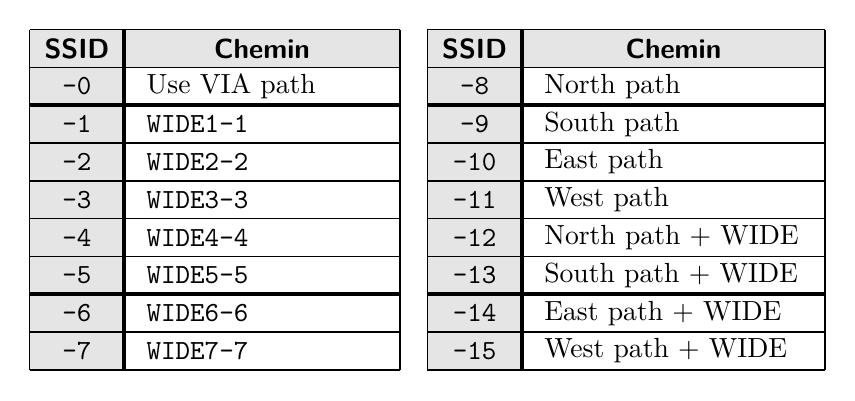
\begin{tikzpicture}[x=1cm,y=1cm,baseline=(current bounding box.north)]
  \def\rowheight{0.48}
  \def\ssidwidth{1.20}

  \begin{scope}
    \def\tablewidth{4.70}
    \fill[gray!20] (0,0) rectangle (\tablewidth,-\rowheight);
    \fill[gray!20] (0,-\rowheight) rectangle (\ssidwidth,{-9*\rowheight});
    \foreach \line in {0,...,9}
      \draw[line width=0.5pt] (0,{-\line*\rowheight}) -- (\tablewidth,{-\line*\rowheight});
    \draw[line width=1.5pt] (0,{-2*\rowheight}) -- (\tablewidth,{-2*\rowheight});
    \draw[line width=1.5pt] (0,{-7*\rowheight}) -- (\tablewidth,{-7*\rowheight});
    \draw[line width=0.5pt] (0,0) -- (0,{-9*\rowheight});
    \draw[line width=1.5pt] (\ssidwidth,0) -- (\ssidwidth,{-9*\rowheight});
    \draw[line width=0.5pt] (\tablewidth,0) -- (\tablewidth,{-9*\rowheight});

    \node[font=\sffamily\bfseries] at ({\ssidwidth/2},{-0.5*\rowheight}) {SSID};
    \node[font=\sffamily\bfseries] at ({(\ssidwidth+\tablewidth)/2},{-0.5*\rowheight}) {Chemin};
    \foreach \ssid [count=\row from 1] in {0,1,2,3,4,5,6,7}
      \node[font=\ttfamily] at ({\ssidwidth/2},{-(\row+0.5)*\rowheight}) {-\ssid};
    \node[anchor=west] at ({\ssidwidth+0.16},{-1.5*\rowheight}) {Use VIA path};
    \foreach \wide [count=\row from 2] in {1,2,3,4,5,6,7}
      \node[anchor=west,font=\ttfamily] at ({\ssidwidth+0.16},{-(\row+0.5)*\rowheight}) {WIDE\wide-\wide};
  \end{scope}

  \begin{scope}[xshift=5.05cm]
    \def\tablewidth{5.05}
    \fill[gray!20] (0,0) rectangle (\tablewidth,-\rowheight);
    \fill[gray!20] (0,-\rowheight) rectangle (\ssidwidth,{-9*\rowheight});
    \foreach \line in {0,...,9}
      \draw[line width=0.5pt] (0,{-\line*\rowheight}) -- (\tablewidth,{-\line*\rowheight});
    \draw[line width=1.5pt] (0,{-2*\rowheight}) -- (\tablewidth,{-2*\rowheight});
    \draw[line width=1.5pt] (0,{-7*\rowheight}) -- (\tablewidth,{-7*\rowheight});
    \draw[line width=0.5pt] (0,0) -- (0,{-9*\rowheight});
    \draw[line width=1.5pt] (\ssidwidth,0) -- (\ssidwidth,{-9*\rowheight});
    \draw[line width=0.5pt] (\tablewidth,0) -- (\tablewidth,{-9*\rowheight});

    \node[font=\sffamily\bfseries] at ({\ssidwidth/2},{-0.5*\rowheight}) {SSID};
    \node[font=\sffamily\bfseries] at ({(\ssidwidth+\tablewidth)/2},{-0.5*\rowheight}) {Chemin};
    \foreach \ssid [count=\row from 1] in {8,9,10,11,12,13,14,15}
      \node[font=\ttfamily] at ({\ssidwidth/2},{-(\row+0.5)*\rowheight}) {-\ssid};
    \node[anchor=west] at ({\ssidwidth+0.16},{-1.5*\rowheight}) {North path};
    \node[anchor=west] at ({\ssidwidth+0.16},{-2.5*\rowheight}) {South path};
    \node[anchor=west] at ({\ssidwidth+0.16},{-3.5*\rowheight}) {East path};
    \node[anchor=west] at ({\ssidwidth+0.16},{-4.5*\rowheight}) {West path};
    \node[anchor=west] at ({\ssidwidth+0.16},{-5.5*\rowheight}) {North path + WIDE};
    \node[anchor=west] at ({\ssidwidth+0.16},{-6.5*\rowheight}) {South path + WIDE};
    \node[anchor=west] at ({\ssidwidth+0.16},{-7.5*\rowheight}) {East path + WIDE};
    \node[anchor=west] at ({\ssidwidth+0.16},{-8.5*\rowheight}) {West path + WIDE};
  \end{scope}
\end{tikzpicture}
\end{flushleft}
\end{aprssideblock}

\begin{aprssideblock}{SSID de Source\\Address\\pour spécifier\\les symboles}
\phantomsection\addcontentsline{toc}{section}{SSID de Source Address pour spécifier les symboles}\label{ssid-de-source-address-pour-spuxe9cifier-des-symboles}
Le champ Source Address AX.25 contient l'indicatif et le SSID de la station
d'origine. Si le SSID est \texttt{-0}, APRS ne le traite d'aucune manière
particulière.

Si, en revanche, le SSID de Source Address est non nul, APRS l'interprète
comme une icône d'affichage. Cette utilisation est exclusivement destinée aux
trackers autonomes pour lesquels il n'existe aucune autre méthode permettant
de spécifier un symbole d'affichage ou une adresse de destination, par exemple
les trackers MIM ou NMEA.

Pour plus d'informations, voir le chapitre 20 : Symboles APRS.
\end{aprssideblock}

\chapter[DONNÉES APRS DANS LE CHAMP INFORMATION AX.25]{Données APRS dans le champ Information
AX.25}\label{donnuxe9es-aprs-dans-le-champ-information-ax.25}

\begin{aprssideblock}{Format générique\\des données}
\phantomsection\addcontentsline{toc}{section}{Format générique des données}\label{format-guxe9nuxe9rique-des-donnuxe9es}
En général, le champ Information AX.25 peut contenir tout ou partie des
informations suivantes :

\begin{itemize}
\tightlist
\item
  APRS Data Type Identifier
\item
  APRS Data
\item
  APRS Data Extension
\item
  Comment
\end{itemize}
\end{aprssideblock}

\begin{aprsbodyblock}
\setlength{\arrayrulewidth}{0.75pt}
\begin{tabular}{|c|c|c|c|}
\hline
\multicolumn{4}{|>{\columncolor{gray!20}}l|}{\bfseries\itshape Generic APRS Information Field}\\
\hline
\bfseries\itshape Data Type ID & \bfseries\itshape APRS Data & \bfseries\itshape APRS Data Extension & \bfseries\itshape Comment \\
\hline
\makebox[0pt][r]{Octets :\hspace{3.2em}}1 & n & 7 & n \\
\hline
\end{tabular}
\end{aprsbodyblock}

\begin{aprssideblock}{APRS Data Type\\Identifier}
\phantomsection\addcontentsline{toc}{section}{APRS Data Type Identifier}\label{aprs-data-type-identifier}
Chaque paquet APRS contient un APRS Data Type Identifier (DTI). Celui-ci
détermine le format du reste des données du champ Information, comme suit :
\end{aprssideblock}

\vspace{8pt}
\noindent\textbf{APRS Data Type Identifiers}\par\vspace{4pt}
{\footnotesize
\setlength{\tabcolsep}{4pt}
\setlength{\arrayrulewidth}{0.75pt}
\renewcommand{\arraystretch}{1.15}
\noindent
\begin{tabular}[t]{|>{\columncolor{gray!20}\centering\arraybackslash}p{26pt}|p{\dimexpr0.49\textwidth-46pt\relax}|}
\hline
\rowcolor{gray!20}
\bfseries\itshape Ident & \multicolumn{1}{>{\columncolor{gray!20}}c|}{\bfseries\itshape Data Type} \\
\hline
\texttt{0x1c} & Current Mic-E Data (Rev 0 beta) \\
\hline
\texttt{0x1d} & Old Mic-E Data (Rev 0 beta) \\
\hline
! & Position sans timestamp (sans messagerie), ou Ultimeter 2000 WX Station \\
\hline
" & \emph{[Unused]} \\
\hline
\# & Peet Bros U-II Weather Station \\
\hline
\$ & Raw GPS data ou Ultimeter 2000 \\
\hline
\% & Agrelo DFJr / MicroFinder \\
\hline
\& & \emph{[Reserved --- Map Feature]} \\
\hline
\textquotesingle{} & Old Mic-E Data (mais \emph{Current} data pour TM-D700) \\
\hline
( & \emph{[Unused]} \\
\hline
) & Item \\
\hline
* & Peet Bros U-II Weather Station \\
\hline
+ & \emph{[Reserved --- Shelter data with time]} \\
\hline
, & Invalid data ou test data \\
\hline
- & \emph{[Unused]} \\
\hline
. & \emph{[Reserved --- Space weather]} \\
\hline
/ & Position avec timestamp (sans messagerie) \\
\hline
\texttt{0–9} & \emph{[Do not use]} \\
\hline
: & Message \\
\hline
; & Object \\
\hline
\end{tabular}
\hfill
\begin{tabular}[t]{|>{\columncolor{gray!20}\centering\arraybackslash}p{26pt}|p{\dimexpr0.49\textwidth-46pt\relax}|}
\hline
\rowcolor{gray!20}
\bfseries\itshape Ident & \multicolumn{1}{>{\columncolor{gray!20}}c|}{\bfseries\itshape Data Type} \\
\hline
\textless{} & Station Capabilities \\
\hline
= & Position sans timestamp (avec messagerie APRS) \\
\hline
\textgreater{} & Status \\
\hline
? & Query \\
\hline
@ & Position avec timestamp (avec messagerie APRS) \\
\hline
\texttt{A–S} & \emph{[Do not use]} \\
\hline
T & Telemetry data \\
\hline
\texttt{U–Z} & \emph{[Do not use]} \\
\hline
{[} & Maidenhead grid locator beacon (obsolète) \\
\hline
\textbackslash{} & \emph{[Unused]} \\
\hline
{]} & \emph{[Unused]} \\
\hline
\textasciicircum{} & \emph{[Unused]} \\
\hline
\_ & Weather Report (sans position) \\
\hline
\textasciigrave{} & Current Mic-E Data (\emph{non utilisé} sur TM-D700) \\
\hline
\texttt{a–z} & \emph{[Do not use]} \\
\hline
\{ & User-Defined APRS packet format \\
\hline
\textbar{} & \emph{[Do not use --- TNC stream switch character]} \\
\hline
\} & Third-party traffic \\
\hline
\textasciitilde{} & \emph{[Do not use --- TNC stream switch character]} \\
\hline
\end{tabular}
}

\begin{aprsbodyblock}
Note : la radio Kenwood TM-D700 utilise le DTI \lit{\textquotesingle{}} pour
les données Mic-E actuelles (\emph{current}). Cette radio n'utilise pas le
DTI \lit{\textasciigrave{}}.
\end{aprsbodyblock}

\begin{aprssideblock}{APRS Data and\\Data Extension}
\phantomsection\addcontentsline{toc}{section}{APRS Data and Data Extension}\label{aprs-data-and-data-extension}
Il existe 10 types principaux d'APRS Data :

\begin{itemize}
\tightlist
\item
  Position
\item
  Direction Finding
\item
  Objects and Items
\item
  Weather
\item
  Telemetry
\item
  Messages, Bulletins and Announcements
\item
  Queries
\item
  Responses
\item
  Status
\item
  Other
\end{itemize}

Certaines de ces données peuvent également comporter une APRS Data
Extension, qui fournit des informations supplémentaires.

L'APRS Data et l'APRS Data Extension optionnelle suivent le Data Type
Identifier.

Le tableau de la page suivante présente une liste complète de tous les
différents types possibles d'APRS Data et d'APRS Data Extension.
\end{aprssideblock}

\begin{center}
{\footnotesize
\setlength{\tabcolsep}{4pt}
\setlength{\arrayrulewidth}{0.75pt}
\begin{tabular}{|>{\columncolor{gray!20}\raggedleft\arraybackslash\bfseries}m{0.15\linewidth}|>{\raggedright\arraybackslash}p{0.38\linewidth}|>{\raggedright\arraybackslash}p{0.38\linewidth}|}
\hline
\rowcolor{gray!20}
 & \multicolumn{1}{c|}{\bfseries\itshape Possible APRS Data} & \multicolumn{1}{c|}{\bfseries\itshape Possible APRS Data Extension} \\
\hline

Position &
Time (DHM or HMS)\newline
Lat/long coordinates\newline
Compressed lat/long/course/speed/radio range/altitude\newline
Symbol Table ID and Symbol Code\newline
Mic-E longitude, speed and course, telemetry or status\newline
Raw GPS NMEA sentence\newline
Raw weather station data &
Course and Speed\newline
Power, Effective Antenna Height/Gain/Directivity\newline
Pre-Calculated Radio Range\newline
Omni DF Signal Strength\newline
Storm Data (in Comment field) \\
\hline
Direction Finding &
Time (DHM or HMS)\newline
Lat/long coordinates\newline
Compressed lat/long/course/speed/radio range/altitude\newline
Symbol Table ID and Symbol Code &
Course and Speed\newline
Power, Effective Antenna Height/Gain/Directivity\newline
Pre-Calculated Radio Range\newline
Omni DF Signal Strength\newline
Bearing and Number/Range/Quality (in Comment field) \\
\hline
Objects and Items &
Object name\newline
Item name\newline
Time (DHM or HMS)\newline
Lat/long coordinates\newline
Compressed lat/long/course/speed/radio range/altitude\newline
Symbol Table ID and Symbol Code\newline
Raw weather station data &
Course and Speed\newline
Power, Effective Antenna Height/Gain/Directivity\newline
Pre-Calculated Radio Range\newline
Omni DF Signal Strength\newline
Area Object\newline
Storm Data (in Comment field) \\
\hline
Weather &
Time (MDHM)\newline
Lat/long coordinates\newline
Compressed lat/long/course/speed/radio range/altitude\newline
Symbol Table ID and Symbol Code\newline
Raw weather station data &
Wind Direction and Speed\newline
Storm Data (in Comment field) \\
\hline
Telemetry &
Telemetry (non Mic-E) & \\
\hline
Messages, Bulletins and Announcements &
Addressee\newline
Message Text\newline
Message Identifier\newline
Message Acknowledgement\newline
Bulletin ID, Announcement ID\newline
Group Bulletin ID & \\
\hline
Queries &
Query Type\newline
Query Target Footprint\newline
Addressee (Directed Query) & \\
\hline
Responses &
Position\newline
Object/Item\newline
Weather\newline
Status\newline
Message\newline
Digipeater Trace\newline
Stations Heard\newline
Heard Statistics\newline
Station Capabilities &
Course and Speed\newline
Power, Effective Antenna Height/Gain/Directivity\newline
Pre-Calculated Radio Range\newline
Omni DF Signal Strength\newline
Area Object\newline
Wind Direction and Speed \\
\hline
Status &
Time (DHM zulu)\newline
Status text\newline
Meteor Scatter Beam Heading/Power\newline
Maidenhead Locator (Grid Square)\newline
Altitude (Mic-E)\newline
E-mail message & \\
\hline
Other &
Third-Party forwarding\newline
Invalid Data/Test Data & \\
\hline
\end{tabular}
}
\end{center}

\begin{aprssideblock}{Comment Field}
\phantomsection\addcontentsline{toc}{section}{Comment Field}\label{comment-field}
En général, tout paquet APRS peut contenir un commentaire en texte libre
(tel qu'un message de beacon) dans le champ Information, immédiatement après
les APRS Data ou l'APRS Data Extension.

Il n'y a pas de séparateur entre les données APRS et le commentaire, sauf
mention contraire.

Le commentaire peut contenir tout caractère ASCII imprimable ou UTF-8 (à
l'exception de \lit{\textbar{}} et \lit{\textasciitilde{}}, réservés au TNC
channel switching).

Ne placez aucun retour chariot (0x0d) ni saut de ligne (0x0a) à la fin. Les
stations IGate les supprimeront, ce qui produira un contenu légèrement
différent.

La longueur maximale, très faible et apparemment arbitraire, du champ
Comment dépend du rapport concerné --- les détails figurent dans la
description de chaque rapport.

Dans certains cas particuliers, le champ Comment peut également contenir des
données APRS supplémentaires :

\begin{itemize}
\tightlist
\item
  \textbf{Altitude} dans le texte de commentaire (voir chapitre 6 : Formats
  de temps et de position), ou dans le texte de statut Mic-E (voir chapitre
  10 : Format Mic-E).
\item
  \textbf{Maidenhead Locator} (grid square), dans un champ de texte de
  statut Mic-E (voir chapitre 10 : Format Mic-E) ou dans un Status Report
  (voir chapitre 16 : Rapports de statut).
\item
  Les paramètres \textbf{Bearing and Number/Range/Quality}
  (\texttt{/BRG/NRQ}), dans les DF reports (voir chapitre 7 : Extensions de
  données APRS).
\item
  \textbf{Area Object Line Widths} (voir chapitre 11 : Rapports d'Objets et
  d'Items).
\item
  \textbf{Signpost Objects} (voir chapitre 11 : Rapports d'Objets et
  d'Items).
\item
  \textbf{Weather and Storm Data} (voir chapitre 12 : Rapports météo).
\item
  \textbf{Beam Heading and Power}, dans les Status Reports (voir chapitre
  16 : Rapports de statut).
\end{itemize}
\end{aprssideblock}

\begin{aprssideblock}{Base-91\\Notation}
\phantomsection\addcontentsline{toc}{section}{Base-91 Notation}\label{notation-base-91}
Deux formats de données APRS utilisent la notation base-91 : les
coordonnées lat/long au format compressé (voir chapitre 9 : Formats
compressés de rapport de position) et l'altitude au format Mic-E (voir
chapitre 10 : Format Mic-E).

Les données base-91 sont compressées en une courte chaîne de caractères.
Tous les caractères sont des caractères ASCII imprimables, avec des codes de
caractère compris entre 33 et 124 en décimal (c'est-à-dire de \lit{!} à
\lit{\textbar{}}).

Pour calculer la chaîne de caractères ASCII base-91 correspondant à une
valeur de donnée donnée, cette valeur est divisée par des puissances de 91
progressivement décroissantes jusqu'à ce que le reste soit inférieur à 91. À
chaque étape, 33 est ajouté au modulo de la division pour obtenir le code de
caractère ASCII correspondant.

Par exemple, pour une valeur de donnée de 12345678 :

\begin{verbatim}
12345678 / 91³ = modulo 16, reste 288542
288542   / 91² = modulo 34, reste 6988
6988     / 91¹ = modulo 76, reste 72
\end{verbatim}

Les quatre codes de caractère ASCII sont donc 49 (c'est-à-dire 16+33), 67
(c'est-à-dire 34+33), 109 (c'est-à-dire 76+33) et 105 (c'est-à-dire 72+33),
correspondant à la chaîne ASCII \texttt{1Cmi}.
\end{aprssideblock}

\begin{aprssideblock}{APRS Precision\\and Datum Option}
\phantomsection\addcontentsline{toc}{section}{APRS Precision and Datum Option}\label{aprs-precision-and-datum-option}
Cette extension de la spécification APRS permet de transmettre une plus
grande précision entre utilisateurs. Mais comme la précision sans
l'exactitude du datum n'a pas de sens, ce format inclut également
l'identification du datum utilisé pour obtenir cette précision.

\textbf{DATUM :} le datum par défaut pour le GPS et pour APRS est WGS84. La
spécification APRS indique que toutes les positions on-air sont présumées
être en WGS84 sauf indication contraire. Cette \guillemotleft{}option\guillemotright{}
documente donc deux méthodes pour \guillemotleft{}indiquer autrement\guillemotright{} :

\textbf{PAR PAYS :} ou par accord local continental. Deux accords de ce type
ont été déclarés : WGS84 en Amérique du Nord et OSGB36 au Royaume-Uni. Si
d'autres peuvent être convenus, ils seront listés.

\textbf{PAR DATUM BYTE :} le DATUM byte dans cette \guillemotleft{}PRECISION
and DATUM Option\guillemotright{}.

\textbf{FORMAT :} le format de cette option APRS Precision-and-Datum est la
présence d'un champ de 5 octets \texttt{!DAO!} apparaissant n'importe où dans
le champ de commentaire de position. Cette option est rétrocompatible car le
format de base DDMM.mmN/DDDMM.mmH est conservé et sera toujours décodé par
toutes les applications existantes. Le \texttt{!DAO!} fournit simplement la
précision supplémentaire jusqu'à environ un pied (30~cm) et identifie
également le datum :

\begin{verbatim}
!DAO! - longueur fixe, n'importe où dans le commentaire de position
 D    - identifiant du datum (base-91)
  A   - précision supplémentaire de LAtitude (base-91)
   O  - précision supplémentaire de LOngitude (base-91)
\end{verbatim}

\textbf{RECOMMANDATION :} il est recommandé de placer cette option à la FIN
de tout autre texte de commentaire de position. Ainsi, elle ne déplace aucun
texte de commentaire lisible par un humain que l'on souhaiterait afficher sur
les anciens systèmes. Cette option ajoutée peut dépasser la limite
\guillemotleft{}visible\guillemotright{} actuelle de 57 octets de la
spécification, puisque ces octets supplémentaires ne sont de toute façon pas
utilisés par les systèmes existants.

\textbf{PRÉCISION :} cette option offre trois degrés de précision.

\begin{enumerate}
\item \textbf{LISIBLE HUMAINEMENT, millièmes de minute.} Précis à environ
  6 pieds (2~m) près et, étant lisible humainement, permet même aux
  utilisateurs de D7, D700 ou de toute autre application existante de lire
  une position à 3 décimales de minutes. Ce format est identifié si le Datum
  byte est en majuscule.

\item \textbf{BASE-91.} Ajoute une précision supplémentaire au
  91/10\,000\textsuperscript{e} de minute près, soit environ 4 chiffres
  fractionnaires décimaux de minute, soit environ un pied (30~cm). Ce format
  est identifié si le datum byte est en minuscule.

\item \textbf{NULL.} Si les octets A et O sont des caractères ESPACE, ils ne
  sont présents que pour respecter le format \texttt{!DAO!} et n'impliquent
  AUCUNE précision ajoutée. Utilisé lorsqu'on souhaite envoyer une
  information de DATUM sans revendiquer de précision supplémentaire. Cette
  utilisation de caractères espace pour indiquer l'absence de chiffres de
  précision est cohérente avec le système d'ambiguïté APRS existant.
\end{enumerate}

\textbf{DATUMS :} plusieurs catégories de datums peuvent être utilisées.

\textbf{PRÉDÉFINIS :} les lettres A--Z et a--z indiquent l'un des 26 datums
courants. La casse de ces 26 lettres indique le type de précision utilisé.
Les majuscules indiquent des chiffres décimaux lisibles pour A et O, et les
minuscules indiquent un encodage base-91 pour A et O. Il existe 26 DATUMS
prédéfinis. Une table des 26 datums courants sera préparée. Voici quelques
exemples :

\begin{verbatim}
W = WGS84
N = NAD27
O = OSGB36
\end{verbatim}

\textbf{LOCAL CUSTOM :} pour des événements spéciaux et fermés, le DATUM
peut être l'une des dix options définies localement. Elles sont indiquées par
les chiffres 0 à 9. Une utilisation créative consiste, pour des événements
fermés utilisant des cartes ou des lieux fixes, à définir les cartes par
numéro~!

\textbf{ENCODAGE BASE-91 :} le base-91 est fréquemment utilisé en APRS pour
améliorer la résolution d'un octet sans utiliser de binaire et en
n'utilisant que le sous-ensemble de caractères ASCII imprimables. L'usage
exclusif de caractères ASCII imprimables présente de nombreux avantages qui
ont été abondamment discutés par ailleurs. Le base-91 signifie simplement la
valeur d'un octet ASCII après soustraction de 33 en décimal. Ainsi le
caractère \guillemotleft{}\texttt{!}\guillemotright{} moins 33 donne
\guillemotleft{}0\guillemotright{}, jusqu'au caractère
\guillemotleft{}\texttt{\}}\guillemotright{} moins 33 qui donne la valeur
\guillemotleft{}90\guillemotright{}.

\textbf{AUTRES :} il reste 28 autres possibilités d'information de DATUM
dans le chiffre D qui peuvent être utilisées si nécessaire.

\textbf{Exemples :}

\texttt{!W23!} signifie WGS84 et la majuscule indique qu'il s'agit du
format lisible humainement au 3\textsuperscript{e} chiffre. \guillemotleft{}2\guillemotright{}
est le troisième chiffre décimal des minutes de latitude et est lisible
humainement. \guillemotleft{}3\guillemotright{} est le chiffre ajouté des
minutes de longitude et est également lisible humainement.

\texttt{!wAb!} signifie WGS84 mais la minuscule indique qu'il s'agit de la
précision ajoutée au pied près. \guillemotleft{}A\guillemotright{} est le
code base-91 pour deux chiffres supplémentaires (65 moins 33 donne
\guillemotleft{}32\guillemotright{}) et \guillemotleft{}b\guillemotright{}
donne deux chiffres supplémentaires de longitude (98 -- 33, soit
\guillemotleft{}...65\guillemotright{}).

\texttt{!w:\textbackslash!} serait également WGS84 mais avec
\guillemotleft{}:\guillemotright{} et \guillemotleft{}\textbackslash\guillemotright{}
décodant deux chiffres supplémentaires de \guillemotleft{}27\guillemotright{}
pour la latitude et \guillemotleft{}59\guillemotright{} pour la longitude,
au pied près environ.

\textbf{CONVERSION BASE-91 :} dans le premier exemple \texttt{!W23!}
ci-dessus, les chiffres réels sont simplement ajoutés aux LAT/LONG
existantes, par exemple pour ajouter de la précision à DDMM.mmN/DDDMM.mmH
et devenir équivalent à DDMM.mm2N et DDDMM.mm3H.

Mais dans les deux exemples suivants \texttt{!wAb!} et \texttt{!w:\textbackslash!},
les deux chiffres ajoutés ne peuvent pas être simplement ajoutés à la chaîne
de position ASCII, puisqu'ils ne peuvent aller que de 00 à 90. Il faut donc
les mettre à l'échelle pour qu'ils aillent de 00 à 99. Pour ce faire,
multiplier les deux chiffres par 1,10. Ainsi, pour l'exemple
\texttt{!wAb!} avec des chiffres de latitude ajoutés de 32, on multiplie
par 1,10 pour obtenir des chiffres réels ajoutés de 35,2. La position en
haute précision devient alors DDMM.mm352N.
\end{aprssideblock}

\begin{aprssideblock}{APRS Data\\Units}
\phantomsection\addcontentsline{toc}{section}{APRS Data Units}\label{unituxe9s-de-donnuxe9es-aprs}
Pour des raisons historiques, il existe un certain manque de cohérence entre
les unités de données dans les paquets APRS --- certaines vitesses sont
exprimées en knots (nœuds), d'autres en miles per hour (miles par heure) ;
certaines altitudes sont exprimées en pieds, d'autres en mètres, et ainsi de
suite. Il est souligné que cette spécification décrit les unités de données
telles qu'elles sont transmises sur l'air (\emph{on-air}). Il incombe aux
applications APRS de convertir les unités on-air en unités plus appropriées
si nécessaire.

Le datum terrestre GPS par défaut est le World Geodetic System (WGS) 1984,
mais des options continentales telles que OSG pour le Royaume-Uni sont
acceptables.
\end{aprssideblock}

\chapter[FORMATS DE TEMPS ET DE POSITION]{Formats de temps et de
position}\label{formats-de-temps-et-de-position}

\section{Formats de temps}\label{formats-de-temps}

Les timestamps APRS s'expriment de 3 manières :

\begin{itemize}
\tightlist
\item
  Day/Hours/Minutes (DHM)
\item
  Hours/Minutes/Seconds (HMS)
\item
  Month/Day/Hours/Minutes (MDHM)
\end{itemize}

Toutes utilisent l'horloge 24 h.

\textbf{DHM} --- champ fixe de 7 caractères : 6 chiffres (jour + heure)
+ 1 indicateur (\texttt{z} ou \texttt{/}). Le groupe est
\texttt{JJHHMM}, jour du mois 01-31, heures et minutes.

\begin{itemize}
\tightlist
\item
  \texttt{092345z} = 23:45 zulu, jour 9 du mois.
\item
  \texttt{092345/} = 23:45 heure locale, jour 9.
\end{itemize}

Recommandé : n'émettre que du zulu à l'avenir. Les Status Reports
n'acceptent que le zulu.

\textbf{HMS} --- champ fixe de 7 caractères : 6 chiffres
(heures/minutes/secondes) + \texttt{h}.

\begin{itemize}
\tightlist
\item
  \texttt{234517h} = 23:45:17 zulu.
\end{itemize}

Non utilisable dans les Status Reports.

\textbf{MDHM} --- champ fixe de 8 caractères : mois (01-12), jour
(01-31), heures + minutes zulu.

\begin{itemize}
\tightlist
\item
  \texttt{10092345} = 23:45 zulu le 9 octobre.
\end{itemize}

Utilisé uniquement dans les rapports de stations météo « positionless ».

\section{Usage des timestamps}\label{usage-des-timestamps}

Quand une station émet un rapport sans timestamp, une station APRS
réceptrice peut noter en interne l'heure de réception. C'est la vision «
émission = maintenant » côté récepteur.

Quand une station émet un rapport avec timestamp, ce timestamp
représente l'heure de création côté émetteur.

Autrement dit : - rapport sans timestamp = temps réel, courant (le
récepteur note l'heure). - rapport avec timestamp = pas nécessairement
temps réel, potentiellement (très) ancien.

Quatre DTIs indiquent si le rapport contient ou non un timestamp, selon
que la station a la capacité messagerie APRS ou non :

\begin{longtable}[]{@{}lll@{}}
\toprule\noalign{}
& Sans messagerie APRS & Avec messagerie APRS \\
\midrule\noalign{}
\endhead
\bottomrule\noalign{}
\endlastfoot
Sans timestamp (courant) & \texttt{!} & \texttt{=} \\
Avec timestamp (ancien / différé) & \texttt{/} & \texttt{@} \\
\end{longtable}

Stations sans messagerie = généralement trackers autonomes ou
digipeaters. Stations sans timestamp = généralement stations fixes.

\section{Format latitude}\label{format-latitude}

Champ fixe 8 caractères : degrés + minutes décimales (2 décimales) +
\texttt{N} ou \texttt{S}.

\begin{itemize}
\tightlist
\item
  Degrés : 00 à 90.
\item
  Minutes : entier + centièmes, séparés par un point.
\end{itemize}

Ex : \texttt{4903.50N} = 49° 3' 30'' nord.

Notation générique : chaîne \texttt{ddmm.hhN}.

\section{Format longitude}\label{format-longitude}

Champ fixe 9 caractères : degrés + minutes décimales (2 décimales) +
\texttt{E} ou \texttt{W}.

\begin{itemize}
\tightlist
\item
  Degrés : 000 à 180.
\item
  Minutes : entier + centièmes.
\end{itemize}

Ex : \texttt{07201.75W} = 72° 1' 45'' ouest.

Notation générique : \texttt{dddmm.hhW}.

\section{Coordonnées de position}\label{coordonnuxe9es-de-position}

Combinaison lat + long séparées par un Symbol Table Identifier, suivies
d'un Symbol Code.

Ex : \texttt{4903.50N/07201.75W-} --- \texttt{/} = table de symboles
primaire, \texttt{-} = icône « maison ».

Voir chapitre 20 et annexe 2 pour les symboles.

\section{Ambiguïté de position}\label{ambiguuxeftuxe9-de-position}

Quand la position exacte n'est pas connue, on peut réduire la précision
en remplaçant progressivement \texttt{mm} puis \texttt{hh} de la
latitude par des espaces (\texttt{V}) :

\begin{itemize}
\tightlist
\item
  \texttt{4903.5VN} = latitude au dixième de minute.
\item
  \texttt{4903.VVN} = à la minute.
\item
  \texttt{490V.VVN} = à 10 minutes.
\item
  \texttt{49VV.VVN} = au degré.
\end{itemize}

Le niveau d'ambiguïté de la latitude s'applique automatiquement à la
longitude --- inutile d'y ajouter des \texttt{V}.

Ex : \texttt{4903.VVN/07201.75W-} = position au plus proche de la
minute. Les centièmes de minutes en lat/long peuvent prendre n'importe
quelle valeur 00-99. Bounding box : - NW : 49° 3.99' N, 72° 1.99' W - NE
: 49° 3.99' N, 72° 1.00' W - SE : 49° 3.00' N, 72° 1.00' W - SW : 49°
3.00' N, 72° 1.99' W

\section{Position nulle par
défaut}\label{position-nulle-par-duxe9faut}

Quand une station n'a pas de position spécifique (ex : Mic-E sans GPS
connecté), elle doit émettre une position nulle par défaut : 0° 0' 0''
N, 0° 0' 0'' W, avec le symbole \texttt{\textbackslash{}.} (position
inconnue).

Ex : \texttt{…0000.00N\textbackslash{}00000.00W.…}

\section{Locator Maidenhead (Grid
Square)}\label{locator-maidenhead-grid-square}

Alternative à la lat/long. Quatre manières :

\begin{itemize}
\tightlist
\item
  Dans un Status Report : \texttt{IO91SX/(} (\texttt{/-} = symbole
  maison).
\item
  Dans le Mic-E Status Text : \texttt{IO91SX/G} (\texttt{/G} = « grid
  square »).
\item
  Dans le champ Destination (obsolète) : \texttt{IO91SX}.
\item
  Dans un beacon AX.25 avec DTI \texttt{{[}} (obsolète) :
  \texttt{{[}IO91SX{]}}.
\end{itemize}

Le grid square est en forme 6 caractères ou raccourcie 4 caractères
(\texttt{IO91}).

\section{Données NMEA}\label{donnuxe9es-nmea}

APRS reconnaît les chaînes ASCII brutes conformes NMEA 0183 v2.0
provenant de GPS ou LORAN. Recommandé d'interpréter au moins :

\begin{longtable}[]{@{}ll@{}}
\toprule\noalign{}
Sentence & Signification \\
\midrule\noalign{}
\endhead
\bottomrule\noalign{}
\endlastfoot
\texttt{GGA} & Global Positioning System Fix Data \\
\texttt{GLL} & Geographic Position, Latitude/Longitude Data \\
\texttt{RMC} & Recommended Minimum Specific GPS/Transit Data \\
\texttt{VTG} & Velocity and Track Data \\
\texttt{WPT} & Way Point Location \\
\end{longtable}

\section{Altitude}\label{altitude}

Deux façons :

\begin{itemize}
\tightlist
\item
  \textbf{Dans le comment text} --- format \texttt{/A=aaaaaa},
  \texttt{aaaaaa} = altitude en \textbf{pieds}. Ex : \texttt{/A=001234}.
  Peut apparaître n'importe où dans le commentaire.
\item
  \textbf{En format Mic-E} --- champ statut Mic-E optionnel. Voir
  chapitre 10.
\end{itemize}

\begin{center}\rule{0.5\linewidth}{0.5pt}\end{center}

\chapter[EXTENSIONS DE DONNÉES APRS]{Extensions de données
APRS}\label{extensions-de-donnuxe9es-aprs}

Un champ fixe de 7 octets peut suivre les données de position APRS.
Types d'extension :

\begin{itemize}
\tightlist
\item
  \texttt{CSE/SPD} --- Course and Speed (peut être suivi de 8 octets
  supplémentaires : bearing DF + NRQ).
\item
  \texttt{DIR/SPD} --- Wind Direction and Wind Speed.
\item
  \texttt{PHGphgd} --- Power + Height/Gain/Directivity.
\item
  \texttt{RNGrrrr} --- Pre-Calculated Radio Range.
\item
  \texttt{DFSshgd} --- DF Signal Strength + Height/Gain.
\item
  \texttt{Tyy/Cxx} --- Area Object Descriptor.
\end{itemize}

\section*{Course and Speed}\label{course-and-speed}

Course en degrés 001-360 (nord = 360, sens horaire). Vitesse en knots.
Séparateur \texttt{/}.

Ex : \texttt{088/036} = cap 88°, 36 knots.

Si inconnu : \texttt{000/000}, \texttt{.../...} ou \texttt{VVV/VVV}.

\textbf{Cas DF} : \texttt{000} = station DF fixe ; non nul = mobile.

\section*{Wind Direction and Wind
Speed}\label{wind-direction-and-wind-speed}

Direction du vent en degrés 001-360. Vitesse en knots. Séparateur
\texttt{/}. Vitesse soutenue sur 1 minute.

Ex : \texttt{220/004} = vent de 220° à 4 knots.

\section*{Power, Effective Antenna
Height/Gain/Directivity}\label{power-effective-antenna-heightgaindirectivity}

Format \texttt{PHGphgd} --- 7 caractères. Sert à tracer un cercle de
portée radio autour de la station.

\begin{itemize}
\tightlist
\item
  Caractères 1-3 : \texttt{PHG} fixe.
\item
  Char 4 : \texttt{p} code puissance.
\item
  Char 5 : \texttt{h} code hauteur.
\item
  Char 6 : \texttt{g} code gain antenne.
\item
  Char 7 : \texttt{d} code directivité.
\end{itemize}

Codes PHG :

\begin{longtable}[]{@{}
  >{\raggedright\arraybackslash}p{(\columnwidth - 22\tabcolsep) * \real{0.0833}}
  >{\raggedright\arraybackslash}p{(\columnwidth - 22\tabcolsep) * \real{0.0833}}
  >{\raggedright\arraybackslash}p{(\columnwidth - 22\tabcolsep) * \real{0.0833}}
  >{\raggedright\arraybackslash}p{(\columnwidth - 22\tabcolsep) * \real{0.0833}}
  >{\raggedright\arraybackslash}p{(\columnwidth - 22\tabcolsep) * \real{0.0833}}
  >{\raggedright\arraybackslash}p{(\columnwidth - 22\tabcolsep) * \real{0.0833}}
  >{\raggedright\arraybackslash}p{(\columnwidth - 22\tabcolsep) * \real{0.0833}}
  >{\raggedright\arraybackslash}p{(\columnwidth - 22\tabcolsep) * \real{0.0833}}
  >{\raggedright\arraybackslash}p{(\columnwidth - 22\tabcolsep) * \real{0.0833}}
  >{\raggedright\arraybackslash}p{(\columnwidth - 22\tabcolsep) * \real{0.0833}}
  >{\raggedright\arraybackslash}p{(\columnwidth - 22\tabcolsep) * \real{0.0833}}
  >{\raggedright\arraybackslash}p{(\columnwidth - 22\tabcolsep) * \real{0.0833}}@{}}
\toprule\noalign{}
\begin{minipage}[b]{\linewidth}\raggedright
Code
\end{minipage} & \begin{minipage}[b]{\linewidth}\raggedright
0
\end{minipage} & \begin{minipage}[b]{\linewidth}\raggedright
1
\end{minipage} & \begin{minipage}[b]{\linewidth}\raggedright
2
\end{minipage} & \begin{minipage}[b]{\linewidth}\raggedright
3
\end{minipage} & \begin{minipage}[b]{\linewidth}\raggedright
4
\end{minipage} & \begin{minipage}[b]{\linewidth}\raggedright
5
\end{minipage} & \begin{minipage}[b]{\linewidth}\raggedright
6
\end{minipage} & \begin{minipage}[b]{\linewidth}\raggedright
7
\end{minipage} & \begin{minipage}[b]{\linewidth}\raggedright
8
\end{minipage} & \begin{minipage}[b]{\linewidth}\raggedright
9
\end{minipage} & \begin{minipage}[b]{\linewidth}\raggedright
Unités
\end{minipage} \\
\midrule\noalign{}
\endhead
\bottomrule\noalign{}
\endlastfoot
Power & 0 & 1 & 4 & 9 & 16 & 25 & 36 & 49 & 64 & 81 & watts \\
Height & 10 & 20 & 40 & 80 & 160 & 320 & 640 & 1280 & 2560 & 5120 &
feet \\
Gain & 0 & 1 & 2 & 3 & 4 & 5 & 6 & 7 & 8 & 9 & dB \\
Directivity & omni & 45 NE & 90 E & 135 SE & 180 S & 225 SW & 270 W &
315 NW & 360 N & & deg \\
\end{longtable}

Le code Height représente la \textbf{hauteur effective au-dessus du
terrain moyen local}, pas au-dessus du sol ni du niveau de la mer. Le
code peut être n'importe quel ASCII à partir de \texttt{0} --- pour
ballons, avions, satellites : - \texttt{:} = 10240 pieds
(\textasciitilde1.9 miles). - \texttt{;} = 20480 pieds
(\textasciitilde3.9 miles), etc.

Le code Directivity décale le cercle PHG d'un tiers dans la direction
indiquée (front-to-back 2:1). Utilisé pour signaler une direction
favorisée ou un null, même sur antenne omni.

Ex : \texttt{PHG5132} = 25 W, 20 ft d'antenne au-dessus du terrain moyen
local, 3 dB de gain, gain max plein est.

\section*{Range Circle Plot}\label{range-circle-plot}

APRS calcule la portée radio utilisable (en miles) pour tracer le cercle
:

\begin{verbatim}
power = p²
haat = 10 × 2^h                            (feet)
gain = 10^(g/10)
range = √(2 × haat × √((power/10) × (gain/2)))
\end{verbatim}

Ex \texttt{PHG5132} :

\begin{verbatim}
power = 5² = 25 W
haat = 10 × 2¹ = 20 ft
gain = 10^(3/10) = 1.995262
range = √(2 × 20 × √((25/10) × (1.995262/2))) ≈ 7.9 miles
\end{verbatim}

Comme le gain max est plein est, APRS trace un cercle de rayon 8 miles,
décalé de 2.7 miles (1/3 de 8) vers l'est.

\textbf{En l'absence de données PHG}, les stations sont supposées 10 W,
3 dB omni, 20 ft → cercle 6 miles centré sur la station.

\section*{Pre-Calculated Radio
Range}\label{pre-calculated-radio-range}

Format \texttt{RNGrrrr} --- 7 octets. \texttt{rrrr} = portée en miles
avec zéros de tête.

Ex : \texttt{RNG0050} = 50 miles. APRS trace un cercle correspondant.

\section*{Omni-DF Signal Strength}\label{omni-df-signal-strength}

Format \texttt{DFSshgd} --- 7 octets. Permet à APRS de localiser un
brouilleur en traçant les contours de force de signal des stations qui
l'entendent. Remplace \texttt{PHG} : la puissance est remplacée par la
force relative \texttt{s} (0 à 9).

Codes DFS :

\begin{longtable}[]{@{}
  >{\raggedright\arraybackslash}p{(\columnwidth - 22\tabcolsep) * \real{0.0833}}
  >{\raggedright\arraybackslash}p{(\columnwidth - 22\tabcolsep) * \real{0.0833}}
  >{\raggedright\arraybackslash}p{(\columnwidth - 22\tabcolsep) * \real{0.0833}}
  >{\raggedright\arraybackslash}p{(\columnwidth - 22\tabcolsep) * \real{0.0833}}
  >{\raggedright\arraybackslash}p{(\columnwidth - 22\tabcolsep) * \real{0.0833}}
  >{\raggedright\arraybackslash}p{(\columnwidth - 22\tabcolsep) * \real{0.0833}}
  >{\raggedright\arraybackslash}p{(\columnwidth - 22\tabcolsep) * \real{0.0833}}
  >{\raggedright\arraybackslash}p{(\columnwidth - 22\tabcolsep) * \real{0.0833}}
  >{\raggedright\arraybackslash}p{(\columnwidth - 22\tabcolsep) * \real{0.0833}}
  >{\raggedright\arraybackslash}p{(\columnwidth - 22\tabcolsep) * \real{0.0833}}
  >{\raggedright\arraybackslash}p{(\columnwidth - 22\tabcolsep) * \real{0.0833}}
  >{\raggedright\arraybackslash}p{(\columnwidth - 22\tabcolsep) * \real{0.0833}}@{}}
\toprule\noalign{}
\begin{minipage}[b]{\linewidth}\raggedright
Code
\end{minipage} & \begin{minipage}[b]{\linewidth}\raggedright
0
\end{minipage} & \begin{minipage}[b]{\linewidth}\raggedright
1
\end{minipage} & \begin{minipage}[b]{\linewidth}\raggedright
2
\end{minipage} & \begin{minipage}[b]{\linewidth}\raggedright
3
\end{minipage} & \begin{minipage}[b]{\linewidth}\raggedright
4
\end{minipage} & \begin{minipage}[b]{\linewidth}\raggedright
5
\end{minipage} & \begin{minipage}[b]{\linewidth}\raggedright
6
\end{minipage} & \begin{minipage}[b]{\linewidth}\raggedright
7
\end{minipage} & \begin{minipage}[b]{\linewidth}\raggedright
8
\end{minipage} & \begin{minipage}[b]{\linewidth}\raggedright
9
\end{minipage} & \begin{minipage}[b]{\linewidth}\raggedright
Unités
\end{minipage} \\
\midrule\noalign{}
\endhead
\bottomrule\noalign{}
\endlastfoot
Strength & 0 & 1 & 2 & 3 & 4 & 5 & 6 & 7 & 8 & 9 & S-points \\
Height & 10 & 20 & 40 & 80 & 160 & 320 & 640 & 1280 & 2560 & 5120 &
feet \\
Gain & 0 & 1 & 2 & 3 & 4 & 5 & 6 & 7 & 8 & 9 & dB \\
Directivity & omni & 45 NE & 90 E & 135 SE & 180 S & 225 SW & 270 W &
315 NW & 360 N & & deg \\
\end{longtable}

Ex : \texttt{DFS2360} = signal S2 sur antenne omni 6 dB à 80 pieds.

Une force \texttt{0} est particulièrement significative : APRS s'en sert
pour tracer (souvent en noir) des cercles où le brouilleur n'est
\textbf{pas} entendu. Beaucoup de valeur : bien plus de stations
n'entendent pas le brouilleur que le contraire.

\section*{Bearing / Number / Range / Quality
(BRG/NRQ)}\label{bearing-number-range-quality-brgnrq}

Champ 8 octets \texttt{/BRG/NRQ} suivant l'extension \texttt{CSE/SPD}.
Spécifie course, vitesse, bearing et NRQ (Number/Range/Quality).

Ex : \texttt{…088/036/270/729…} --- course=88°, vitesse=36 knots,
bearing=270°, N=7, R=2, Q=9.

\begin{itemize}
\tightlist
\item
  \texttt{N=0} → NRQ non significatif.
\item
  \texttt{N=1..8} → nombre de hits par période relatif à la longueur de
  la période (8 = 100 \%).
\item
  \texttt{N=9} → rapport manuel.
\item
  N n'est pas traité, c'est juste un indicateur des unités DF
  automatiques.
\end{itemize}

Range = \texttt{2\^{}R} (miles). Ex \texttt{R=4} → 16 miles.

Q (0-9) donne la précision du bearing :

\begin{longtable}[]{@{}llll@{}}
\toprule\noalign{}
Q & Précision & Q & Précision \\
\midrule\noalign{}
\endhead
\bottomrule\noalign{}
\endlastfoot
0 & Inutile & 5 & \textless{} 16° \\
1 & \textless{} 240° & 6 & \textless{} 8° \\
2 & \textless{} 120° & 7 & \textless{} 4° \\
3 & \textless{} 64° & 8 & \textless{} 2° \\
4 & \textless{} 32° & 9 & \textless{} 1° (meilleur) \\
\end{longtable}

Si course/speed non pertinents : \texttt{000/000}, \texttt{.../...} ou
\texttt{VVV/VVV}.

\section*{Area Object Descriptor}\label{area-object-descriptor}

Format \texttt{Tyy/Cxx} --- 7 octets. \texttt{T} = type d'objet (carré,
cercle, triangle, etc.), \texttt{/C} = couleur de remplissage. Voir
chapitre 11.

\begin{center}\rule{0.5\linewidth}{0.5pt}\end{center}

\chapter[FORMATS DE RAPPORTS DE POSITION ET RADIOGONIOMÈTRIE (DF)]{Formats de rapports de position et
radiogoniomètrie (DF)}\label{formats-de-rapports-de-position-et-radiogoniomètrie (DF)}

\newfontfamily{\cheightspacesymbolfont}{FreeSans}
\newcommand{\cheightspace}[1]{%
  \begingroup
  \strut{\cheightspacesymbolfont #1}%
  \endgroup
}
\newenvironment{cheightformatbox}[1]{%
  \par\medskip\begingroup
  \setlength{\arrayrulewidth}{0.6pt}%
  \begin{center}%
  \begin{tabular}{|p{0.92\textwidth}|}%
  \hline
  \cellcolor{gray!20}\hspace{0.6em}\sffamily\bfseries\itshape #1\\%
  \hline
  \begin{minipage}{0.98\linewidth}%
  \vspace{0.35em}%
}{%
  \vspace{0.35em}%
  \end{minipage}\\%
  \hline
  \end{tabular}%
  \end{center}%
  \endgroup\par\medskip
}
\newcommand{\chEightHead}[1]{\shortstack{\sffamily\bfseries\itshape #1}}
\newcommand{\chEightPositionHead}[1]{%
  \parbox[c][50pt][c]{\linewidth}{\centering\sffamily\bfseries\itshape #1\par}%
}
\newcommand{\chEightDataExtensionHead}{%
  \makebox[\linewidth][c]{%
  \begin{tabular}{@{}>{\centering\arraybackslash\sffamily\bfseries\itshape}p{\dimexpr\linewidth+2\tabcolsep\relax}@{}}
  Course/Speed \\
  \hline
  Power/Height/Gain/Dir \\
  \hline
  Radio Range \\
  \hline
  DF Signal Strength
  \end{tabular}}%
}
\newcommand{\chEightProto}[1]{\aprsorigtexttt{#1}}
\newcommand{\chEightFitProto}[1]{\resizebox{\linewidth}{!}{\aprsorigtexttt{#1}}}
\newcommand{\chEightBytes}[1]{%
  \makebox[0pt][r]{Bytes:\hspace{1.2em}}%
  \makebox[\linewidth][c]{#1}%
}
\newcommand{\chEightExampleText}[1]{{\rmfamily\small #1}}

\phantomsection\addcontentsline{toc}{section}{Position Reports}
\begin{aprssideblock}{Position Reports}
Les Lat/Long Position Reports sont contenus dans le champ Information
d'une trame AX.25 APRS.

Les diagrammes suivants montrent les formats permis de ces rapports,
accompagnés de quelques exemples. Les zones grises indiquent les champs
optionnels, et les caractères ombrés (jaunes) sont des caractères ASCII
littéraux. Dans tous les cas, il y a un maximum de 43 caractères après
le Symbol Code.

Pourquoi ? D'où vient cette limite de 43 caractères ? Le chapitre 3
indiquait que le champ Information pouvait contenir jusqu'à 256
caractères. En pratique, on voit souvent des commentaires bien plus
longs. Le format Mic-E utilise « n » pour la longueur du commentaire
plutôt qu'une limite précise.
\end{aprssideblock}

\begingroup
\setlength{\arrayrulewidth}{0.6pt}
\begin{center}
\sffamily\fontsize{8.4}{9.4}\selectfont
\setlength{\tabcolsep}{2pt}
\renewcommand{\arraystretch}{1.5}
\begin{tabular}{|>{\centering\arraybackslash}m{0.08\linewidth}|>{\centering\arraybackslash}m{0.08\linewidth}|>{\centering\arraybackslash}m{0.10\linewidth}|>{\centering\arraybackslash}m{0.10\linewidth}|>{\centering\arraybackslash}m{0.12\linewidth}|>{\centering\arraybackslash}m{0.44\linewidth}|}
\hline
\multicolumn{6}{|>{\columncolor{gray!20}}l|}{\hspace{0.6em}\sffamily\bfseries\itshape Format de rapport de position Lat/Long --- sans timestamp}\\
\hline
\chEightPositionHead{\lit{!} or \lit{=}} & \chEightPositionHead{Lat} &
\chEightPositionHead{Sym\\Table\\ID} & \chEightPositionHead{Long} &
\chEightPositionHead{Symbol\\Code} &
\cellcolor{gray!20}\chEightPositionHead{Comment\\(max 43 chars)} \\
\hline
\chEightBytes{1} & 8 & 1 & 9 & 1 & 0--43 \\
\hline
\multicolumn{6}{|p{0.96\linewidth}|}{%
  \begin{minipage}{0.96\linewidth}
  \vspace{0.25em}
  {\rmfamily\underline{Exemples}}

  \vspace{0.25em}
  \begin{tabular}{@{}>{\raggedright\arraybackslash}p{0.50\linewidth}>{\raggedright\arraybackslash}p{0.46\linewidth}@{}}
  \mbox{\chEightProto{!4903.50N/07201.75W-Test 001234}} &
  \chEightExampleText{sans timestamp ni APRS messaging, commentaire.} \\
  \mbox{\chEightProto{!4903.50N/07201.75W-Test /A=001234}} &
  \chEightExampleText{sans timestamp ni APRS messaging, altitude=1234 ft.} \\
  \mbox{\chEightProto{!49}\cheightspace{⎵⎵}\chEightProto{.}\cheightspace{⎵⎵}\chEightProto{N/072}\cheightspace{⎵⎵}\chEightProto{.}\cheightspace{⎵⎵}\chEightProto{W-}} &
  \chEightExampleText{sans timestamp, sans APRS messaging, position au degré le plus proche.} \\
  \chEightProto{!4903.50N/07201.75Wn} &
  \chEightExampleText{sans timestamp, sans APRS messaging.} \\
  \end{tabular}
  \vspace{0.25em}
  \end{minipage}%
} \\
\hline
\end{tabular}%
\end{center}
\endgroup

\begingroup
\setlength{\arrayrulewidth}{0.6pt}
\begin{center}
\sffamily\fontsize{8.4}{9.4}\selectfont
\setlength{\tabcolsep}{2pt}
\renewcommand{\arraystretch}{1.5}
\begin{tabular}{|>{\centering\arraybackslash}m{0.07\linewidth}|>{\centering\arraybackslash}m{0.11\linewidth}|>{\centering\arraybackslash}m{0.07\linewidth}|>{\centering\arraybackslash}m{0.09\linewidth}|>{\centering\arraybackslash}m{0.09\linewidth}|>{\centering\arraybackslash}m{0.11\linewidth}|>{\centering\arraybackslash}m{0.36\linewidth}|}
\hline
\multicolumn{7}{|>{\columncolor{gray!20}}l|}{\hspace{0.6em}\sffamily\bfseries\itshape Format de rapport de position Lat/Long --- avec timestamp}\\
\hline
\chEightPositionHead{\lit{/} or \lit{@}} &
\chEightPositionHead{Time\\DHM /\\HMS} & \chEightPositionHead{Lat} &
\chEightPositionHead{Sym\\Table\\ID} & \chEightPositionHead{Long} &
\chEightPositionHead{Symbol\\Code} &
\cellcolor{gray!20}\chEightPositionHead{Comment\\(max 43 chars)} \\
\hline
\chEightBytes{1} & 7 & 8 & 1 & 9 & 1 & 0--43 \\
\hline
\multicolumn{7}{|p{0.96\linewidth}|}{%
  \begin{minipage}{0.96\linewidth}
  \vspace{0.25em}
  {\rmfamily\underline{Exemples}}

  \vspace{0.25em}
  \begin{tabular}{@{}>{\raggedright\arraybackslash}p{0.49\linewidth}>{\raggedright\arraybackslash}p{0.47\linewidth}@{}}
  \mbox{\chEightProto{/092345z4903.50N/07201.75W>Test1234}} &
  \chEightExampleText{avec timestamp, sans APRS messaging, heure zulu, avec commentaire.} \\
  \mbox{\chEightProto{@092345/4903.50N/07201.75W>Test1234}} &
  \chEightExampleText{avec timestamp, avec APRS messaging, heure locale, avec commentaire.} \\
  \end{tabular}
  \vspace{0.25em}
  \end{minipage}%
} \\
\hline
\end{tabular}%
\end{center}
\endgroup

\begingroup
\setlength{\arrayrulewidth}{0.6pt}
\begin{center}
\sffamily\fontsize{8.0}{9.0}\selectfont
\setlength{\tabcolsep}{3pt}
\renewcommand{\arraystretch}{1.45}
\begin{tabular}{|>{\centering\arraybackslash}m{\dimexpr0.05\textwidth+2pt\relax}|>{\centering\arraybackslash}m{0.05\textwidth}|>{\centering\arraybackslash}m{0.06\textwidth}|>{\centering\arraybackslash}m{0.06\textwidth}|>{\centering\arraybackslash}m{0.075\textwidth}|>{\centering\arraybackslash}m{0.18\textwidth}|>{\centering\arraybackslash}m{\dimexpr0.445\textwidth-14\tabcolsep-8\arrayrulewidth-2pt\relax}|}
\hline
\multicolumn{7}{|>{\columncolor{gray!20}}l|}{\hspace{0.6em}\bfseries\itshape Format de rapport de position Lat/Long --- avec Data Extension (sans timestamp)}\\
\hline
\chEightHead{\lit{!} or \lit{=}} & \chEightHead{Lat} & \chEightHead{Sym\\Table\\ID} & \chEightHead{Long} & \chEightHead{Symbol\\Code} &
\chEightDataExtensionHead &
\cellcolor{gray!20}\chEightHead{Comment\\(max 36 chars)} \\
\hline
\chEightBytes{1} & 8 & 1 & 9 & 1 & 7 & 0--36 \\
\hline
\multicolumn{7}{|p{\dimexpr0.92\textwidth-2\tabcolsep-2\arrayrulewidth\relax}|}{%
  \begin{minipage}{\linewidth}
  \vspace{0.25em}
  {\rmfamily\underline{Exemple}}

  \vspace{0.25em}
  \begin{tabular}{@{}>{\raggedright\arraybackslash}p{0.61\linewidth}>{\raggedright\arraybackslash}p{0.35\linewidth}@{}}
  \chEightProto{=4903.50N/07201.75W\#PHG5132} &
  \chEightExampleText{sans timestamp, avec APRS messaging, avec PHG.} \\
  \chEightFitProto{=4903.50N/07201.75W\lit{\_}225/000g000t050r000p001…h00b10138dU2k} &
  \chEightExampleText{\lit{weather report.}} \\
  \end{tabular}
  \vspace{0.25em}
  \end{minipage}%
} \\
\hline
\end{tabular}
\end{center}
\endgroup

\begingroup
\setlength{\arrayrulewidth}{0.6pt}
\begin{center}
\sffamily\fontsize{7.8}{8.8}\selectfont
\setlength{\tabcolsep}{3pt}
\renewcommand{\arraystretch}{1.45}
\begin{tabular}{|>{\centering\arraybackslash}m{\dimexpr0.045\textwidth+4pt\relax}|>{\centering\arraybackslash}m{0.06\textwidth}|>{\centering\arraybackslash}m{0.045\textwidth}|>{\centering\arraybackslash}m{0.06\textwidth}|>{\centering\arraybackslash}m{0.06\textwidth}|>{\centering\arraybackslash}m{0.07\textwidth}|>{\centering\arraybackslash}m{0.18\textwidth}|>{\centering\arraybackslash}m{\dimexpr0.40\textwidth-16\tabcolsep-9\arrayrulewidth-4pt\relax}|}
\hline
\multicolumn{8}{|>{\columncolor{gray!20}}l|}{\hspace{0.6em}\bfseries\itshape Format de rapport de position Lat/Long --- avec Data Extension et timestamp}\\
\hline
\chEightHead{\lit{/} or \lit{@}} & \chEightHead{Time\\DHM /\\HMS} & \chEightHead{Lat} & \chEightHead{Sym\\Table\\ID} & \chEightHead{Long} & \chEightHead{Symbol\\Code} &
\chEightDataExtensionHead &
\cellcolor{gray!20}\chEightHead{Comment\\(max 36 chars)} \\
\hline
\chEightBytes{1} & 7 & 8 & 1 & 9 & 1 & 7 & 0--36 \\
\hline
\multicolumn{8}{|p{\dimexpr0.92\textwidth-2\tabcolsep-2\arrayrulewidth\relax}|}{%
  \begin{minipage}{\linewidth}
  \vspace{0.25em}
  {\rmfamily\underline{Exemples}}

  \vspace{0.25em}
  \begin{tabular}{@{}>{\raggedright\arraybackslash}p{0.61\linewidth}>{\raggedright\arraybackslash}p{0.35\linewidth}@{}}
  \chEightProto{@092345/4903.50N/07201.75W>088/036} &
  \chEightExampleText{avec timestamp, avec APRS messaging, heure locale, course/speed.} \\
  \chEightProto{@234517h4903.50N/07201.75W>PHG5132} &
  \chEightExampleText{avec timestamp, APRS messaging, heure hours/mins/secs, PHG.} \\
  \chEightProto{@092345z4903.50N/07201.75W>RNG0050} &
  \chEightExampleText{avec timestamp, APRS messaging, heure zulu, radio range.} \\
  \chEightProto{/234517h4903.50N/07201.75W>DFS2360} &
  \chEightExampleText{avec timestamp, heure hours/mins/secs, DF, sans APRS messaging.} \\
  \chEightFitProto{@092345z4903.50N/07201.75W\lit{\_}090/000g000t066r000p000…dUII} &
  \chEightExampleText{\lit{weather report.}} \\
  \end{tabular}
  \vspace{0.25em}
  \end{minipage}%
} \\
\hline
\end{tabular}
\end{center}
\endgroup

\par\medskip
\begingroup
\setlength{\arrayrulewidth}{0.6pt}
\sffamily\fontsize{8.4}{9.4}\selectfont
\setlength{\tabcolsep}{5pt}
\renewcommand{\arraystretch}{1.5}
\noindent\hspace{0.04\textwidth}%
\begin{tabular}{|>{\centering\arraybackslash}m{0.04\textwidth}|>{\centering\arraybackslash}m{0.14\textwidth}|>{\centering\arraybackslash}m{0.04\textwidth}|>{\centering\arraybackslash}m{\dimexpr0.28\textwidth-8\tabcolsep-5\arrayrulewidth\relax}|}
\hline
\multicolumn{4}{|>{\columncolor{gray!20}}c|}{\bfseries\itshape Balise Maidenhead Locator}\\
\hline
\chEightPositionHead{\lit{[}} & \chEightPositionHead{Grid Locator} &
\chEightPositionHead{\lit{]}} & \cellcolor{gray!20}\chEightPositionHead{Comment} \\
\hline
\chEightBytes{1} & 4 or 6 & 1 & n \\
\hline
\multicolumn{4}{|p{\dimexpr0.50\textwidth-2\tabcolsep-2\arrayrulewidth\relax}|}{%
  \vspace{0.25em}
  {\rmfamily\underline{Exemples}}

  \vspace{0.25em}
  \chEightProto{[IO91SX] 35 miles NNW of London}

  \chEightProto{[IO91]}
  \vspace{0.25em}
} \\
\hline
\end{tabular}
\endgroup
\par\medskip

\begin{aprsbodyblock}
L'envoi de données GPS brutes est déconseillé. Il s'agissait d'un
bricolage pour les tout premiers trackers, aux ressources de calcul
insuffisantes pour permettre la conversion en un rapport de position
correct. Les symboles devaient être placés dans le champ destination en
utilisant des noms tels que \texttt{GPSxxx}.
\end{aprsbodyblock}

\par\medskip
\noindent\begin{minipage}{\textwidth}
\vspace*{2em}
\begingroup
\setlength{\arrayrulewidth}{0.6pt}
\sffamily\fontsize{8.4}{9.4}\selectfont
\setlength{\tabcolsep}{0pt}
\renewcommand{\arraystretch}{1.8}
\noindent\hspace{0.04\textwidth}%
\begin{tabular}{|>{\centering\arraybackslash}p{0.05\textwidth}|>{\centering\arraybackslash}p{0.25\textwidth}|>{\centering\arraybackslash}p{0.62\textwidth}|}
\hhline{|-|-~|}
\multicolumn{2}{|>{\columncolor{gray!20}}p{0.30\textwidth}|}{\hspace{0.6em}\bfseries\itshape Format de rapport de position NMEA brut} &
\multicolumn{1}{p{0.62\textwidth}}{} \\
\cline{1-2}
\multicolumn{2}{|>{\centering\arraybackslash}p{0.30\textwidth}|}{\chEightHead{NMEA Received Sentence}} &
\multicolumn{1}{p{0.62\textwidth}}{} \\
\cline{1-2}
\chEightHead{\lit{\$}} & \chEightHead{…,…,…,…,…,…,…} & \multicolumn{1}{p{0.62\textwidth}}{} \\
\cline{1-2}
\chEightBytes{1} & 25--209 & \multicolumn{1}{p{0.62\textwidth}}{} \\
\hline
\multicolumn{3}{|p{0.92\textwidth}|}{%
  \vspace{0.25em}
  \hspace{0.6em}{\rmfamily\scriptsize\underline{Exemples}}

  \vspace{0.25em}
  {\small\ttfamily
  \hspace{0.6em}\$GPGGA,102705,5157.9762,N,00029.3256,W,1,04,2.0,75.7,M,47.6,M,,*62\par
  \hspace{0.6em}\$GPGLL,2554.459,N,08020.187,W,154027.281,A\par
  \hspace{0.6em}\$GPRMC,063909,A,3349.4302,N,11700.3721,W,43.022,89.3,291099,13.6,E*52\par
  \hspace{0.6em}\$GPVTG,318.7,T,,M,35.1,N,65.0,K*69}
  \vspace{0.25em}
} \\
\hline
\end{tabular}
\endgroup
\end{minipage}
\par\vspace{1em}

\phantomsection\addcontentsline{toc}{section}{DF Reports}
\begin{aprssideblock}{DF Reports}
Les DF Reports sont contenus dans le champ Information d'une trame AX.25
APRS. Les paramètres Bearing and Number/Range/Quality (BRG/NRQ) suivent
le champ Data Extension.

\textbf{Note :} les paramètres BRG/NRQ ne sont significatifs que lorsque
le rapport contient le symbole DF (c'est-à-dire que le Symbol Table ID
est \lit{/} et le Symbol Code est \lit{\textbackslash}).

\textbf{Note :} si la station DF est fixe, la valeur Course est zéro. Si
la station est en mouvement, la valeur Course est non nulle.
\end{aprssideblock}

\begingroup
\setlength{\arrayrulewidth}{0.6pt}
\begin{center}
\sffamily\fontsize{7.7}{8.7}\selectfont
\setlength{\tabcolsep}{3pt}
\renewcommand{\arraystretch}{1.45}
\begin{tabular}{|>{\centering\arraybackslash}m{\dimexpr0.045\textwidth+4pt\relax}|>{\centering\arraybackslash}m{0.05\textwidth}|>{\centering\arraybackslash}m{0.06\textwidth}|>{\centering\arraybackslash}m{0.06\textwidth}|>{\centering\arraybackslash}m{0.07\textwidth}|>{\centering\arraybackslash}m{0.18\textwidth}|>{\centering\arraybackslash}m{0.11\textwidth}|>{\centering\arraybackslash}m{\dimexpr0.345\textwidth-16\tabcolsep-9\arrayrulewidth-4pt\relax}|}
\hline
\multicolumn{8}{|>{\columncolor{gray!20}}l|}{\hspace{0.6em}\bfseries\itshape Format de rapport DF --- sans timestamp}\\
\hline
\chEightHead{\lit{!} or \lit{=}} & \chEightHead{Lat} & \chEightHead{Sym\\Table\\ID\\\lit{/}} & \chEightHead{Long} & \chEightHead{Symbol\\Code\\\lit{\textbackslash}} &
\chEightDataExtensionHead &
\chEightHead{\lit{/}BRG\lit{/}NRQ} &
\cellcolor{gray!20}\chEightHead{Comment\\(max 28 chars)} \\
\hline
\chEightBytes{1} & 8 & 1 & 9 & 1 & 7 & 8 & 0--28 \\
\hline
\multicolumn{8}{|p{\dimexpr0.92\textwidth-2\tabcolsep-2\arrayrulewidth\relax}|}{%
  \begin{minipage}{\linewidth}
  \vspace{0.25em}
  {\rmfamily\underline{Exemples}}

  \vspace{0.25em}
  \begin{tabular}{@{}>{\raggedright\arraybackslash}p{0.61\linewidth}>{\raggedright\arraybackslash}p{0.35\linewidth}@{}}
  \chEightProto{=4903.50N/07201.75W\textbackslash088/036/270/729} &
  \chEightExampleText{sans timestamp, course/speed/bearing/NRQ, avec APRS messaging. Station DF en mouvement (CSE est non nul).} \\
  \chEightProto{=4903.50N/07201.75W\textbackslash}\lit{000}\chEightProto{/036/270/729} &
  \chEightExampleText{même rapport, station DF fixe (CSE=\lit{000}).} \\
  \end{tabular}
  \vspace{0.25em}
  \end{minipage}%
} \\
\hline
\end{tabular}
\end{center}
\endgroup

\begingroup
\setlength{\arrayrulewidth}{0.6pt}
\begin{center}
\sffamily\fontsize{7.5}{8.5}\selectfont
\setlength{\tabcolsep}{3pt}
\renewcommand{\arraystretch}{1.45}
\begin{tabular}{|>{\centering\arraybackslash}m{\dimexpr0.04\textwidth+6pt\relax}|>{\centering\arraybackslash}m{0.055\textwidth}|>{\centering\arraybackslash}m{0.04\textwidth}|>{\centering\arraybackslash}m{0.055\textwidth}|>{\centering\arraybackslash}m{0.055\textwidth}|>{\centering\arraybackslash}m{0.06\textwidth}|>{\centering\arraybackslash}m{0.17\textwidth}|>{\centering\arraybackslash}m{0.10\textwidth}|>{\centering\arraybackslash}m{\dimexpr0.345\textwidth-18\tabcolsep-10\arrayrulewidth-6pt\relax}|}
\hline
\multicolumn{9}{|>{\columncolor{gray!20}}l|}{\hspace{0.6em}\bfseries\itshape Format de rapport DF --- avec timestamp}\\
\hline
\chEightHead{\lit{/} or \lit{@}} & \chEightHead{Time\\DHM /\\HMS} & \chEightHead{Lat} & \chEightHead{Sym\\Table\\ID\\\lit{/}} & \chEightHead{Long} & \chEightHead{Symbol\\Code\\\lit{\textbackslash}} &
\chEightDataExtensionHead &
\chEightHead{\lit{/}BRG\lit{/}NRQ} &
\cellcolor{gray!20}\chEightHead{Comment\\(max 28 chars)} \\
\hline
\chEightBytes{1} & 7 & 8 & 1 & 9 & 1 & 7 & 8 & 0--28 \\
\hline
\multicolumn{9}{|p{\dimexpr0.92\textwidth-2\tabcolsep-2\arrayrulewidth\relax}|}{%
  \begin{minipage}{\linewidth}
  \vspace{0.25em}
  {\rmfamily\underline{Exemples}}

  \vspace{0.25em}
  \begin{tabular}{@{}>{\raggedright\arraybackslash}p{0.61\linewidth}>{\raggedright\arraybackslash}p{0.35\linewidth}@{}}
  \chEightProto{@092345z4903.50N/07201.75W\textbackslash088/036/270/729} &
  \chEightExampleText{avec timestamp, course/speed/bearing/NRQ, avec APRS messaging.} \\
  \chEightProto{/092345z4903.50N/07201.75W\textbackslash000/000/270/729} &
  \chEightExampleText{avec timestamp, bearing/NRQ, sans course/speed, sans APRS messaging.} \\
  \end{tabular}
  \vspace{0.25em}
  \end{minipage}%
} \\
\hline
\end{tabular}
\end{center}
\endgroup

\chapter[FORMATS COMPRESSÉS DE RAPPORT DE POSITION]{Formats compressés de rapport de
position}\label{formats-compressuxe9s-de-rapport-de-position}

En format compressé, le champ Information contient lat/long +
course/speed ou pré-calculated range ou altitude, comprimés pour
minimiser la longueur du paquet (meilleure chance de réception en
conditions dégradées). Symbol Code présent. Commentaire libre optionnel
non compressé.

\section*{Avantages}\label{avantages}

\begin{itemize}
\tightlist
\item
  Rétrocompatible avec les formats existants (\texttt{!}, \texttt{/},
  \texttt{@}, \texttt{=}).
\item
  Supporte n'importe quel commentaire.
\item
  Vitesse précise à ±1 mph jusqu'à 40 mph, 3 \% à 600 mph.
\item
  Altitude en pieds précise à ±0.4 \% de 1 ft à 3000 miles.
\item
  Algorithme unique pour lat/long compressées.
\item
  Position améliorée à 1 pied dans le monde entier.
\item
  Pre-calculated range sur 1 octet.
\item
  Potentiel de compression 50 \% de tout format de position.
\item
  Réduction potentielle de 40 \% de la longueur du NMEA brut.
\item
  Réduction supplémentaire de 7 octets pour les altitudes GGA.
\item
  Support de la compression TNC à la source NMEA.
\item
  Compression digipeater à la volée des anciens trackers NMEA.
\item
  Toujours optionnel.
\end{itemize}

Inconvénients mineurs : le cap ne résout qu'à ±2°, et pas de support
PHG.

\section*{Format des données
compressées}\label{format-des-donnuxe9es-compressuxe9es}

Champ fixe 13 caractères : \texttt{/YYYYXXXX\$csT} où : - \texttt{/} =
Symbol Table Identifier - \texttt{YYYY} = latitude compressée -
\texttt{XXXX} = longitude compressée - \texttt{\$} = Symbol Code -
\texttt{cs} = course/speed OU range pré-calculé OU altitude compressée -
\texttt{T} = indicateur de type de compression

\begin{longtable}[]{@{}
  >{\raggedright\arraybackslash}p{(\columnwidth - 12\tabcolsep) * \real{0.1429}}
  >{\raggedright\arraybackslash}p{(\columnwidth - 12\tabcolsep) * \real{0.1429}}
  >{\raggedright\arraybackslash}p{(\columnwidth - 12\tabcolsep) * \real{0.1429}}
  >{\raggedright\arraybackslash}p{(\columnwidth - 12\tabcolsep) * \real{0.1429}}
  >{\raggedright\arraybackslash}p{(\columnwidth - 12\tabcolsep) * \real{0.1429}}
  >{\raggedright\arraybackslash}p{(\columnwidth - 12\tabcolsep) * \real{0.1429}}
  >{\raggedright\arraybackslash}p{(\columnwidth - 12\tabcolsep) * \real{0.1429}}@{}}
\toprule\noalign{}
\begin{minipage}[b]{\linewidth}\raggedright
Champ
\end{minipage} & \begin{minipage}[b]{\linewidth}\raggedright
Sym Tbl ID
\end{minipage} & \begin{minipage}[b]{\linewidth}\raggedright
Comp Lat (YYYY)
\end{minipage} & \begin{minipage}[b]{\linewidth}\raggedright
Comp Long (XXXX)
\end{minipage} & \begin{minipage}[b]{\linewidth}\raggedright
Symbol Code
\end{minipage} & \begin{minipage}[b]{\linewidth}\raggedright
cs
\end{minipage} & \begin{minipage}[b]{\linewidth}\raggedright
Comp Type (T)
\end{minipage} \\
\midrule\noalign{}
\endhead
\bottomrule\noalign{}
\endlastfoot
Octets & 1 & 4 & 4 & 1 & 2 & 1 \\
\end{longtable}

Tous les octets sauf \texttt{/} et le Symbol Code sont ASCII imprimables
base-91 (\texttt{!..\{}), convertis en numérique par soustraction de 33.
Ex : \texttt{\#} a code ASCII 35, valeur numérique 2.

\section*{Symbole}\label{symbole}

Le Symbol Table Identifier en tête (au lieu d'un chiffre) indique un
rapport compressé, pas un lat/long normal.

\section*{Encodage Lat/Long}\label{encodage-latlong}

\begin{verbatim}
YYYY = 380926 × (90 - latitude)      [base 91]
XXXX = 190463 × (180 + longitude)    [base 91]
\end{verbatim}

Latitude positive au nord, longitude positive à l'est (degrés décimaux).

\textbf{Exemple} longitude -72.75° :

\begin{verbatim}
190463 × (180 - 72.75) = 20427156
20427156 / 91³ = 27, reste 80739
   80739 / 91² =  9, reste 6210
    6210 / 91¹ = 68, reste 22
\end{verbatim}

Ajout 33 : 60, 42, 101, 55 → \texttt{\textless{}*e7}.

\section*{Décodage Lat/Long}\label{duxe9codage-latlong}

Pour \texttt{YYYY\ =\ y1y2y3y4} et \texttt{XXXX\ =\ x1x2x3x4} :

\begin{verbatim}
Lat  =  90 - ((y1-33)×91³ + (y2-33)×91² + (y3-33)×91 + (y4-33)) / 380926
Long = -180 + ((x1-33)×91³ + (x2-33)×91² + (x3-33)×91 + (x4-33)) / 190463
\end{verbatim}

Ex \texttt{\textless{}*e7} :

\begin{verbatim}
Long = -180 + (27×91³ + 9×91² + 68×91 + 22) / 190463
     = -180 + (20346417 + 74529 + 6188 + 22) / 190463
     = -180 + 107.25
     = -72.75°
\end{verbatim}

\section*{Course/Speed, Range,
Altitude}\label{coursespeed-range-altitude}

Les 2 octets \texttt{cs} après le Symbol Code contiennent, en base 91 :
- soit course/speed - soit range pré-calculé - soit altitude

Cas spécial \texttt{c\ =\ V} (espace) : pas de course/speed/range →
\texttt{csT} ignoré.

\textbf{Course/Speed} --- si \texttt{c} ASCII est dans \texttt{!..z}
(0-89 après -33) :

\begin{verbatim}
course = c × 4
speed  = 1.08^s - 1
\end{verbatim}

Ex \texttt{7P} : c=22, s=47 → course=88°, speed = 1.08⁴⁷ - 1 ≈ 36.2
knots.

\textbf{Pre-calculated Range} --- si \texttt{c\ =\ \{} :

\begin{verbatim}
range = 2 × 1.08^s
\end{verbatim}

Ex \texttt{\{?} : s=30 → range = 2 × 1.08³⁰ ≈ 20 miles.

\section*{Octet Compression Type (T)}\label{octet-compression-type-t}

Suit \texttt{cs}. Contient des bit-fields (GPS fix, source NMEA, origine
compression). Non significatif si \texttt{c\ =\ V}.

\begin{longtable}[]{@{}
  >{\raggedright\arraybackslash}p{(\columnwidth - 16\tabcolsep) * \real{0.1111}}
  >{\raggedright\arraybackslash}p{(\columnwidth - 16\tabcolsep) * \real{0.1111}}
  >{\raggedright\arraybackslash}p{(\columnwidth - 16\tabcolsep) * \real{0.1111}}
  >{\raggedright\arraybackslash}p{(\columnwidth - 16\tabcolsep) * \real{0.1111}}
  >{\raggedright\arraybackslash}p{(\columnwidth - 16\tabcolsep) * \real{0.1111}}
  >{\raggedright\arraybackslash}p{(\columnwidth - 16\tabcolsep) * \real{0.1111}}
  >{\raggedright\arraybackslash}p{(\columnwidth - 16\tabcolsep) * \real{0.1111}}
  >{\raggedright\arraybackslash}p{(\columnwidth - 16\tabcolsep) * \real{0.1111}}
  >{\raggedright\arraybackslash}p{(\columnwidth - 16\tabcolsep) * \real{0.1111}}@{}}
\toprule\noalign{}
\begin{minipage}[b]{\linewidth}\raggedright
Bit
\end{minipage} & \begin{minipage}[b]{\linewidth}\raggedright
7
\end{minipage} & \begin{minipage}[b]{\linewidth}\raggedright
6
\end{minipage} & \begin{minipage}[b]{\linewidth}\raggedright
5
\end{minipage} & \begin{minipage}[b]{\linewidth}\raggedright
4
\end{minipage} & \begin{minipage}[b]{\linewidth}\raggedright
3
\end{minipage} & \begin{minipage}[b]{\linewidth}\raggedright
2
\end{minipage} & \begin{minipage}[b]{\linewidth}\raggedright
1
\end{minipage} & \begin{minipage}[b]{\linewidth}\raggedright
0
\end{minipage} \\
\midrule\noalign{}
\endhead
\bottomrule\noalign{}
\endlastfoot
Valeur & non utilisé & non utilisé & GPS Fix & NMEA Source (2 bits) & &
Compression Origin (3 bits) & & \\
\end{longtable}

\begin{itemize}
\tightlist
\item
  GPS Fix : 0 = ancien, 1 = courant.
\item
  NMEA Source : 00 = other, 01 = GLL, 10 = GGA, 11 = RMC.
\item
  Compression Origin : 000 = Compressed, 001 = TNC BText, 010 = Software
  (DOS/Mac/Win/+SA), 011 = tbd, 100 = KPC3, 101 = Pico, 110 = Other
  tracker, 111 = Digipeater conversion.
\end{itemize}

\textbf{Exemple} : RMC + fix courant + APRSdos → binaire
\texttt{0\ 0\ 1\ 11\ 010} = 58 décimal. +33 = 91 = \texttt{{[}}.

Complet avec les exemples plus haut (49° 30' N, 72° 45' W, 36.2 knots,
88°, symbole « car »):

\begin{verbatim}
/ YYYY  XXXX  $  csT
/ 5L!!  <*e7  >  7P[
\end{verbatim}

\section*{Altitude (source GGA)}\label{altitude-source-gga}

Si le T byte indique GGA (bits 4-3 = \texttt{10}), la sentence contient
une altitude en pieds. Après compression, dans les octets \texttt{cs} :

\begin{verbatim}
altitude = 1.002^cs  feet
\end{verbatim}

où \texttt{cs} (numérique) = (c-33) × 91 + (s-33).

Ex \texttt{S{]}} : c=50, s=60 → cs = 50 × 91 + 60 = 4610 → altitude =
1.002⁴⁶¹⁰ = 10004 ft.

\section*{New Trackers}\label{new-trackers}

Firmware tracker peut compresser directement le GPS au format APRS
compressé. DTI \texttt{!} = temps réel + tracker sans capacité APRS. DTI
\texttt{/} = pas temps réel, avec dernier fix time inclus.

\section*{Old Trackers}\label{old-trackers}

Certains digipeaters convertissent le NMEA brut d'anciens trackers en
format compressé. Ils compressent si l'adresse de destination est
\texttt{GPS} (les 3 lettres exactes, pas \texttt{GPS*}). Les trackers ne
voulant pas être modifiés utilisent une autre destination générique
valide.

\section*{Formats de rapport
compressés}\label{formats-de-rapport-compressuxe9s}

\textbf{Sans timestamp} :

\begin{center}
\begin{tabular}{|c|c|c|c|c|c|c|c|}
\hline
\textbf{Champ} & \lit{!} ou \lit{=} & Sym Tbl ID & Comp Lat & Comp Long & Symbol Code & cs & T \\
\hline
\textbf{Octets} & 1 & 1 & 4 & 4 & 1 & 2 & 1 \\
\hline
\end{tabular}
\end{center}
\noindent + Comment (0-40 octets)

Exemples : - \texttt{=/5L!!\textless{}*e7\textgreater{}V\ sTComment} ---
messagerie, \texttt{V} espace après Symbol Code = pas de
cs/range/altitude, \texttt{sT} sont des fillers ignorés. -
\texttt{=/5L!!\textless{}*e7\textgreater{}7P{[}} --- messagerie, RMC,
avec course/speed. - \texttt{=/5L!!\textless{}*e7\textgreater{}\{?!} ---
messagerie, avec range. - \texttt{=/5L!!\textless{}*e7OS{]}S} ---
messagerie, GGA, altitude.

\textbf{Avec timestamp} :

\begin{center}
\begin{tabular}{|c|c|c|c|c|c|c|c|c|}
\hline
\textbf{Champ} & \lit{/} ou \lit{@} & Time & Sym Tbl ID & Comp Lat & Comp Long & Symbol Code & cs & T \\
\hline
\textbf{Octets} & 1 & 7 & 1 & 4 & 4 & 1 & 2 & 1 \\
\hline
\end{tabular}
\end{center}
\noindent + Comment (0-40 octets)

Ex : \texttt{@092345z/5L!!\textless{}*e7\textgreater{}\{?!} ---
messagerie, timestamp, range.

\begin{center}\rule{0.5\linewidth}{0.5pt}\end{center}

\chapter[FORMAT DES DONNÉES MIC-E]{Format des données Mic-E}\label{format-des-donnees-mic-e}

\begingroup
\setlength{\arrayrulewidth}{0.6pt}
\renewcommand{\lit}[1]{\begingroup\setlength{\fboxsep}{1pt}\colorbox{APRSMarkerYellow}{\strut\bfseries\aprsorigtexttt{#1}}\endgroup}

\newcommand{\chTenToc}[1]{\phantomsection\addcontentsline{toc}{section}{#1}}
\newcommand{\chTenHead}[1]{{\sffamily\bfseries\itshape #1}}
\newcommand{\chTenGray}{\cellcolor{gray!20}}
\newcommand{\chTenBlack}[1]{\cellcolor{black}\textcolor{white}{\bfseries #1}}
\newfontfamily{\chTenSpaceFont}{FreeSans}
\newcommand{\chTenSpace}{\begingroup\chTenSpaceFont ⎵\endgroup}
\newcommand{\chTenLitSpace}{\begingroup\setlength{\fboxsep}{1pt}\colorbox{APRSMarkerYellow}{\strut\bfseries\chTenSpaceFont ⎵}\endgroup}
\newcommand{\chTenItems}{\setlength{\itemsep}{0.35em}\setlength{\parskip}{0pt}}

\chTenToc{Format des données Mic-E}
\begin{aprssideblock}{Format des données\\Mic-E}
Dans le format de données Mic-E, la position, le cap, la vitesse et le symbole
d'affichage de la station, ainsi qu'un chemin de digipeaters APRS et un
commentaire de position Mic-E, sont regroupés dans les champs Destination
Address et Information AX.25.

Le champ Information peut également contenir, en option, un statut Mic-E. Le
statut Mic-E peut contenir le locator Maidenhead et l'altitude de la station.

Les paquets Mic-E peuvent être très courts. Au minimum, sans indicatifs dans le
champ Digipeater Addresses et sans données de télémétrie ni texte de statut
Mic-E optionnels, un paquet Mic-E complet ne comporte que 25 octets (hors FCS
et flags).

Le format de données Mic-E n'est pas seulement utilisé dans le
\href{https://web.tapr.org/product_docs/Mic-E/mic-edev/mic-e.manual.pdf}{Microphone Encoder} ;
il l'est aussi dans le
\href{https://www.tapr.org/pdf/DCC1999-APRS-MicLite-WB4APR.pdf}{PIC Encoder} et
dans les radios Kenwood et Yaesu.
\end{aprssideblock}

\chTenToc{Charge utile Mic-E}
\begin{aprssideblock}{Charge utile Mic-E}
Le format de données Mic-E permet de transporter une grande quantité de
données dans un paquet très court. Les données sont réparties entre le champ
Destination Address et le champ Information d'une UI-frame AX.25 standard.

\textbf{Champ Destination Address} --- Le champ Destination Address de
7 octets contient les informations encodées suivantes :

\begin{itemize}\chTenItems
\item les 6 chiffres de latitude ;
\item un commentaire de position Mic-E sur 3 bits, spécifiant l'un des
  7 commentaires de position Standard, l'un des 7 commentaires de position
  Custom ou un commentaire de position Emergency ;
\item les indicateurs North/South et West/East ;
\item l'indicateur Longitude Offset ;
\item le code de chemin de digipeaters APRS générique.
\end{itemize}

Bien que la Destination Address paraisse assez inhabituelle, elle reste une
adresse AX.25 valide, constituée uniquement de valeurs ASCII 7 bits imprimables
(décalées d'un bit vers la gauche) --- voir la spécification
\textit{Amateur Packet-Radio Link-Layer Protocol} pour tous les détails sur le
format des adresses AX.25 standard.

\textbf{Champ Information} --- Ce champ contient les données suivantes :

\begin{itemize}\chTenItems
\item la longitude encodée ;
\item le cap et la vitesse encodés ;
\item le Symbol Code d'affichage et le Symbol Table Identifier ;
\item un champ optionnel contenant soit des données de télémétrie Mic-E
  (désormais obsolètes), soit une chaîne de texte de statut Mic-E. La chaîne de
  statut peut contenir du texte en clair, un locator Maidenhead ou l'altitude
  de la station.
\end{itemize}
\end{aprssideblock}

\chTenToc{Champ Destination Address Mic-E}
\begin{aprssideblock}{Champ Destination\\Address Mic-E}
Le champ Destination Address AX.25 standard comporte 7 octets, contenant
6 caractères d'indicatif et le SSID (ainsi qu'un certain nombre d'autres bits
qui ne nous intéressent pas ici). Lorsqu'il est utilisé pour transporter des
données Mic-E, ce champ présente toutefois un format très différent :
\end{aprssideblock}

\begin{center}
\setlength{\tabcolsep}{2pt}
\renewcommand{\arraystretch}{1.75}
\footnotesize\sffamily
\hspace*{15pt}%
\begin{tabular}[t]{@{}|*{7}{>{\centering\arraybackslash}p{0.1215\textwidth}|}@{}}
\hline
\multicolumn{7}{|l|}{\cellcolor{black}\textcolor{white}{\sffamily\bfseries\itshape
Mic-E Data --- DESTINATION ADDRESS FIELD Format}} \\
\hline
\chTenHead{Lat Digit 1\newline + Bit A} &
\chTenHead{Lat Digit 2\newline + Bit B} &
\chTenHead{Lat Digit 3\newline + Bit C} &
\chTenHead{Lat Digit 4\newline + N/S Lat\newline Indicator} &
\chTenHead{Lat Digit 5\newline + Longitude\newline Offset} &
\chTenHead{Lat Digit 6\newline + W/E Long\newline Indicator} &
\chTenHead{APRS\newline Digi Path\newline Code} \\
\hline
\multicolumn{1}{|c|}{\makebox[0pt][r]{Bytes:\hspace{37pt}}1} & 1 & 1 & 1 & 1 & 1 & 1 \\
\hline
\end{tabular}
\end{center}

\begin{aprsbodyblock}
Le champ Destination Address contient :

\begin{itemize}\chTenItems
\item six chiffres de latitude encodés spécifiant les degrés (chiffres 1 et 2),
  les minutes (chiffres 3 et 4) et les centièmes de minute (chiffres 5 et 6) ;
\item un commentaire de position Mic-E sur 3 bits (bits A, B et C) ;
\item l'indicateur de latitude North/South ;
\item le Longitude Offset (qui ajoute 0 degré ou 100 degrés au calcul de la
  longitude dans le champ Information) ;
\item l'indicateur de longitude West/East ;
\item le chemin de digipeaters APRS générique (encodé dans le SSID).
\end{itemize}
\end{aprsbodyblock}

\chTenToc{Encodage du champ Destination Address}
\begin{aprssideblock}{Encodage du champ\\Destination Address}
Le tableau de la page suivante présente l'encodage des 6 premiers octets du
champ Destination Address, pour toutes les combinaisons du chiffre de latitude,
du commentaire de position Mic-E sur 3 bits (A/B/C), des indicateurs de
latitude/longitude et du Longitude Offset.

L'encodage prend en charge l'ambiguïté de position.

Les caractères ASCII indiqués dans le tableau sont décalés d'un bit vers la
gauche avant transmission.
\end{aprssideblock}

\needspace{22\baselineskip}
\begin{center}
\sffamily\bfseries Encodage du champ Destination Address Mic-E (octets 1--6)

\medskip
\footnotesize\sffamily\normalfont
\setlength{\tabcolsep}{2pt}
\renewcommand{\arraystretch}{1.33}
\newcommand{\desthead}{%
\rule{0pt}{30pt}\chTenHead{\shortstack{ASCII\\Char}} &
\chTenHead{\shortstack{Lat\\Digit}} &
\chTenHead{\shortstack{Position \\Comment\\A/B/C}} & \chTenHead{N/S} &
\chTenHead{\shortstack{Long\\Offset}} & \chTenHead{W/E}}
\makebox[\textwidth][c]{\hspace*{9pt}%
\begin{tabular}[t]{@{}|>{\columncolor{gray!20}\bfseries\centering\arraybackslash}p{31.5pt}|>{\centering\arraybackslash}p{31.5pt}|>{\centering\arraybackslash}p{51.5pt}|>{\centering\arraybackslash}p{31.5pt}|>{\centering\arraybackslash}p{38pt}|>{\centering\arraybackslash}p{32pt}|@{}}
\cline{2-6}
\multicolumn{1}{r|}{Byte:} & 1--6 & 1--3 & 4 & 5 & 6 \\
\hline\rowcolor{gray!20}\desthead\\\hline
0&0&0&South&+0&East\\\hline
1&1&0&South&+0&East\\\hline
2&2&0&South&+0&East\\\hline
3&3&0&South&+0&East\\\hline
4&4&0&South&+0&East\\\hline
5&5&0&South&+0&East\\\hline
6&6&0&South&+0&East\\\hline
7&7&0&South&+0&East\\\hline
8&8&0&South&+0&East\\\hline
9&9&0&South&+0&East\\\hline
A&0&1 (Custom)&\chTenGray&\chTenGray&\chTenGray\\\hline
B&1&1 (Custom)&\chTenGray&\chTenGray&\chTenGray\\\hline
C&2&1 (Custom)&\chTenGray&\chTenGray&\chTenGray\\\hline
D&3&1 (Custom)&\chTenGray&\chTenGray&\chTenGray\\\hline
E&4&1 (Custom)&\chTenGray&\chTenGray&\chTenGray\\\hline
F&5&1 (Custom)&\chTenGray&\chTenGray&\chTenGray\\\hline
G&6&1 (Custom)&\chTenGray&\chTenGray&\chTenGray\\\hline
\end{tabular}
\hspace{10.5pt}%
\begin{tabular}[t]{@{}|>{\columncolor{gray!20}\bfseries\centering\arraybackslash}p{31.5pt}|>{\centering\arraybackslash}p{31.5pt}|>{\centering\arraybackslash}p{51.5pt}|>{\centering\arraybackslash}p{31.5pt}|>{\centering\arraybackslash}p{38pt}|>{\centering\arraybackslash}p{32pt}|@{}}
\cline{2-6}
\multicolumn{1}{r|}{Byte:} & 1--6 & 1--3 & 4 & 5 & 6 \\
\hline\rowcolor{gray!20}\desthead\\\hline
H&7&1 (Custom)&\chTenGray&\chTenGray&\chTenGray\\\hline
I&8&1 (Custom)&\chTenGray&\chTenGray&\chTenGray\\\hline
J&9&1 (Custom)&\chTenGray&\chTenGray&\chTenGray\\\hline
K&space&1 (Custom)&\chTenGray&\chTenGray&\chTenGray\\\hline
L&space&0&South&+0&East\\\hline
P&0&1 (Std)&North&+100&West\\\hline
Q&1&1 (Std)&North&+100&West\\\hline
R&2&1 (Std)&North&+100&West\\\hline
S&3&1 (Std)&North&+100&West\\\hline
T&4&1 (Std)&North&+100&West\\\hline
U&5&1 (Std)&North&+100&West\\\hline
V&6&1 (Std)&North&+100&West\\\hline
W&7&1 (Std)&North&+100&West\\\hline
X&8&1 (Std)&North&+100&West\\\hline
Y&9&1 (Std)&North&+100&West\\\hline
Z&space&1 (Std)&North&+100&West\\\hline
\end{tabular}
\hspace*{-9pt}}
\end{center}

\begin{aprsbodyblock}
\textbf{Note :} les caractères ASCII \lit{A}--\lit{K} ne sont pas utilisés
dans les octets d'adresse 4 à 6.

Par exemple, pour une station située à une latitude de 33 degrés
25,64 minutes nord, dans l'hémisphère ouest, avec un Longitude Offset de
+0 degré, et transmettant les bits de commentaire de position standard 1/0/0,
l'encodage des 6 premiers octets du champ Destination Address est le suivant :
\end{aprsbodyblock}

\begin{center}
\small\sffamily
\setlength{\tabcolsep}{3pt}\renewcommand{\arraystretch}{1.75}
\setlength{\arrayrulewidth}{0.75pt}
\begin{tabular}[t]{@{}|
  >{\columncolor{gray!20}\raggedleft\arraybackslash}p{65pt}|
  *{6}{>{\centering\arraybackslash}p{43.5pt}|}
  @{}}
\hhline{~|------|}
\multicolumn{1}{r|}{\makebox[0pt][r]{Destination Address Byte:\hspace{6pt}}} & \chTenGray\bfseries\itshape 1&\chTenGray\bfseries\itshape 2&\chTenGray\bfseries\itshape 3&\chTenGray\bfseries\itshape 4&\chTenGray\bfseries\itshape 5&\chTenGray\bfseries\itshape 6\\\hline
\chTenHead{Latitude Digit}&3&3&2&5&6&4\\\hline
\chTenHead{Position Comment}&\vspace{3pt}\shortstack{Bit A\\= 1 (Std)}&\vspace{3pt}\shortstack{Bit B\\= 0}&\vspace{3pt}\shortstack{Bit C\\= 0}&\chTenGray&\chTenGray&\chTenGray\\\hline
\chTenHead{N/S Indicator}&\chTenGray&\chTenGray&\chTenGray&North&\chTenGray&\chTenGray\\\hline
\chTenHead{Long Offset}&\chTenGray&\chTenGray&\chTenGray&\chTenGray&+0&\chTenGray\\\hline
\chTenHead{W/E Indicator}&\chTenGray&\chTenGray&\chTenGray&\chTenGray&\chTenGray&West\\\hline
\chTenHead{Dest Address\newline (ASCII Char)}&\ttfamily S&\ttfamily 3&\ttfamily 2&\ttfamily U&\ttfamily 6&\ttfamily T\\\hline
\end{tabular}
\end{center}

\chTenToc{Commentaires de position Mic-E}
\begin{aprssideblock}{Commentaires de position Mic-E}
Les trois premiers octets du champ Destination Address contiennent trois bits
de commentaire de position : A, B et C. Ces bits permettent de spécifier l'un
des 15 types de commentaire de position :

\begin{itemize}\chTenItems
\item 7 commentaires de position Standard ;
\item 7 commentaires de position Custom ;
\item 1 commentaire de position Emergency.
\end{itemize}

Pour les 7 commentaires de position Standard, un ou plusieurs bits de
commentaire de position valent \lit{1}, indiqués par \textit{1 (Std)} dans le
tableau d'encodage du champ Destination Address Mic-E.

Pour les 7 commentaires de position Custom, un ou plusieurs bits de
commentaire de position valent \lit{1}, indiqués par \textit{1 (Custom)} dans ce
même tableau.

Pour le commentaire de position Emergency, les trois bits de commentaire de
position valent \lit{0}.

Le tableau suivant présente l'encodage des types de commentaire de position
Mic-E pour toutes les combinaisons des bits de commentaire de position A/B/C :

\par\medskip
\sffamily\bfseries Types de commentaires de position Mic-E

\smallskip
\sffamily\normalfont
\setlength{\tabcolsep}{2.5pt}\renewcommand{\arraystretch}{1.35}
\begin{tabular}[t]{!{\vrule width 1pt}>{\columncolor{gray!20}\centering\arraybackslash}p{15pt}|>{\columncolor{gray!20}\centering\arraybackslash}p{15pt}|>{\columncolor{gray!20}\centering\arraybackslash}p{15pt}|>{\raggedright\arraybackslash}p{0.23\linewidth}|>{\raggedright\arraybackslash}p{0.23\linewidth}|}\hline
\rowcolor{gray!20}\chTenHead{A}&\chTenHead{B}&\chTenHead{C}&\chTenHead{Commentaire de position\newline Standard}&\chTenHead{Commentaire de position\newline Custom}\\\hline
1&1&1&M0: Off Duty&C0: Custom-0\\\hline
1&1&0&M1: En Route&C1: Custom-1\\\hline
1&0&1&M2: In Service&C2: Custom-2\\\hline
1&0&0&M3: Returning&C3: Custom-3\\\hline
0&1&1&M4: Committed&C4: Custom-4\\\hline
0&1&0&M5: Special&C5: Custom-5\\\hline
0&0&1&M6: Priority&C6: Custom-6\\\hline
0&0&0&\multicolumn{2}{c|}{Emergency}\\\hline
\end{tabular}

Les commentaires de position Standard et le commentaire de position Emergency
ont la même signification pour toutes les stations APRS. Les commentaires de
position Custom peuvent recevoir n'importe quelle signification arbitraire.

\textbf{Note :} la prise en charge des commentaires de position Custom est
facultative. Les unités Mic-E d'origine ne prennent pas en charge les
commentaires de position Custom.

\textbf{Note :} si les bits de commentaire de position A/B/C contiennent un
mélange de \lit{1} Standard et de \lit{1} Custom, le type de commentaire de
position est « unknown ».
\end{aprssideblock}

\begin{aprsbodyblock}
Quelques exemples d'encodage du type de commentaire de position :

\begin{center}
\small\sffamily
\setlength{\tabcolsep}{3.5pt}\renewcommand{\arraystretch}{1.70}
\makebox[\linewidth][c]{\hspace*{-13.5pt}%
\begin{tabular}[t]{|>{\columncolor{gray!20}\centering\arraybackslash}p{0.22\linewidth}|>{\centering\arraybackslash}p{0.31\linewidth}|>{\centering\arraybackslash}p{0.14\linewidth}|>{\raggedright\arraybackslash}p{0.18\linewidth}|}\hline
\rowcolor{gray!20}
\chTenHead{3 premiers octets de la\newline Destination Address}&
\chTenHead{Bits de commentaire de\newline position A/B/C}&
\chTenHead{Type de\newline commentaire de position}&\chTenHead{Signification}\\\hline
\ttfamily S32&Standard 1 / 0 / 0&Standard&M3: Returning\\\hline
\ttfamily F2D&Custom 1 / 0 / Custom 1&Custom&C2: Custom-2\\\hline
\ttfamily 234&0 / 0 / 0&Emergency&Emergency\\\hline
\end{tabular}%
\hspace*{13.5pt}}
\end{center}
\end{aprsbodyblock}

\chTenToc{Champ SSID de Destination Address}
\begin{aprssideblock}{Champ SSID de\\Destination Address}
Le SSID du champ Destination Address d'un paquet Mic-E est codé pour spécifier
soit un chemin de digipeaters VIA conventionnel (contenu dans le champ
Digipeater Addresses de la trame AX.25), soit l'un des 15 chemins de
digipeaters APRS génériques. Voir le chapitre 4 : Données APRS dans les champs
Destination Address et Source Address AX.25.
\end{aprssideblock}

\chTenToc{Champ Information Mic-E}
\begin{aprssideblock}{Champ Information\\Mic-E}
Le champ Information sert à compléter le Position Report commencé dans le
champ Destination Address. L'encodage utilisé diffère de celui de la
Destination Address, car le contenu n'est pas contraint à de l'ASCII 7 bits
imprimable décalé, comme il l'est dans l'adresse. Toutefois, le binaire 8 bits
complet n'est pas utilisé : toutes les valeurs sont décalées de 28 et d'autres
opérations (décrites ci-dessous) sont effectuées sur certaines valeurs afin de
rendre presque toutes les données imprimables en ASCII.

Le format du champ Information est le suivant :
\end{aprssideblock}

\begin{center}
\footnotesize\sffamily\setlength{\tabcolsep}{1.5pt}\renewcommand{\arraystretch}{1.40}
\makebox[\textwidth][c]{\hspace*{11.5pt}%
\begin{tabular}[t]{@{}|>{\centering\arraybackslash}p{31.5pt}|*{3}{>{\centering\arraybackslash}p{32pt}|}*{3}{>{\centering\arraybackslash}p{34.5pt}|}>{\centering\arraybackslash}p{39pt}|>{\centering\arraybackslash}p{32pt}|>{\centering\arraybackslash}p{110.5pt}|@{}}\hline
\multicolumn{10}{|l|}{\cellcolor{gray!20}\sffamily\bfseries\itshape Mic-E Data --- INFORMATION FIELD Format}\\\hline
\multirow{2}{31.5pt}{\centering\chTenHead{Data\newline Type\newline ID}}&
\multicolumn{3}{c|}{\chTenHead{Longitude}}&
\multicolumn{3}{c|}{\chTenHead{Speed and Course}}&
\multirow{2}{39pt}{\centering\chTenHead{Symbol\newline Code}}&
\multirow{2}{32pt}{\centering\chTenHead{Sym\newline Table\newline ID}}&
\cellcolor{gray!20}\chTenHead{Mic-E Telemetry Data (obsolete)}\\
\hhline{|~|---|---|~|~|-|}
&\ttfamily d+28&\ttfamily m+28&\ttfamily h+28&\ttfamily SP+28&\ttfamily DC+28&\ttfamily SE+28&&&\cellcolor{gray!20}\chTenHead{Mic-E Status Text}\\\hline
\makebox[0pt][r]{Bytes:\hspace{1.2em}}\makebox[\linewidth][c]{1}&1&1&1&1&1&1&1&1&n\\\hline
\end{tabular}%
\hspace*{-11.5pt}}
\end{center}

\chTenToc{Données du champ Information}
\begin{aprssideblock}{Données du champ\\Information}
Les 9 premiers octets du champ Information contiennent l'APRS Data Type
Identifier, la longitude, la vitesse, le cap et les données de symbole.

L'APRS Data Type Identifier est l'un des suivants :

\begin{tabular}[t]{@{}>{\ttfamily}p{0.07\linewidth}p{0.86\linewidth}@{}}
\lit{`} & données GNSS actuelles (mais non utilisées dans les radios Kenwood
TM-D700) ; \\
\lit{'} & anciennes données GNSS (ou données GNSS actuelles dans les radios
Kenwood TM-D700) ; \\
\texttt{0x1c} & données GNSS actuelles (obsolète --- unités beta Rev. 0
uniquement) ; \\
\texttt{0x1d} & anciennes données GNSS (obsolète --- unités beta Rev. 0
uniquement).
\end{tabular}

\textbf{\underline{NOTE IMPORTANTE :}} comme expliqué en détail ci-dessous, certains
octets du champ Information sont des caractères ASCII non imprimables.
L'utilisation de caractères non imprimables rend le dépannage plus difficile.
Dans certaines circonstances (configuration incorrecte du TNC ou logiciel
inapproprié, par exemple), certains de ces caractères non imprimables peuvent
être supprimés, ce qui fait paraître le champ Information plus court qu'il ne
l'est réellement. Cela entraîne un décodage incorrect. En particulier, si le
champ Information paraît comporter moins de 9 octets, le paquet doit être
ignoré.
\end{aprssideblock}

\chTenToc{Encodage des degrés de longitude}
\begin{aprssideblock}{Encodage des degrés\\de longitude}
L'octet \lit{d+28} du champ Information contient la valeur encodée des degrés
de longitude, dans la plage 0--179 degrés.

(Noter que, pour les longitudes comprises entre 0 et 9 degrés, le Longitude
Offset est de +100 degrés) :

\par\smallskip
\sffamily\bfseries Encodage Mic-E des degrés de longitude

\smallskip
\footnotesize\sffamily\normalfont
\setlength{\tabcolsep}{5pt}\renewcommand{\arraystretch}{1.61}
\hspace*{-7pt}%
\begin{tabular}[t]{|>{\columncolor{gray!20}\bfseries\centering\arraybackslash}p{32pt}|>{\centering\arraybackslash}p{25pt}|>{\centering\arraybackslash}p{25.5pt}|>{\centering\arraybackslash}p{32pt}|}\hline
\rowcolor{gray!20}\rule{0pt}{25pt}\chTenHead{\shortstack{Long\\Deg}}&\chTenHead{\shortstack{ASCII\\Char}}&\chTenHead{d+28}&\chTenHead{\shortstack{Long\\Offset}}\\\hline
0&v&118&\lit{+100}\\\hline
1&w&119&\lit{+100}\\\hline
2&x&120&\lit{+100}\\\hline
3&y&121&\lit{+100}\\\hline
4&z&122&\lit{+100}\\\hline
5&\{&123&\lit{+100}\\\hline
6&|&124&\lit{+100}\\\hline
7&\}&125&\lit{+100}\\\hline
8&\textasciitilde&126&\lit{+100}\\\hline
9&\chTenBlack{DEL}&127&\lit{+100}\\\hline
10&\& &38&+0\\\hline
11&\aprsorigtexttt{'}&39&+0\\\hline
12&(&40&+0\\\hline
\ldots&\ldots&\ldots&\ldots\\\hline
97&\}&125&+0\\\hline
98&\textasciitilde&126&+0\\\hline
99&\chTenBlack{DEL}&127&+0\\\hline
\end{tabular}\hspace{35pt}%
\begin{tabular}[t]{|>{\columncolor{gray!20}\bfseries\centering\arraybackslash}p{32pt}|>{\centering\arraybackslash}p{25pt}|>{\centering\arraybackslash}p{25.5pt}|>{\centering\arraybackslash}p{32pt}|}\hline
\rowcolor{gray!20}\rule{0pt}{25pt}\chTenHead{\shortstack{Long\\Deg}}&\chTenHead{\shortstack{ASCII\\Char}}&\chTenHead{d+28}&\chTenHead{\shortstack{Long\\Offset}}\\\hline
100&l&108&+100\\\hline
101&m&109&+100\\\hline
102&n&110&+100\\\hline
103&o&111&+100\\\hline
104&p&112&+100\\\hline
105&q&113&+100\\\hline
106&r&114&+100\\\hline
107&s&115&+100\\\hline
108&t&116&+100\\\hline
109&u&117&+100\\\hline
110&\& &38&+100\\\hline
111&\aprsorigtexttt{'}&39&+100\\\hline
112&(&40&+100\\\hline
\ldots&\ldots&\ldots&\ldots\\\hline
177&i&105&+100\\\hline
178&j&106&+100\\\hline
179&k&107&+100\\\hline
\end{tabular}

\normalsize
Le tableau montre que l'encodage est divisé en quatre parties distinctes :

\begin{itemize}\chTenItems
\item \underline{0--9 degrés} : \lit{d+28} est compris entre 118 et 127 en
  décimal, ce qui correspond aux caractères ASCII \lit{v} à \lit{DEL}.

  \textbf{Note importante :} le Longitude Offset est réglé sur +100 degrés
  lorsque la longitude est comprise entre 0 et 9 degrés.
\item \underline{10--99 degrés} : \lit{d+28} est compris entre 38 et 127 en
  décimal (ce qui correspond aux caractères ASCII \lit{\&} à \lit{DEL}) et le Longitude
  Offset est de +0 degré.
\item \underline{100--109 degrés} : \lit{d+28} est compris entre 108 et 117 en
  décimal, ce qui correspond aux caractères ASCII \lit{l} (lettre « L »
  minuscule) à \lit{u}, et le Longitude Offset est de +100 degrés.
\item \underline{110--179 degrés} : \lit{d+28} est compris entre 38 et 107 en
  décimal (ce qui correspond aux caractères ASCII \lit{\&} à \lit{k}) et le
  Longitude Offset est de +100 degrés.
\end{itemize}

La plage globale des valeurs valides de \lit{d+28} est donc 38--127 en décimal
(ce qui correspond aux caractères ASCII \lit{\&} à \lit{DEL}).

Tous ces caractères, \underline{à l'exception de \lit{DEL} pour 9 et 99
degrés}, sont des caractères ASCII imprimables.

Pour décoder la valeur des degrés de longitude :

\begin{enumerate}\chTenItems
\item soustraire 28 de la valeur \lit{d+28} pour obtenir \lit{d} ;
\item si le Longitude Offset est de +100 degrés, ajouter 100 à \lit{d} ;
\item soustraire 80 si $180 \le \lit{d} \le 189$ (c'est-à-dire si la longitude est
  comprise entre 100 et 109 degrés) ;
\item sinon, soustraire 190 si $190 \le \lit{d} \le 199$ (c'est-à-dire si la
  longitude est comprise entre 0 et 9 degrés).
\end{enumerate}
\end{aprssideblock}

\chTenToc{Encodage des minutes de longitude}
\begin{aprssideblock}{Encodage des minutes\\de longitude}
L'octet \lit{m+28} du champ Information contient la valeur encodée des minutes
de longitude, dans la plage 0--59 minutes :

\par\smallskip
\sffamily\bfseries Encodage Mic-E des minutes de longitude

\smallskip
\footnotesize\sffamily\normalfont
\setlength{\tabcolsep}{4.5pt}\renewcommand{\arraystretch}{1.60}
\hspace*{-3pt}%
\begin{tabular}[t]{|>{\columncolor{gray!20}\bfseries\centering\arraybackslash}p{33pt}|>{\centering\arraybackslash}p{26pt}|>{\centering\arraybackslash}p{26.5pt}|}\hline
\rowcolor{gray!20}\rule{0pt}{25pt}\chTenHead{\shortstack{Long\\Mins}}&\chTenHead{\shortstack{ASCII\\Char}}&\chTenHead{m+28}\\\hline
0&X&88\\\hline
1&Y&89\\\hline
2&Z&90\\\hline
3&[&91\\\hline
4&\textbackslash&92\\\hline
5&]&93\\\hline
6&\textasciicircum&94\\\hline
7&\_&95\\\hline
8&\aprsorigtexttt{`}&96\\\hline
9&a&97\\\hline
\end{tabular}\hspace{28pt}%
\begin{tabular}[t]{|>{\columncolor{gray!20}\bfseries\centering\arraybackslash}p{33pt}|>{\centering\arraybackslash}p{26pt}|>{\centering\arraybackslash}p{26.5pt}|}\hline
\rowcolor{gray!20}\rule{0pt}{25pt}\chTenHead{\shortstack{Long\\Mins}}&\chTenHead{\shortstack{ASCII\\Char}}&\chTenHead{m+28}\\\hline
10&\& &38\\\hline
11&\aprsorigtexttt{'}&39\\\hline
12&(&40\\\hline
13&)&41\\\hline
14&*&42\\\hline
\ldots&&\\\hline
56&T&84\\\hline
57&U&85\\\hline
58&V&86\\\hline
59&W&87\\\hline
\end{tabular}

\normalsize
Le tableau montre que l'encodage est divisé en deux parties distinctes :

\begin{itemize}\chTenItems
\item \underline{0--9 minutes} : \lit{m+28} est compris entre 88 et 97 en
  décimal, ce qui correspond aux caractères ASCII \lit{X} à \lit{a} ;
\item \underline{10--59 minutes} : \lit{m+28} est compris entre 38 et 87 en
  décimal (ce qui correspond aux caractères ASCII \lit{\&} à \lit{W}).
\end{itemize}

La plage globale des valeurs valides de \lit{m+28} est donc 38--97 en décimal
(ce qui correspond aux caractères ASCII \lit{\&} à \lit{a}). Tous ces
caractères sont des caractères ASCII imprimables.

Pour décoder la valeur des minutes de longitude :

\begin{enumerate}\chTenItems
\item soustraire 28 de la valeur \lit{m+28} pour obtenir \lit{m} ;
\item soustraire 60 si $\lit{m} \ge 60$ (c'est-à-dire si les minutes de longitude
  sont comprises entre 0 et 9).
\end{enumerate}
\end{aprssideblock}

\chTenToc{Encodage des centièmes de minute de longitude}
\begin{aprssideblock}{Encodage des\\centièmes de minute\\de longitude}
L'octet \lit{h+28} du champ Information contient la valeur encodée des
centièmes de minute de longitude, dans la plage 0--99 minutes. Cet octet
prend une valeur comprise entre 28 en décimal (correspondant à 0 centième de
minute) et 127 en décimal (correspondant à 99 centièmes de minute).

Pour décoder la valeur des centièmes de minute de longitude, soustraire 28 de
la valeur \lit{h+28}.

Toutes les valeurs possibles sont des caractères ASCII imprimables
(\underline{à l'exception de 0--3 et 99 centièmes de minute}).
\end{aprssideblock}

\chTenToc{Encodage de la vitesse et du cap}
\begin{aprssideblock}{Encodage de la\\vitesse et du cap}
La vitesse et le cap d'une station sont encodés sur 3 octets, désignés
\lit{SP+28}, \lit{DC+28} et \lit{SE+28}.

La vitesse est comprise entre 0 et 799 knots, et le cap entre 0 et 360 degrés
(0 degré représente un cap inconnu ou indéfini, et 360 degrés représente le
nord vrai).

La vitesse et le cap encodés sont répartis entre les trois octets comme suit :
\end{aprssideblock}

\begin{aprsbodyblock}
\begin{center}
\small\sffamily\renewcommand{\arraystretch}{1.50}
\setlength{\tabcolsep}{3pt}
\makebox[\linewidth][c]{\hspace*{-8pt}%
\begin{tabular}[t]{|>{\centering\arraybackslash}p{0.29\linewidth}|>{\centering\arraybackslash}p{0.34\linewidth}|>{\centering\arraybackslash}p{0.27\linewidth}|}\hline
\rowcolor{gray!20}\multicolumn{2}{|c|}{\chTenHead{Vitesse}}&\chTenHead{Cap}\\\hline
\chTenHead{Vitesse encodée\newline (centaines/dizaines de knots)}&
\chTenHead{Unités de vitesse encodées et\newline cap encodé (centaines de degrés)}&
\chTenHead{Cap encodé\newline (dizaines/unités)}\\\hline
\lit{SP+28}&\lit{DC+28}&\lit{SE+28}\\\hline
\end{tabular}%
\hspace*{8pt}}
\end{center}
\end{aprsbodyblock}

\chTenToc{Encodage SP+28}
\begin{aprssideblock}{Encodage SP+28}
L'octet \lit{SP+28} contient la vitesse encodée, en centaines/dizaines de
knots, conformément au tableau suivant :
\end{aprssideblock}

\begin{aprsbodyblock}
\sffamily\bfseries Encodage de la vitesse SP+28 (centaines/dizaines de knots)

\smallskip\footnotesize\sffamily\normalfont
\setlength{\tabcolsep}{2pt}\renewcommand{\arraystretch}{1.65}
\hspace*{-9.5pt}%
\begin{tabular}[t]{|>{\columncolor{gray!20}\bfseries\centering\arraybackslash}p{0.1495\linewidth}|>{\centering\arraybackslash}p{0.09\linewidth}|>{\columncolor{gray!20}\centering\arraybackslash}p{0.11\linewidth}|>{\centering\arraybackslash}p{0.065\linewidth}|>{\columncolor{gray!20}\centering\arraybackslash}p{0.065\linewidth}|}\hline
\rowcolor{gray!20}\rule{0pt}{16pt}\chTenHead{Vitesse\newline knots}&\multicolumn{2}{c|}{\chTenHead{ASCII Char}}&\multicolumn{2}{c|}{\chTenHead{SP+28}}\\\hline
0--9&\ttfamily l&\chTenBlack{0x1c}&108&28\\\hline
10--19&\ttfamily m&\chTenBlack{0x1d}&109&29\\\hline
20--29&\ttfamily n&\chTenBlack{0x1e}&110&30\\\hline
30--39&\ttfamily o&\chTenBlack{0x1f}&111&31\\\hline
40--49&\ttfamily p&&112&32\\\hline
50--59&\ttfamily q&\ttfamily !&113&33\\\hline
60--69&\ttfamily r&\aprsorigtexttt{"}&114&34\\\hline
70--79&\ttfamily s&\ttfamily \#&115&35\\\hline
80--89&\ttfamily t&\ttfamily \$&116&36\\\hline
90--99&\ttfamily u&\ttfamily \%&117&37\\\hline
100--109&\ttfamily v&\ttfamily \&&118&38\\\hline
110--119&\ttfamily w&\aprsorigtexttt{'}&119&39\\\hline
120--129&\ttfamily x&\ttfamily (&120&40\\\hline
130--139&\ttfamily y&\ttfamily )&121&41\\\hline
140--149&\ttfamily z&\ttfamily *&122&42\\\hline
150--159&\ttfamily \{&\ttfamily +&123&43\\\hline
160--169&\ttfamily |&\ttfamily ,&124&44\\\hline
170--179&\ttfamily \}&\ttfamily -&125&45\\\hline
180--189&\ttfamily \textasciitilde&\ttfamily .&126&46\\\hline
190--199&\chTenBlack{DEL}&\ttfamily /&127&47\\\hline
\end{tabular}\hspace{20.5pt}%
\begin{tabular}[t]{|>{\columncolor{gray!20}\bfseries\centering\arraybackslash}p{0.1495\linewidth}|>{\centering\arraybackslash}p{0.11\linewidth}|>{\columncolor{gray!20}\centering\arraybackslash}p{0.065\linewidth}|}\hline
\rowcolor{gray!20}\rule{0pt}{16pt}\chTenHead{Vitesse\newline knots}&\chTenHead{ASCII\newline Char}&\chTenHead{SP+28}\\\hline
200--209&\ttfamily 0&48\\\hline
210--219&\ttfamily 1&49\\\hline
220--229&\ttfamily 2&50\\\hline
230--239&\ttfamily 3&51\\\hline
240--249&\ttfamily 4&52\\\hline
250--259&\ttfamily 5&53\\\hline
260--269&\ttfamily 6&54\\\hline
270--279&\ttfamily 7&55\\\hline
280--289&\ttfamily 8&56\\\hline
290--299&\ttfamily 9&57\\\hline
300--310&\ttfamily :&58\\\hline
310--320&\ttfamily ;&59\\\hline
\ldots&&\\\hline
730--739&\ttfamily e&101\\\hline
740--749&\ttfamily f&102\\\hline
750--759&\ttfamily g&103\\\hline
760--769&\ttfamily h&104\\\hline
770--779&\ttfamily i&105\\\hline
780--789&\ttfamily j&106\\\hline
790--799&\ttfamily k&107\\\hline
\end{tabular}
\end{aprsbodyblock}

\begin{aprsbodyblock}
\textbf{Note :} les caractères ASCII représentés en blanc sur fond noir sont
des caractères non imprimables.

\textbf{Note :} pour les vitesses comprises entre 0 et 199 knots, deux schémas
d'encodage coexistent. Il y a donc deux colonnes pour le caractère ASCII et
deux colonnes pour les valeurs correspondantes de l'octet \lit{SP+28}.

Par exemple, pour une vitesse de 73 knots (c'est-à-dire comprise entre 70 et
79), l'octet \lit{SP+28} peut contenir soit \lit{s}, soit \lit{\#}, selon la
méthode d'encodage utilisée. Les deux sont également valides.

L'algorithme de décodage décrit plus loin traite indifféremment ces deux
schémas d'encodage.
\end{aprsbodyblock}

\chTenToc{Encodage DC+28}
\begin{aprssideblock}{Encodage DC+28}
L'octet \lit{DC+28} contient les unités de vitesse encodées, ainsi que le cap
encodé en centaines de degrés :
\end{aprssideblock}

\begin{center}
\begin{minipage}{0.95\textwidth}
\hspace*{14.035pt}\sffamily\bfseries Encodage vitesse / cap DC+28 (unités de knots/centaines de degrés)

\smallskip\footnotesize\sffamily\normalfont
\setlength{\tabcolsep}{2pt}\renewcommand{\arraystretch}{1.63}
\hspace*{14.535pt}%
\begin{tabular}[t]{|>{\columncolor{gray!20}\bfseries\centering\arraybackslash}p{38pt}|>{\columncolor{gray!20}\bfseries\centering\arraybackslash}p{45pt}|>{\centering\arraybackslash}p{23.5pt}|>{\columncolor{gray!20}\centering\arraybackslash}p{31.5pt}|>{\centering\arraybackslash}p{23.5pt}|>{\columncolor{gray!20}\centering\arraybackslash}p{32.5pt}|}\hline
\rowcolor{gray!20}\chTenHead{Knots\newline (units)}&\chTenHead{Course\newline (deg)}&\multicolumn{2}{c|}{\chTenHead{ASCII Char}}&\multicolumn{2}{c|}{\chTenHead{DC+28}}\\[-1.6pt]\hline
0&0--99&&\chTenBlack{0x1c}&32&28\\\hline
0&100--199&\ttfamily !&\chTenBlack{0x1d}&33&29\\\hline
0&200--299&\aprsorigtexttt{"}&\chTenBlack{0x1e}&34&30\\\hline
0&300--360&\ttfamily \#&\chTenBlack{0x1f}&35&31\\\hline
1&0--99&\ttfamily *&\ttfamily \&&42&38\\\hline
1&100--199&\ttfamily +&\aprsorigtexttt{'}&43&39\\\hline
1&200--299&\ttfamily ,&\ttfamily (&44&40\\\hline
1&300--360&\ttfamily -&\ttfamily )&45&41\\\hline
2&0--99&\ttfamily 4&\ttfamily 0&52&48\\\hline
2&100--199&\ttfamily 5&\ttfamily 1&53&49\\\hline
2&200--299&\ttfamily 6&\ttfamily 2&54&50\\\hline
2&300--360&\ttfamily 7&\ttfamily 3&55&51\\\hline
3&0--99&\ttfamily >&\ttfamily :&62&58\\\hline
3&100--199&\ttfamily ?&\ttfamily ;&63&59\\\hline
3&200--299&\ttfamily @&\ttfamily <&64&60\\\hline
3&300--360&\ttfamily A&\ttfamily =&65&61\\\hline
4&0--99&\ttfamily H&\ttfamily D&72&68\\\hline
4&100--199&\ttfamily I&\ttfamily E&73&69\\\hline
4&200--299&\ttfamily J&\ttfamily F&74&70\\\hline
4&300--360&\ttfamily K&\ttfamily G&75&71\\\hline
\end{tabular}\hspace{13.5pt}%
\begin{tabular}[t]{|>{\columncolor{gray!20}\bfseries\centering\arraybackslash}p{38pt}|>{\columncolor{gray!20}\bfseries\centering\arraybackslash}p{45pt}|>{\centering\arraybackslash}p{23.5pt}|>{\columncolor{gray!20}\centering\arraybackslash}p{23.5pt}|>{\centering\arraybackslash}p{23.5pt}|>{\columncolor{gray!20}\centering\arraybackslash}p{34.5pt}|}\hline
\rowcolor{gray!20}\chTenHead{Knots\newline (units)}&\chTenHead{Course\newline (deg)}&\multicolumn{2}{c|}{\chTenHead{ASCII Char}}&\multicolumn{2}{c|}{\chTenHead{DC+28}}\\[-1.6pt]\hline
5&0--99&\ttfamily R&\ttfamily N&82&78\\\hline
5&100--199&\ttfamily S&\ttfamily O&83&79\\\hline
5&200--299&\ttfamily T&\ttfamily P&84&80\\\hline
5&300--360&\ttfamily U&\ttfamily Q&85&81\\\hline
6&0--99&\ttfamily \textbackslash&\ttfamily X&92&88\\\hline
6&100--199&\ttfamily ]&\ttfamily Y&93&89\\\hline
6&200--299&\ttfamily \textasciicircum&\ttfamily Z&94&90\\\hline
6&300--360&\ttfamily \_&\ttfamily [&95&91\\\hline
7&0--99&\ttfamily f&\ttfamily b&102&98\\\hline
7&100--199&\ttfamily g&\ttfamily c&103&99\\\hline
7&200--299&\ttfamily h&\ttfamily d&104&100\\\hline
7&300--360&\ttfamily i&\ttfamily e&105&101\\\hline
8&0--99&\ttfamily p&\ttfamily l&112&108\\\hline
8&100--199&\ttfamily q&\ttfamily m&113&109\\\hline
8&200--299&\ttfamily r&\ttfamily n&114&110\\\hline
8&300--360&\ttfamily s&\ttfamily o&115&111\\\hline
9&0--99&\ttfamily z&\ttfamily v&122&118\\\hline
9&100--199&\ttfamily \{&\ttfamily w&123&119\\\hline
9&200--299&\ttfamily |&\ttfamily x&124&120\\\hline
9&300--360&\ttfamily \}&\ttfamily y&125&121\\\hline
\end{tabular}
\end{minipage}
\end{center}

\begin{aprsbodyblock}
\textbf{Note :} les caractères ASCII représentés en blanc sur fond noir sont
des caractères non imprimables.

\textbf{Note :} deux schémas d'encodage coexistent pour l'octet \lit{DC+28}.
Il y a donc deux colonnes pour le caractère ASCII et deux colonnes pour les
valeurs correspondantes de l'octet \lit{DC+28}.

Par exemple, pour une vitesse de 73 knots (c'est-à-dire unités = 3) et un cap
de 294 degrés (c'est-à-dire compris entre 200 et 299), l'octet \lit{DC+28}
peut contenir soit \lit{@}, soit \lit{<}, selon la méthode d'encodage utilisée.
Les deux sont également valides.

L'algorithme de décodage décrit plus loin traite indifféremment ces deux
schémas d'encodage.
\end{aprsbodyblock}

\chTenToc{Encodage SE+28}
\begin{aprssideblock}{Encodage SE+28}
L'octet \lit{SE+28} contient les dizaines et unités de degrés encodées du cap :

\par\smallskip
\sffamily\bfseries Encodage du cap SE+28 (dizaines/unités de degrés)

\smallskip\footnotesize\sffamily\normalfont
\setlength{\tabcolsep}{4.5pt}\renewcommand{\arraystretch}{1.68}
\hspace*{-3pt}%
\begin{tabular}[t]{|>{\columncolor{gray!20}\bfseries\centering\arraybackslash}p{33pt}|>{\centering\arraybackslash}p{26pt}|>{\centering\arraybackslash}p{26.5pt}|}\hline
\rowcolor{gray!20}\chTenHead{\shortstack{Course\\(deg)}}&\chTenHead{\shortstack{ASCII\\Char}}&\chTenHead{m+28}\\[7pt]\hline
0&\chTenBlack{0x1c}&28\\\hline
1&\chTenBlack{0x1d}&29\\\hline
2&\chTenBlack{0x1e}&30\\\hline
3&\chTenBlack{0x1f}&31\\\hline
4&&32\\\hline
5&!&33\\\hline
6&\aprsorigtexttt{"}&34\\\hline
7&\#&35\\\hline
8&\$&36\\\hline
9&\%&37\\\hline
10&\&&38\\\hline
11&\aprsorigtexttt{'}&39\\\hline
12&(&40\\\hline
13&)&41\\\hline
14&*&42\\\hline
\end{tabular}\hspace{28pt}%
\begin{tabular}[t]{|>{\columncolor{gray!20}\bfseries\centering\arraybackslash}p{33pt}|>{\centering\arraybackslash}p{26pt}|>{\centering\arraybackslash}p{26.5pt}|}\hline
\rowcolor{gray!20}\chTenHead{\shortstack{Long\\Mins}}&\chTenHead{\shortstack{ASCII\\Char}}&\chTenHead{m+28}\\[7pt]\hline
15&+&43\\\hline
16&,&44\\\hline
17&-&45\\\hline
18&.&46\\\hline
19&/&47\\\hline
\ldots&&\\\hline
91&w&119\\\hline
92&x&120\\\hline
93&y&121\\\hline
94&z&122\\\hline
95&\{&123\\\hline
96&|&124\\\hline
97&\}&125\\\hline
98&\textasciitilde&126\\\hline
99&\chTenBlack{DEL}&127\\\hline
\end{tabular}
\end{aprssideblock}

\chTenToc{Exemple d'encodage Mic-E de la vitesse et du cap}
\begin{aprssideblock}{Exemple d'encodage\\Mic-E de la vitesse\\et du cap}
Pour une vitesse de 86 knots et un cap de 194 degrés, l'encodage est le suivant :

\begin{description}
\setlength{\itemsep}{0.55em}\setlength{\leftmargin}{3.3em}
\item[\lit{SP+28} :] la vitesse est comprise entre 80 et 89 knots. D'après le
  tableau d'encodage SP+28, l'octet \lit{SP+28} peut être soit \lit{t}, soit
  \lit{\$}.
\item[\lit{DC+28} :] les unités de vitesse valent 6, et le cap est compris
  entre 100 et 199 degrés. D'après le tableau d'encodage DC+28, l'octet
  \lit{DC+28} peut être soit \lit{]}, soit \lit{Y}.
\item[\lit{SE+28} :] les dizaines et unités de degrés du cap valent 94.
  D'après le tableau d'encodage SE+28, l'octet \lit{SE+28} sera \lit{z}.
\end{description}
\end{aprssideblock}

\chTenToc{Décodage de la vitesse et du cap}
\begin{aprssideblock}{Décodage de la\\vitesse et du cap}
Pour décoder la vitesse et le cap :

\begin{description}
\setlength{\itemsep}{0.55em}\setlength{\leftmargin}{3.3em}
\item[\lit{SP+28} :] pour obtenir la vitesse en dizaines de knots, soustraire
  28 de la valeur \lit{SP+28} et multiplier par 10.
\item[\lit{DC+28} :] soustraire 28 de la valeur \lit{DC+28} et diviser le
  résultat par 10. Le quotient donne les unités de vitesse. Le reste donne le
  cap en centaines de degrés.
\item[\lit{SE+28} :] pour obtenir les dizaines et unités de degrés, soustraire
  28 de la valeur \lit{SE+28}.
\end{description}

Enfin, effectuer les ajustements suivants sur la vitesse et le cap :

\begin{itemize}\chTenItems
\item si la vitesse calculée est $\ge 800$ knots, soustraire 800 ;
\item si le cap calculé est $\ge 400$ degrés, soustraire 400.
\end{itemize}
\end{aprssideblock}

\chTenToc{Exemple de décodage des données du champ Information}
\begin{aprssideblock}{Exemple de décodage\\des données du champ\\Information}
Si les 9 premiers octets du champ Information contiennent
\lit{`(\_fn"Oj/}, et si la Destination Address indique que la station se trouve
dans l'hémisphère ouest avec un Longitude Offset de +100 degrés, les données
sont décodées comme suit :

\begin{itemize}\chTenItems
\item \lit{`} est l'APRS Data Type Identifier d'un paquet Mic-E contenant des
  données GNSS actuelles.
\item \lit{(} est l'octet \lit{d+28}. Le caractère \texttt{(} a la valeur 40
  en décimal. Soustraire 28 donne 12. Le Longitude Offset (dans la Destination
  Address) est de +100 degrés ; la longitude vaut donc $100 + 12 = 112$ degrés.
\item \lit{\_} est l'octet \lit{m+28}. Le caractère \texttt{\_} a la valeur
  95 en décimal. Soustraire 28 donne 67. Cette valeur étant $\ge 60$, soustraire
  60 donne une longitude de 7 minutes.
\item \lit{f} est l'octet \lit{h+28}. Le caractère \texttt{f} a la valeur 102
  en décimal. Soustraire 28 donne 74 centièmes de minute.
\end{itemize}

La longitude est donc de 112 degrés 7,74 minutes ouest.

La vitesse et le cap sont calculés comme suit :

\begin{itemize}\chTenItems
\item \lit{n} est l'octet \lit{SP+28}. Le caractère \texttt{n} a la valeur
  110 en décimal. Après soustraction de 28, le résultat vaut 82. Comme il est
  $\ge 80$, soustraire encore 80, ce qui laisse 2 dizaines de knots.
\item \lit{"} est l'octet \lit{DC+28}. Le caractère \texttt{"} a la valeur 34
  en décimal. Soustraire 28 donne 6. La division par 10 donne un quotient de 0
  (unités de vitesse). Ajouter au quotient (0) la première partie de la vitesse
  multipliée par 10 (soit 20) donne une vitesse finale calculée de 20 knots.

  Le reste de la division est 6. Soustraire 4 donne le cap en centaines de
  degrés, soit 2.
\item \lit{O} (lettre « O » majuscule) est l'octet \lit{SE+28}. Le caractère
  \texttt{O} a la valeur 79 en décimal. Soustraire 28 donne 51. Ajouter cette
  valeur au reste calculé ci-dessus, multiplié par 100 (soit 200), donne la
  valeur finale de 251 degrés pour le cap.
\end{itemize}

Les deux derniers caractères (\lit{j/}) représentent le symbole jeep de la
Primary Symbol Table.
\end{aprssideblock}

\chTenToc{Ambiguïté de position Mic-E}
\begin{aprssideblock}{Ambiguïté de\\position Mic-E}
Comme indiqué au chapitre 6 (Formats de temps et de position), une station peut
réduire la précision de sa position en introduisant une ambiguïté de position.
Cela est également possible dans le format de données Mic-E.

L'ambiguïté de position est spécifiée pour la latitude (dans la Destination
Address). Le même degré d'ambiguïté s'applique alors également à la longitude.

Par exemple, si la Destination Address est \lit{T4SQZZ}, les deux derniers
chiffres de la latitude sont ambigus (représentés par \lit{ZZ}). Alors, si les
données de longitude du champ Information sont \lit{(\_f}, comme dans l'exemple
ci-dessus, les deux derniers chiffres de la longitude calculée sont ignorés :
la longitude vaut donc 112 degrés 7 minutes.
\end{aprssideblock}

\chTenToc{Données de télémétrie Mic-E (obsolètes)}
\begin{aprssideblock}{Données de télémétrie\\Mic-E (obsolètes)}
Ce format est désormais obsolète et remplacé par le format de télémétrie
Base 91 Comment décrit dans le chapitre Télémétrie.

Si l'octet qui suit le Symbol Table Identifier est l'un des caractères
Telemetry Flag (\lit{`}, \lit{'}, ou \texttt{0x1d}), des données de
télémétrie suivent :
\end{aprssideblock}

\begin{center}
\small\sffamily\setlength{\tabcolsep}{4.5pt}\renewcommand{\arraystretch}{1.45}
\makebox[\textwidth][c]{\hspace*{5pt}%
\begin{tabular}[t]{|>{\centering\arraybackslash}p{0.09\textwidth}|*{5}{>{\centering\arraybackslash}p{0.055\textwidth}|}}\hline
\multicolumn{6}{|l|}{\sffamily\bfseries\itshape Données de télémétrie Mic-E optionnelles (obsolètes)}\\\hline
\rowcolor{gray!20}\chTenHead{Telemetry\newline Flag}&\multicolumn{5}{c|}{\chTenHead{Canaux de données de télémétrie}}\\\hline
F&Ch 1&Ch 2&Ch 3&Ch 4&Ch 5\\\hline
\makebox[0pt][r]{Bytes:\hspace{1.2em}}\makebox[\linewidth][c]{1}&1/2&1/2&1/2&1/2&1/2\\\hline
\end{tabular}%
\hspace*{-5pt}}
\end{center}

\begin{aprsbodyblock}
Le Telemetry Flag F est l'un des suivants :

\begin{tabular}[t]{@{}>{\ttfamily}p{0.07\linewidth}p{0.86\linewidth}@{}}
\lit{`} & 2 valeurs de télémétrie hexadécimales imprimables suivent (canaux 1
et 3) ; \\
\lit{'} & 5 valeurs de télémétrie hexadécimales imprimables suivent ; \\
\texttt{0x1d} & 5 valeurs de télémétrie binaires suivent (unités beta Rev. 0
uniquement).
\end{tabular}

Si F vaut \lit{`} ou \lit{'}, chaque canal nécessite 2 octets, contenant une
représentation hexadécimale imprimable sur 2 chiffres d'une valeur comprise
entre 0 et 255. Par exemple, 254 est représenté par \texttt{FE}.

Si F vaut \texttt{0x1d}, chaque canal nécessite un octet contenant une
valeur binaire de 8 bits.

Par exemple, si les données de télémétrie sont \lit{'7200007100}, le caractère
\lit{'} indique que 5 octets de télémétrie suivent, codés en hexadécimal :

\begin{tabular}[t]{@{}l@{}}
\texttt{0x72 = 114 decimal}\\
\texttt{0x00 = 0 decimal}\\
\texttt{0x00 = 0 decimal}\\
\texttt{0x71 = 113 decimal}\\
\texttt{0x00 = 0 decimal}
\end{tabular}
\end{aprsbodyblock}

\chTenToc{Texte de statut Mic-E}
\begin{aprssideblock}{Texte de statut Mic-E}
Le paquet peut inclure du texte de statut Mic-E. Le texte de statut peut avoir
toute longueur tenant dans le reste du champ Information. (Pourquoi ne pas
simplement l'appeler « commentaire », par cohérence avec les autres formats de
rapports de position et d'objets ?)

Le texte de statut Mic-E ne doit pas commencer par \lit{`}, \lit{'}, ou
\texttt{0x1d}, faute de quoi il serait confondu avec des données de
télémétrie [désormais obsolètes].

Il est possible d'inclure une position au format APRS standard dans le champ de
texte de statut Mic-E. \emph{\textcolor{red}{Hein ???}} Une position appropriée amènera le
logiciel d'affichage APRS à remplacer toutes les données de position encodées
par le Mic-E. Cela est utile lorsqu'un Mic-E est utilisé sans récepteur GNSS.
\emph{\textcolor{red}{Hein ???}}

Le champ de texte Mic-E peut aussi contenir n'importe quel champ commentaire de
position normal, tel que PHG.

Pour se distinguer du dispositif MIC-E d'origine, les premières radios Kenwood
inséraient automatiquement un code de préfixe au début de la chaîne de texte de
statut (c'est-à-dire au 10e caractère du champ Information) :

\begin{tabular}[t]{@{}ll@{}}
Kenwood TH-D7: & \lit{>}\\
Kenwood TM-D700: & \lit{]}
\end{tabular}

Les modèles Kenwood ultérieurs ont conservé le même préfixe, pour indiquer un
portatif ou un mobile, puis ont ajouté un caractère de suffixe unique au texte :

\begin{tabular}[t]{@{}ll@{}}
Kenwood TH-D72: & \lit{>} \ldots \lit{=}\\
Kenwood TH-D74: & \lit{>} \ldots \lit{\textasciicircum}\\
Kenwood TH-D75: & \lit{>} \ldots \lit{\&}\\
Kenwood TM-D710: & \lit{]} \ldots \lit{=}
\end{tabular}

Les dispositifs d'autres fabricants utilisaient un caractère de préfixe
différent :
\lit{`} indique qu'un système est capable de messagerie, ou
\lit{'} indique qu'un système n'est pas capable de messagerie (par exemple un
tracker). Un suffixe de deux caractères indique le fabricant et le modèle.
Exemples :

\begin{tabular}[t]{@{}ll@{}}
Yaesu FT2D: & \lit{`} \ldots \lit{\_(} (messagerie)\\
Yaesu FT3D: & \lit{`} \ldots \lit{\_0}\\
Yaesu FT5D: & \lit{`} \ldots \lit{\_3}\\
Byonics TinyTrack 3: & \lit{'} \ldots \lit{|3} (sans messagerie)\\
Byonics TinyTrack 4: & \lit{'} \ldots \lit{|4}
\end{tabular}

Les applications d'affichage APRS doivent supprimer tout préfixe et suffixe
supplémentaire avant d'afficher le texte. Si vous voyez quelque chose comme
« \lit{\_3} » à la fin du texte de statut (commentaire), c'est parce que
l'application n'a pas supprimé le type de dispositif comme elle aurait dû.

Plutôt que d'utiliser des identifiants de dispositif codés en dur, il est
fortement recommandé que les applications lisent un fichier à l'exécution.
Lorsque de nouveaux modèles sont ajoutés, seul ce fichier doit être mis à jour,
plutôt que de modifier le code et de publier une nouvelle version. Des fichiers
lisibles par machine, avec les derniers identifiants de dispositif, sont
disponibles à l'adresse \url{https://github.com/aprsorg/aprs-deviceid}.
\end{aprssideblock}

\chTenToc{Locator Maidenhead dans le champ de texte de statut Mic-E}
\begin{aprssideblock}{Locator Maidenhead\\dans le champ de texte\\de statut Mic-E}
Le champ de texte de statut Mic-E peut contenir un locator Maidenhead.

Si le locator est suivi d'un commentaire en texte clair, le premier caractère
du texte doit être une espace. Par exemple :

\begin{tabular}[t]{@{}ll@{}}
\aprsorigtexttt{IO91SX/G}\chTenLitSpace\aprsorigtexttt{Hello}\chTenSpace\aprsorigtexttt{world} & (depuis un Mic-E ou PIC-E)\\
\aprsorigtexttt{>IO91SX/G}\chTenLitSpace\aprsorigtexttt{Hello}\chTenSpace\aprsorigtexttt{world} & (depuis un Kenwood TH-D7)\\
\aprsorigtexttt{]IO91SX/G}\chTenLitSpace\aprsorigtexttt{Hello}\chTenSpace\aprsorigtexttt{world} & (depuis un Kenwood TM-D700)
\end{tabular}

(\lit{/G} est le symbole de grid locator).
\end{aprssideblock}

\chTenToc{Altitude dans le champ de texte de statut Mic-E}
\begin{aprssideblock}{Altitude dans le champ\\de texte de statut\\Mic-E}
Le champ de texte de statut Mic-E peut contenir l'altitude de la station.
L'altitude est exprimée sous la forme \aprsorigtexttt{xxx}\lit{\}}, où
\aprsorigtexttt{xxx} est en mètres
par rapport à 10 km sous le niveau moyen de la mer (l'océan le plus profond),
en base 91.

Par exemple, pour calculer les caractères \aprsorigtexttt{xxx} pour une altitude de
200 pieds :

\begin{tabular}[t]{@{}l@{}}
200 pieds = 61 mètres = 10061 mètres par rapport au datum\\
\(10061 / 91^2 = {}\)\lit{1}, reste 1780\\
\(1780 / 91\phantom{^2} = {}\)\lit{19}, reste \lit{51}
\end{tabular}

L'ajout de 33 à chacune des valeurs surlignées donne 34, 52 et 84 pour les
codes ASCII de \aprsorigtexttt{xxx}.

La chaîne d'altitude de 4 caractères est donc \lit{"4T\}}.

Quelques exemples :

\begin{tabular}[t]{@{}ll@{}}
\aprsorigtexttt{"4T\}}\\
\aprsorigtexttt{>"4T\}}\\
\aprsorigtexttt{]"4T\}}
\end{tabular}

L'altitude optionnelle doit être placée en premier après l'octet de type
Mic-E.

Noter que cela vient après tout caractère de préfixe d'identifiant de
dispositif.
\end{aprssideblock}

\chTenToc{Données Mic-E dans les réseaux non APRS}
\begin{aprssideblock}{Données Mic-E dans\\les réseaux non APRS}
Certaines parties du champ Information AX.25 Mic-E peuvent contenir des
données binaires (c'est-à-dire des caractères ASCII non imprimables). Si un
tel paquet reste limité au réseau APRS, cela ne devrait poser aucune
difficulté.

Toutefois, si le paquet doit être transmis par un réseau qui ne préserve pas
fiablement les données binaires (Internet, par exemple), il est nécessaire de
convertir les données dans un format qui les préservera.

En outre, si le paquet revient ensuite sur le réseau APRS, il est alors
nécessaire de reconvertir les données dans leur format d'origine.
\end{aprssideblock}

\let\chTenToc\relax
\let\chTenHead\relax
\let\chTenGray\relax
\let\chTenBlack\relax
\let\chTenItems\relax
\endgroup

\chapter[RAPPORTS D'OBJETS ET D'ITEMS]{Rapports d'Objets et d'Items}\label{rapports-dobjets-et-ditems}

\newcommand{\chElevenHead}[1]{\shortstack{\sffamily\bfseries\itshape #1}}
\newcommand{\chElevenDataExtHead}{%
  \makebox[\linewidth][c]{%
  \begin{tabular}{@{}>{\centering\arraybackslash\sffamily\bfseries\itshape}p{\dimexpr\linewidth+2\tabcolsep\relax}@{}}
  Course/Speed \\
  \hline
  Power/Height/Gain/Dir \\
  \hline
  Radio Range \\
  \hline
  DF Signal Strength \\
  \hline
  Area Object
  \end{tabular}}%
}
\newcommand{\chElevenBytes}[1]{%
  \makebox[0pt][r]{Bytes:\hspace{1.2em}}%
  \makebox[\linewidth][c]{#1}%
}
\newcommand{\chElevenExampleText}[1]{{\rmfamily\small #1}}

\begin{aprssideblock}{Objets et Items}
Toute station APRS peut reporter manuellement la position d'une entité
APRS (par exemple une autre station ou un phénomène météorologique). Cela
est prévu pour les cas où l'entité n'est pas capable de reporter sa propre
position.

APRS fournit deux types de rapport pour cela :

\begin{itemize}
\tightlist
\item
  \textbf{Object Reports}
\item
  \textbf{Item Reports}
\end{itemize}

Les Object Reports spécifient la position d'un Object, peuvent avoir un
timestamp optionnel, et peuvent inclure des informations de cap/vitesse ou
d'autres données étendues. Les Object Reports sont prévus principalement
pour tracer la position d'objets mobiles (par exemple les engins spatiaux,
les orages, les coureurs de marathon sans tracker).

Les Item Reports spécifient la position d'un Item, mais ne peuvent pas
avoir de timestamp. Bien que les Item Reports puissent aussi inclure des
données de cap/vitesse ou d'autres données étendues, ils sont réellement
prévus pour des choses inanimées qui sont occasionnellement postées sur
une carte (par exemple les points de contrôle de marathon ou les postes de
secours). Sinon, ils sont traités de la même manière que les Object
Reports.

Les Objects se distinguent les uns des autres par des noms d'Object
différents. De même, les Items se distinguent les uns des autres par des
noms d'Item différents.

\textbf{Recommandation d'implémentation :} lorsqu'un Object/Item APRS est
affiché à l'écran, l'indicatif de la station qui envoie le rapport doit
être associé à l'Object/Item.
\end{aprssideblock}

\begin{aprssideblock}{Remplacer un\\Object / Item}
Un précepte fondamental d'APRS est que n'importe quelle station peut
reprendre la responsabilité du report d'un Object ou d'un Item APRS, en
transmettant simplement un nouveau rapport portant le même nom
d'Object/Item.

Le rapport de remplacement peut spécifier l'emplacement existant ou un
nouvel emplacement. La station d'origine cessera de transmettre le rapport
d'Object/Item lorsqu'elle verra un rapport entrant portant le même nom
provenant d'une autre station.
\end{aprssideblock}

\begin{aprssideblock}{Tuer un\\Object / Item}
Pour tuer un Object/Item, une station transmet un nouveau rapport
d'Object/Item, avec un caractère de « kill » suivant le nom de
l'Object/Item.

\textbf{Recommandation d'implémentation :} lorsqu'un Object/Item est tué,
il doit être retiré de l'affichage à l'écran. Cependant, les données
associées à l'Object/Item doivent être conservées en interne au cas où
elles seraient nécessaires ultérieurement.
\end{aprssideblock}

\par\noindent{\sffamily\bfseries Additional Amplifying Comments about Objects}\par

\begin{aprssideblock}{Format Object\\Report}
Un Object Report possède un champ de nom d'Object fixe de 9 caractères,
qui peut être constitué de n'importe quels caractères ASCII imprimables, y
compris des espaces incorporés. Des espaces de fin sont utilisés pour
rendre le champ large de 9 caractères. Ceux-ci ne font pas partie du nom.
Les noms d'Object sont sensibles à la casse.

Le \lit{;} est l'APRS Data Type Identifier d'un Object Report, et un
\lit{*} ou un \lit{\_} sépare le nom d'Object du reste du rapport :
\lit{*} indique un Object vivant. \lit{\_} est le caractère de « kill »
d'Object.

La position peut être au format lat/long ou lat/long compressé, et le
rapport peut aussi contenir des données étendues. Les Objects compressés
ne sont pas recommandés sur RF en raison d'incompatibilités. Pour une
précision de 1 pied, utiliser le format \lit{!DAO!}. Un Object a toujours
un timestamp. Le champ Commentaire peut contenir n'importe quelle donnée
APRS appropriée (voir la section Champ Commentaire du chapitre 5 : Données
APRS dans le champ Information AX.25).

(Pourquoi le champ Commentaire est-il limité à 36 ou 43 caractères ? Le
chapitre 3 indique que la partie Information peut comporter jusqu'à 256
caractères.)

APRS 1.1 : la version compressée n'est pas recommandée.
\end{aprssideblock}

\begingroup
\setlength{\arrayrulewidth}{0.6pt}
\setlength{\tabcolsep}{2pt}
\renewcommand{\arraystretch}{1.5}
\sffamily\fontsize{7.5}{8.5}\selectfont
\begin{center}
\begin{tabular}{|>{\centering\arraybackslash}m{0.05\textwidth}|>{\centering\arraybackslash}m{0.11\textwidth}|>{\centering\arraybackslash}m{0.06\textwidth}|>{\centering\arraybackslash}m{0.10\textwidth}|>{\centering\arraybackslash}m{0.08\textwidth}|>{\centering\arraybackslash}m{0.08\textwidth}|>{\centering\arraybackslash}m{0.08\textwidth}|>{\centering\arraybackslash}m{0.07\textwidth}|>{\centering\arraybackslash}m{0.14\textwidth}|>{\centering\arraybackslash}m{0.13\textwidth}|}
\hline
\multicolumn{10}{|>{\columncolor{gray!20}}l|}{\hspace{0.6em}\bfseries\itshape Format Object Report --- avec position Lat/Long}\\
\hline
\chElevenHead{\lit{;}} & \chElevenHead{Object\\Name} & \chElevenHead{\lit{*} ou\\\lit{\_}} & \chElevenHead{Time\\DHM /\\HMS} & \chElevenHead{Lat} & \chElevenHead{Sym\\Table\\ID} & \chElevenHead{Long} & \chElevenHead{Symbol\\Code} & \chElevenDataExtHead & \cellcolor{gray!20}\chElevenHead{Comment\\(max 36 avec ext,\\43 sans)} \\
\hline
\chElevenBytes{1} & 9 & 1 & 7 & 8 & 1 & 9 & 1 & 7 & 0--36/43 \\
\hline
\multicolumn{10}{|p{0.96\linewidth}|}{%
  \vspace{0.25em}
  {\rmfamily\underline{Exemples}}

  \vspace{0.25em}
  \begin{tabular}{@{}>{\raggedright\arraybackslash}p{0.62\linewidth}>{\raggedright\arraybackslash}p{0.34\linewidth}@{}}
  \aprsorigtexttt{;LEADER   *092345z4903.50N/07201.75W>088/036} &
  \chElevenExampleText{un Object vivant. À 2345 heures zulu le 9 du mois, le
  « Leader » était dans la voiture à 49°3'30''N/72°1'45''W, cap 88 degrés à
  36 knots.} \\
  \aprsorigtexttt{;LEADER   \_092345z4903.50N/07201.75W>088/036} &
  \chElevenExampleText{le même Object, maintenant tué.} \\
  \end{tabular}
  \vspace{0.25em}
} \\
\hline
\end{tabular}
\end{center}
\endgroup

\begingroup
\setlength{\arrayrulewidth}{0.6pt}
\setlength{\tabcolsep}{2pt}
\renewcommand{\arraystretch}{1.5}
\sffamily\fontsize{7.5}{8.5}\selectfont
\begin{center}
\begin{tabular}{|>{\centering\arraybackslash}m{0.05\textwidth}|>{\centering\arraybackslash}m{0.13\textwidth}|>{\centering\arraybackslash}m{0.07\textwidth}|>{\centering\arraybackslash}m{0.10\textwidth}|>{\centering\arraybackslash}m{0.20\textwidth}|>{\centering\arraybackslash}m{0.30\textwidth}|}
\hline
\multicolumn{6}{|>{\columncolor{gray!20}}l|}{\hspace{0.6em}\bfseries\itshape Format Object Report --- avec position Lat/Long compressée --- non recommandé}\\
\hline
\chElevenHead{\lit{;}} & \chElevenHead{Object\\Name} & \chElevenHead{\lit{*} ou\\\lit{\_}} & \chElevenHead{Time\\DHM /\\HMS} & \chElevenHead{Compressed Position\\Data} & \cellcolor{gray!20}\chElevenHead{Comment} \\
\hline
\chElevenBytes{1} & 9 & 1 & 7 & 13 & 0--36/43 \\
\hline
\multicolumn{6}{|p{0.96\linewidth}|}{%
  \vspace{0.25em}
  {\rmfamily\underline{Exemple}}

  \vspace{0.25em}
  \begin{tabular}{@{}>{\raggedright\arraybackslash}p{0.62\linewidth}>{\raggedright\arraybackslash}p{0.34\linewidth}@{}}
  \aprsorigtexttt{;LEADER   *092345z/5L!!<*e7>7P[} &
  \chElevenExampleText{le « Leader » était dans la voiture à 49°30'00''N/72°45'00''W, cap 88 degrés à 36,2 knots.} \\
  \end{tabular}
  \vspace{0.25em}
} \\
\hline
\end{tabular}
\end{center}
\endgroup

\begin{aprssideblock}{Format Item Report\\(non recommandé)}
Un Item Report possède un nom d'Item de longueur variable, de 3 à
9 caractères. Le nom peut être constitué de n'importe quels caractères
ASCII imprimables, y compris des espaces incorporés, sauf \lit{!} ou
\lit{\_} car ils sont les terminateurs de champ. Les noms d'Item sont
sensibles à la casse. Noter que le champ de nom est de longueur variable,
contrairement aux objects, où il est fixe.

Le \lit{)} est l'APRS Data Type Identifier d'un Item Report, et un
\lit{!} ou un \lit{\_} sépare le nom d'Item du reste du rapport :
\lit{!} indique un Item vivant. \lit{\_} est le caractère de « kill »
d'Item.

La position peut être au format lat/long ou lat/long compressé. Il n'y a
pas de prévision de timestamp. Le rapport peut aussi contenir des données
étendues. Le champ Commentaire peut contenir n'importe quelle donnée APRS
appropriée (voir la section Champ Commentaire du chapitre 5 : Données APRS
dans le champ Information AX.25).

APRS 1.1 : le format Item n'est pas recommandé sur RF en raison
d'incompatibilités.
\end{aprssideblock}

\begingroup
\setlength{\arrayrulewidth}{0.6pt}
\setlength{\tabcolsep}{2pt}
\renewcommand{\arraystretch}{1.5}
\sffamily\fontsize{7.5}{8.5}\selectfont
\begin{center}
\begin{tabular}{|>{\centering\arraybackslash}m{0.05\textwidth}|>{\centering\arraybackslash}m{0.11\textwidth}|>{\centering\arraybackslash}m{0.06\textwidth}|>{\centering\arraybackslash}m{0.08\textwidth}|>{\centering\arraybackslash}m{0.08\textwidth}|>{\centering\arraybackslash}m{0.08\textwidth}|>{\centering\arraybackslash}m{0.07\textwidth}|>{\centering\arraybackslash}m{0.14\textwidth}|>{\centering\arraybackslash}m{0.13\textwidth}|}
\hline
\multicolumn{9}{|>{\columncolor{gray!20}}l|}{\hspace{0.6em}\bfseries\itshape Format Item Report --- avec position Lat/Long --- non recommandé}\\
\hline
\chElevenHead{\lit{)}} & \chElevenHead{Item\\Name} & \chElevenHead{\lit{!} ou\\\lit{\_}} & \chElevenHead{Lat} & \chElevenHead{Sym\\Table\\ID} & \chElevenHead{Long} & \chElevenHead{Symbol\\Code} & \chElevenDataExtHead & \cellcolor{gray!20}\chElevenHead{Comment\\(max 36 avec ext,\\43 sans)} \\
\hline
\chElevenBytes{1} & 3--9 & 1 & 8 & 1 & 9 & 1 & 7 & 0--36/43 \\
\hline
\multicolumn{9}{|p{0.96\linewidth}|}{%
  \vspace{0.25em}
  {\rmfamily\underline{Exemples}}

  \vspace{0.25em}
  \begin{tabular}{@{}>{\raggedright\arraybackslash}p{0.55\linewidth}>{\raggedright\arraybackslash}p{0.41\linewidth}@{}}
  \aprsorigtexttt{)AID\#2!4903.50N/07201.75WA} &
  \chElevenExampleText{la First Aid Station \#2 est à 49°3'30''N/72°1'45''W.
  (\lit{/A} est le symbole de Aid Station).} \\
  \aprsorigtexttt{)G/WB4APR!53VV.VVN\textbackslash002VV.VVWd} &
  \chElevenExampleText{une station DX rare « quelque part en Angleterre ».
  (\lit{\textbackslash d} est le symbole de DX Spot).} \\
  \aprsorigtexttt{)AID\#2\_4903.50N/07201.75WA} &
  \chElevenExampleText{la First Aid Station a fermé.} \\
  \end{tabular}
  \vspace{0.25em}
} \\
\hline
\end{tabular}
\end{center}
\endgroup

\begingroup
\setlength{\arrayrulewidth}{0.6pt}
\setlength{\tabcolsep}{2pt}
\renewcommand{\arraystretch}{1.5}
\sffamily\fontsize{7.5}{8.5}\selectfont
\begin{center}
\begin{tabular}{|>{\centering\arraybackslash}m{0.05\textwidth}|>{\centering\arraybackslash}m{0.13\textwidth}|>{\centering\arraybackslash}m{0.07\textwidth}|>{\centering\arraybackslash}m{0.20\textwidth}|>{\centering\arraybackslash}m{0.30\textwidth}|}
\hline
\multicolumn{5}{|>{\columncolor{gray!20}}l|}{\hspace{0.6em}\bfseries\itshape Format Item Report --- avec position Lat/Long compressée --- non recommandé}\\
\hline
\chElevenHead{\lit{)}} & \chElevenHead{Item\\Name} & \chElevenHead{\lit{!} ou\\\lit{\_}} & \chElevenHead{Compressed Position\\Data} & \cellcolor{gray!20}\chElevenHead{Comment} \\
\hline
\chElevenBytes{1} & 3--9 & 1 & 13 & 0--36/43 \\
\hline
\multicolumn{5}{|p{0.96\linewidth}|}{%
  \vspace{0.25em}
  {\rmfamily\underline{Exemple}}

  \vspace{0.25em}
  \begin{tabular}{@{}>{\raggedright\arraybackslash}p{0.55\linewidth}>{\raggedright\arraybackslash}p{0.41\linewidth}@{}}
  \aprsorigtexttt{)MOBIL!\textbackslash5L!!<*e79 sT} &
  \chElevenExampleText{la Mobil Gas Station est à 49°30'00''N/72°45'00''W.
  (\lit{\textbackslash 9} est le symbole de Gas Station).} \\
  \end{tabular}
  \vspace{0.25em}
} \\
\hline
\end{tabular}
\end{center}
\endgroup

\begin{aprssideblock}{Area Objects}
En utilisant le symbole \lit{\textbackslash l} (c'est-à-dire le symbole de la
lettre « L » minuscule de l'Alternate Symbol Table), il est possible de
définir des objects cercle, ligne, ellipse, triangle et boîte dans toutes
les couleurs, ouverts ou remplis, de toute taille allant de 60 pieds à
100 miles. Ces Objects sont utiles pour les événements en temps réel, comme
une recherche et sauvetage, ou l'ajout d'une route ou d'un itinéraire
spécial pour un événement spécial.

Le format d'Object est spécifié comme une APRS Data Extension de
7 caractères \texttt{Tyy/Cxx} placée immédiatement après le Symbol Code
\lit{l}. Par exemple :
\aprsorigtexttt{;OBJECT   *ddmm.hhN\textbackslash dddmm.hhW l Tyy/Cxx}

où :
\texttt{T} est le type de forme de l'object. \texttt{/C} est la couleur de
l'object. \texttt{yy} est la racine carrée de (l'offset de latitude en
degrés / 1500). \texttt{xx} est la racine carrée de (l'offset de longitude
en degrés / 1500).

À la réception :
offset\_en\_degrés = (offset\_dans\_le\_paquet\textsuperscript{2}) / 1500

\textbf{NOTE :} cette spécification avait à l'origine un facteur d'échelle
de 100. \url{http://www.aprs.org/aprs11/areaobjects.txt} contient la
correction pour le porter à 1500. Toutes les applications modernes
vérifiées utilisent 1500.
\end{aprssideblock}

\begingroup
\setlength{\arrayrulewidth}{0.6pt}
\setlength{\tabcolsep}{4pt}
\renewcommand{\arraystretch}{1.4}
\sffamily\fontsize{8.5}{9.5}\selectfont
\begin{center}
\begin{tabular}{|>{\centering\arraybackslash}m{0.12\textwidth}|>{\raggedright\arraybackslash}p{0.32\textwidth}|>{\centering\arraybackslash}m{0.12\textwidth}|>{\raggedright\arraybackslash}p{0.32\textwidth}|}
\hline
\rowcolor{gray!20}\bfseries T & \bfseries Type d'object & \bfseries T & \bfseries Type d'object \\
\hline
0 & Open circle & 5 & Color-filled circle \\
\hline
1 & Line (offset : down/right) & 6 & Line (offset : down/left) \\
\hline
2 & Open ellipse & 7 & Color-filled ellipse \\
\hline
3 & Open triangle & 8 & Color-filled triangle \\
\hline
4 & Open box & 9 & Color-filled box \\
\hline
\end{tabular}

\medskip

\begin{tabular}{|>{\centering\arraybackslash}m{0.18\textwidth}|>{\raggedright\arraybackslash}p{0.30\textwidth}|>{\centering\arraybackslash}m{0.18\textwidth}|}
\hline
\rowcolor{gray!20}\bfseries /C & \bfseries Couleur & \bfseries Intensité \\
\hline
/0 & Black & High \\
\hline
/1 & Blue & High \\
\hline
/2 & Green & High \\
\hline
/3 & Cyan & High \\
\hline
/4 & Red & High \\
\hline
/5 & Violet & High \\
\hline
/6 & Yellow & High \\
\hline
/7 & Gray & High \\
\hline
/8 & Black & Low \\
\hline
/9 & Blue & Low \\
\hline
/10 & Green & Low \\
\hline
/11 & Cyan & Low \\
\hline
/12 & Red & Low \\
\hline
/13 & Violet & Low \\
\hline
/14 & Yellow & Low \\
\hline
/15 & Gray & Low \\
\hline
\end{tabular}
\end{center}
\endgroup

\begin{aprsbodyblock}
\begin{itemize}\tightlist
\item
  Les triangles sont toujours des triangles isocèles, orientés
  verticalement, et les points de référence sont le sommet supérieur et le
  coin inférieur droit.
\item
  Les cercles sont définis par une boîte carrée référencée par le coin
  supérieur gauche et le centre.
\item
  Les lignes sont référencées par leur extrémité supérieure.
\end{itemize}

La position de « référence d'offset » de l'object est le coin supérieur
gauche de l'object, et les offsets sont la distance depuis le coin
inférieur droit (ou le centre d'un cercle) jusqu'à cette position de
« référence d'offset ». (Une exception est le cas particulier de la ligne
de type 6, qui est tracée vers le bas et vers la gauche.)

Voici quelques exemples de rapports de position d'Object. Les offsets de
latitude et de longitude valent chacun 4 minutes = 4/60 degré = 100/1500 de
degré), donc yy = xx = √100 = 10.
\end{aprsbodyblock}

\begin{aprsexample}
\aprsorigtexttt{;SEARCH   *092345z4903.50N\textbackslash 07201.75W l 710/310}

\chElevenExampleText{une ellipse remplie cyan haute intensité, yy=10, xx=10}

\aprsorigtexttt{;SEARCH   *092345z4903.50N\textbackslash 07201.75W l 8101310}

\chElevenExampleText{un triangle rempli violet basse intensité, yy=10, xx=10}
\end{aprsexample}

\begin{aprssideblock}{Area Objects\\(suite)}
En outre, avec l'option ligne (Type 1 et Type 6), il est possible de
spécifier un « corridor » de chaque côté de la ligne centrale. La largeur
du corridor (en miles) de chaque côté de la ligne est spécifiée dans le
texte du commentaire, entre \texttt{\{\}}. Par exemple :
\aprsorigtexttt{;FLIGHTPTH*4903.50N\textbackslash 07201.75W l 610/310\{100\}}

une ligne cyan haute intensité, avec un corridor de 100 miles de chaque
côté.

\textbf{Note :} l'option de remplissage de couleur doit être utilisée avec
précaution, car un object rempli de couleur masquera les informations
affichées en dessous.
\end{aprssideblock}

\begin{aprssideblock}{Signpost Objects / Items}
Les Signpost Objects/Items (avec le symbole \lit{\textbackslash m})
s'affichent comme une boîte jaune portant une superposition de 1 à
3 caractères. La superposition est spécifiée en plaçant les 1 à
3 caractères entre accolades dans le champ commentaire. Ainsi, un panneau
avec \{55\} apparaîtra comme un panneau portant 55. Par exemple :
\aprsorigtexttt{)I91 3N!4903.50N\textbackslash 07201.75Wm\{55\}}

Cela a été conçu à l'origine pour afficher la vitesse du trafic devant des
appareils de mesure de vitesse, mais peut servir à toute fin.

\textbf{Recommandation d'implémentation :} les panneaux ne doivent afficher
aucun indicatif ni nom, et pour éviter l'encombrement, ne doivent être
affichés qu'à courte portée.
\end{aprssideblock}

\begin{aprssideblock}{Format Object obsolète}
Certaines stations transmettent des rapports d'Object sans l'APRS Data
Type Identifier \lit{;}. Ce format est obsolète. Certains logiciels
peuvent encore décoder de telles données comme un Object, mais elles
doivent désormais être interprétées comme un Status Report.
\end{aprssideblock}

\chapter[RAPPORTS MÉTÉO]{Rapports météo}\label{rapports-muxe9tuxe9o}

APRS supporte Peet Brothers, Ultimeter et Davis. Idéal pour Skywarn.

\section{Trois types}\label{trois-types}

\begin{itemize}
\tightlist
\item
  \textbf{Raw Weather Report}
\item
  \textbf{Positionless Weather Report}
\item
  \textbf{Complete Weather Report} (avec position et timestamp)
\end{itemize}

\section{DTIs des Weather Reports}\label{dtis-des-weather-reports}

Pour données brutes :

\begin{itemize}
\tightlist
\item
  \texttt{!} : Ultimeter 2000
\item
  \texttt{\#} : Peet Bros U-II
\item
  \texttt{\$} : Ultimeter 2000
\item
  \texttt{*} : Peet Bros U-II
\item
  \texttt{\_} : Positionless weather data
\end{itemize}

Après post-traitement (insertion position), on peut utiliser \texttt{!},
\texttt{=}, \texttt{/}, \texttt{@} classiques. Le rapport est alors
identifié par le symbole weather \texttt{/\_} ou
\texttt{\textbackslash{}\_} dans les APRS Data.

\section{Raw Weather Report}\label{raw-weather-report}

\begin{verbatim}
! ou # ou $ ou * | Raw Weather Data (n octets)
\end{verbatim}

Exemples : -
\texttt{!!006B005803500000-\/-\/-\/-03E9-\/-\/-\/-\/-\/-\/-\/-002105140000005D}
(Ultimeter 2000) - \texttt{\#50B7500820082} (Peet Bros U-II) -
\texttt{\$ULTW0031003702CE0069-\/-\/-\/-000086A00001-\/-\/-\/-011901CC00000005}
(Ultimeter 2000) - \texttt{*7007600000000} (Peet Bros U-II)

\section{Positionless Weather
Report}\label{positionless-weather-report}

\begin{center}
\begin{tabular}{|c|c|c|c|c|c|}
\hline
\textbf{Champ} & \lit{\_} & Time MDHM & Positionless Weather Data & APRS Software (S) & WX Unit (uuuu) \\
\hline
\textbf{Octets} & 1 & 8 & n & 1 & 2-4 \\
\hline
\end{tabular}
\end{center}

Ex : \texttt{\_10090556c220s004g005t077r000p000P000h50b09900wRSW}.

Codes logiciel : \texttt{d} APRSdos, \texttt{M} MacAPRS, \texttt{P}
pocketAPRS, \texttt{S} APRS+SA, \texttt{W} WinAPRS, \texttt{X} X-APRS.

Codes unité (2-4 chars) : \texttt{Dvs}, \texttt{HKT}, \texttt{PIC},
\texttt{RSW}, \texttt{U-II}, \texttt{U2R}, \texttt{U2k}, \texttt{U2kr},
\texttt{U5}, \texttt{Upkm}. Codes libres possibles.

\section{Format des données météo
positionless}\label{format-des-donnuxe9es-muxe9tuxe9o-positionless}

\begin{center}
\begin{tabular}{|c|c|c|c|c|c|c|c|c|}
\hline
\textbf{Champ} & Wind dir & Wind speed & Gust & Temp & Rain hr & Rain 24h & Rain midnight & Humidity \\
\textbf{Code} & \texttt{cccc} & \texttt{ssss} & \texttt{gggg} & \texttt{tttt} & \texttt{rrrr} & \texttt{pppp} & \texttt{PPPP} & \texttt{hhh} \\
\textbf{Octets} & 4 & 4 & 4 & 4 & 4 & 4 & 4 & 3 \\
\hline
\end{tabular}
\end{center}
\noindent + Barometric Pressure (\texttt{bbbbbb}, 5 octets)

\begin{itemize}
\tightlist
\item
  \texttt{cccc} = direction vent en degrés.
\item
  \texttt{ssss} = vitesse soutenue 1 min en mph.
\item
  \texttt{gggg} = pic de rafale (5 min) en mph.
\item
  \texttt{tttt} = température en °F. En dessous de zéro : \texttt{-01} à
  \texttt{-99}.
\item
  \texttt{rrrr}, \texttt{pppp}, \texttt{PPPP} = pluie en 1/100 pouce
  (dernière heure, 24 h, depuis minuit).
\item
  \texttt{hhh} = humidité en \% (00 = 100 \%).
\item
  \texttt{bbbbbb} = pression barométrique en 1/10 millibars.
\end{itemize}

Paramètres additionnels : - \texttt{L} : luminosité W/m² (≤ 999). -
\texttt{l} : luminosité ≥ 1000 (remplace un champ de pluie). -
\texttt{s} : neige 24 h (pouces). - \texttt{\#} : compteur brut de
pluie.

Note : au minimum MDHM + wind dir + speed + gust + temp doivent être
présents (même invalides). Reste dans un ordre libre ou absent. Valeur
inconnue = points ou espaces (\texttt{c...s...g...} ou
\texttt{cVVVsVVVgVVV}).

Ex pluie seule : \texttt{\_10090556c...s...g...t...P012Jim}.

\section{Localisation d'un
raw/positionless}\label{localisation-dun-rawpositionless}

Le rapport n'a pas de position. La station doit occasionnellement
émettre un paquet séparé avec sa position.

\section{Symbole d'un
raw/positionless}\label{symbole-dun-rawpositionless}

Le raw/positionless n'a pas de Symbol Code dans l'info. Spécifier via
une adresse de destination APRS générique (ex \texttt{GPSHW} ou
\texttt{GPSE63}) ou, sur ballon, via SSID \texttt{-11} sur l'adresse
source. Voir chapitre 20.

\section{Complete Weather Report}\label{complete-weather-report}

Symbol Code toujours \texttt{\_}. Le 7-byte Wind Direction/Speed
extension remplace \texttt{cccc/ssss} du positionless.

\textbf{Avec lat/long, sans timestamp} :

\begin{center}
\begin{tabular}{|c|c|c|c|c|c|c|c|c|c|}
\hline
\textbf{Champ} & \lit{!} ou \lit{=} & Lat & Sym Tbl ID & Long & \lit{\_} & Wind dir/speed & Weather Data & S & uuuu \\
\hline
\textbf{Octets} & 1 & 8 & 1 & 9 & 1 & 7 & n & 1 & 2-4 \\
\hline
\end{tabular}
\end{center}

Ex :
\texttt{!4903.50N/07201.75W\_220/004g005t077r000p000P000h50b09900wRSW}.

\textbf{Avec lat/long et timestamp} :

\begin{center}
\begin{tabular}{|c|c|c|c|c|c|c|c|c|c|c|}
\hline
\textbf{Champ} & \lit{/} ou \lit{@} & Time & Lat & Sym Tbl ID & Long & \lit{\_} & Wind & Weather Data & S & uuuu \\
\hline
\textbf{Octets} & 1 & 7 & 8 & 1 & 9 & 1 & 7 & n & 1 & 2-4 \\
\hline
\end{tabular}
\end{center}

Ex :
\texttt{@092345z4903.50N/07201.75W\_220/004g005t-07r000p000P000h50b09900wRSW}.

\textbf{Avec position compressée} : variantes équivalentes.

\textbf{Weather via Object Report} :

\begin{center}
\begin{tabular}{|c|c|c|c|c|c|c|c|c|c|}
\hline
\textbf{Champ} & \lit{;} & Object Name & \lit{*} & Time & Lat & Sym Tbl ID & Long & \lit{\_} & Wind + Weather Data \\
\hline
\textbf{Octets} & 1 & 9 & 1 & 7 & 8 & 1 & 9 & 1 & 7 + n \\
\hline
\end{tabular}
\end{center}

Ex :
\texttt{;BRENDA\ \ \ *4903.50N/07201.75W\_220/004g005t077r000p000P000h50b09900wRSW}.

\section{Storm Data}\label{storm-data}

Format des données de tempête :

\begin{center}
\begin{tabular}{|c|c|c|c|c|c|c|c|}
\hline
\textbf{Champ} & Direction & Storm Type & Sustained wind & Peak gust & Central pressure & Hurricane radius & TS radius \\
\textbf{Séparateur} &  & \texttt{/ST} & \texttt{/www} & \texttt{\^{}GGG} & \texttt{/pppp} & \texttt{>RRR} & \texttt{\&rrr} \\
\textbf{Octets} & 3 & 3 & 4 & 4 & 5 & 4 & 4 \\
\hline
\end{tabular}
\end{center}
\noindent + Whole Gale radius (\texttt{\%ggg}, 4 octets, optionnel)

\begin{itemize}
\tightlist
\item
  \texttt{ST} : TS = Tropical Storm, HC = Hurricane, TD = Tropical
  Depression.
\item
  \texttt{www} : vent soutenu en knots.
\item
  \texttt{GGG} : pic de rafale en knots.
\item
  \texttt{pppp} : pression centrale en millibars.
\item
  \texttt{RRR} : rayon vents ouragan en milles nautiques.
\item
  \texttt{rrr} : rayon vents tempête tropicale en milles nautiques.
\item
  \texttt{ggg} : rayon vents « whole gale » (50 knots) en milles
  nautiques. Optionnel.
\end{itemize}

Symboles : - \texttt{\textbackslash{}@} : Hurricane/Tropical Storm
(position actuelle). - \texttt{/@} : position future prédite.

Ex progression Hurricane Brenda :

\begin{verbatim}
;BRENDA   *092345z4903.50N\07202.75W@088/036/HC/150^200/0980>090&030%040
;BRENDA   *100045z4905.50N/07201.75W@101/047/HC/104^123/0980>065&020%040
\end{verbatim}

\section{Bulletins NWS}\label{bulletins-nws}

APRS supporte la diffusion des bulletins National Weather Service. Voir
chapitre 14.


\chapter[DONNÉES DE TÉLÉMÉTRIE]{Données de télémétrie}\label{donnuxe9es-de-tuxe9luxe9muxe9trie}

DTI \texttt{T}. Le champ Information contient la télémétrie.

\section{Format Telemetry Report}\label{format-telemetry-report}

\begin{itemize}
\tightlist
\item
  Sequence Number sur 3 caractères --- typiquement 3 chiffres, ou les 3
  lettres \texttt{MIC} (dans ce cas, virgule optionnelle avant la
  première valeur analogique).
\item
  5 valeurs analogiques 8 bits non signées (000-255, 3 chiffres
  décimaux).
\item
  1 valeur digitale 8 bits (8 caractères \texttt{0} ou \texttt{1}).
\end{itemize}

Format utilisé par le Kantronics KPC-3+ et l'APRS MIM (Micro Interface
Module).

\begin{center}
\begin{tabular}{|c|c|c|c|c|c|c|c|c|}
\hline
\textbf{Champ} & \lit{T} & \lit{\#}xxx, & aaa, & aaa, & aaa, & aaa, & aaa, & bbbbbbbb \\
 & DTI & Seq. No & Analog 1 & Analog 2 & Analog 3 & Analog 4 & Analog 5 & Digital \\
\hline
\textbf{Octets} & 1 & 5 & 4 & 4 & 4 & 4 & 4 & 8 \\
\hline
\end{tabular}
\end{center}
\noindent + Comment (n octets, optionnel)

Exemples : - \texttt{T\#005,199,000,255,073,123,01101001} -
\texttt{T\#MIC199,000,255,073,123,01101001}

\section{Définition on-air des
paramètres}\label{duxe9finition-on-air-des-paramuxe8tres}

Les données brutes sont interprétables librement. En pratique, un
utilisateur APRS peut définir les paramètres (coefficients quadratiques,
sens des bits binaires) à tout moment, en envoyant ces définitions comme
messages APRS. Les autres stations qui reçoivent ces messages savent
alors comment interpréter.

Quatre messages :

\begin{itemize}
\tightlist
\item
  \textbf{Parameter Name} (\texttt{PARM.})
\item
  \textbf{Unit/Label} (\texttt{UNIT.})
\item
  \textbf{Equation Coefficients} (\texttt{EQNS.})
\item
  \textbf{Bit Sense / Project Name} (\texttt{BITS.})
\end{itemize}

L'adressee de ces messages est l'indicatif de la station qui émet la
télémétrie. Ex : N0QBF lance un ballon \texttt{N0QBF-11} → les 4
messages sont adressés à \texttt{N0QBF-11}.

Voir chapitre 14 pour le format des messages.

\section{Parameter Name Message}\label{parameter-name-message}

Contient les noms (N) des 5 canaux analogiques et des 8 canaux digitaux.

\begin{center}
\small
\begin{tabular}{|c|c|c|c|c|c|c|c|c|c|c|c|c|c|}
\hline
\textbf{Champ} & PARM. & A1 & \lit{,}A2 & \lit{,}A3 & \lit{,}A4 & \lit{,}A5 & \lit{,}B1 & \lit{,}B2 & \lit{,}B3 & \lit{,}B4 & \lit{,}B5 & \lit{,}B6 & \lit{,}B7 \\
\hline
\textbf{Octets} & 5 & 1-7 & 1-7 & 1-6 & 1-6 & 1-5 & 1-6 & 1-5 & 1-4 & 1-4 & 1-4 & 1-3 & 1-3 \\
\hline
\end{tabular}
\end{center}
\noindent + \texttt{,B8} (1-3 octets). Décomptes incluant les virgules séparatrices.

\textbf{Note} : les largeurs de champs varient (héritage historique des
limitations d'écran). Les décomptes d'octets incluent les virgules
séparatrices. La liste peut s'arrêter à n'importe quel champ.

Ex :
\texttt{:N0QBF-11\ :PARM.Battery,Btemp,ATemp,Pres,Alt,Camra,Chut,Sun,10m,ATV}

\section{Unit/Label Message}\label{unitlabel-message}

Unités des analogiques (U) et labels des digitaux (L). Mêmes largeurs de
champs que \texttt{PARM.}.

Ex :
\texttt{:N0QBF-11\ :UNIT.v/100,deg.F,deg.F,Mbar,Kft,Click,OPEN,on,on,hi}

\section{Equation Coefficients
Message}\label{equation-coefficients-message}

Trois coefficients (a, b, c) pour chacun des 5 canaux analogiques.
Formule appliquée à la valeur brute \texttt{v} :

\begin{verbatim}
value = a × v² + b × v + c
\end{verbatim}

\begin{center}
\begin{tabular}{|c|c|c|c|c|c|}
\hline
\textbf{Champ} & \texttt{EQNS.} & A1 (\texttt{a,b,c}) & ,A2 & ,A3 & ,A4 \\
\hline
\end{tabular}
\end{center}
\noindent + \texttt{,A5}. Chaque canal analogique = 3 coefficients (a,b,c). La liste peut s'arrêter à n'importe quel champ.

La liste peut s'arrêter à n'importe quel champ.

Ex :
\texttt{:N0QBF-11\ :EQNS.0,5.2,0,0,.53,-32,3,4.39,49,-32,3,18,1,2,3}

Application : canal A1 = tension batterie en 1/100 volts, coefficients
\texttt{a=0,\ b=5.2,\ c=0}. Si valeur brute \texttt{v=199} :

\begin{verbatim}
voltage = 0 × 199² + 5.2 × 199 + 0
        = 1034.8 (1/100 volts)
        = 10.348 V
\end{verbatim}

\section{Bit Sense / Project Name
Message}\label{bit-sense-project-name-message}

\begin{itemize}
\tightlist
\item
  Motif 8 bits (0 ou 1) indiquant le sens de chaque canal digital
  correspondant au label.
\item
  Nom du projet associé à la station.
\end{itemize}

\begin{verbatim}
BITS. | b1b2b3b4b5b6b7b8 | Project Title (0-23)
\end{verbatim}

Ex :
\texttt{:N0QBF-11\ :BITS.10110000,N0QBF\textquotesingle{}s\ Big\ Balloon}

Interprétation : si B1=1, la caméra a cliqué. Si B2=0, le parachute
s'est ouvert. Etc.


\chapter[MESSAGES, BULLETINS ET ANNONCES]{Messages, bulletins et
annonces}\label{messages-bulletins-et-annonces}

Les messages, bulletins et annonces APRS sont des paquets contenant des
chaînes de texte libre, destinés à véhiculer de l'information lisible
par un humain. Un message vise un destinataire spécifique et attend en
général un accusé. Bulletins et annonces visent plusieurs destinataires
et ne sont pas acquittés.

\section{Messages}\label{messages}

Un message est un texte avec un destinataire spécifié. Le destinataire
est un champ fixe 9 caractères (padding avec espaces si besoin) suivant
le DTI \texttt{:}. Le destinataire est suivi d'un autre \texttt{:}, puis
du texte.

Longueur maximale : 67 caractères, ASCII imprimable sauf
\texttt{\textbar{}}, \texttt{\textasciitilde{}}, \texttt{\{}.

Identifiant de message optionnel appendu au texte : \texttt{\{} + 1 à 5
caractères alphanumériques sans espace. Les messages sans identifiant ne
sont pas à acquitter. Les messages avec identifiant sont acquittés par
le destinataire --- l'émetteur retransmet jusqu'à ACK, annulation ou
timeout.

\begin{center}
\begin{tabular}{|c|c|c|c|c|c|}
\hline
\textbf{Champ} & \lit{:} & Addressee & \lit{:} & Message Text & \lit{\{} + Message No \\
\hline
\textbf{Octets} & 1 & 9 & 1 & 0-67 & 1 + 1-5 (optionnel) \\
\hline
\end{tabular}
\end{center}

Exemples : - \texttt{:WU2Z\ \ \ \ \ :Testing} --- message à WU2Z, pas
d'ACK attendu. - \texttt{:WU2Z\ \ \ \ \ :Testing\{003} --- même message,
ACK attendu. - \texttt{:EMAIL\ \ \ \ :msproul@ap.org\ Test\ email} ---
exemple e-mail. APRS ne supporte pas l'e-mail nativement.

\section{ACK de message}\label{ack-de-message}

Format proche du message, mais le texte est \texttt{ack} suivi du numéro
de message.

Ex : \texttt{:KB2ICI-14:ack003}.

\section{Rejet de message}\label{rejet-de-message}

Si une station ne peut pas accepter un message : \texttt{rej} au lieu de
\texttt{ack}.

Ex : \texttt{:KB2ICI-14:rej003}.

\section{ACK multiples}\label{ack-multiples}

Si un message est reçu plusieurs fois, on ACK chaque occurrence. Sur
chemin long, plusieurs copies d'ACK peuvent améliorer les chances de
succès. Espacer les ACK multiples d'au moins 30 s (les digipeaters
suppriment les duplicatas dans un intervalle 30 s).

\section{Groupes de messages}\label{groupes-de-messages}

Une station peut définir des Message Groups (listes d'indicatifs à
écouter en plus de son propre indicatif). Groupes définis localement à
la station réceptrice, servent de filtre.

Adresses lues par tous : \lit{ALL}, \lit{QST}, \lit{CQ}. La
station n'acquitte que les messages qui la ciblent directement, jamais
les messages de groupe. Cela vaut aussi en Alternate Net.

\section{Bulletins généraux}\label{bulletins-guxe9nuxe9raux}

Addressee = \texttt{BLN} + un chiffre + 5 espaces. Émis quelques fois
par heure pendant quelques heures. Info temps-sensible. Longueur max 67
caractères, ASCII imprimable sauf \texttt{\textbar{}}
\texttt{\textasciitilde{}}.

Ex : \texttt{:BLN3\ \ \ \ \ :Snow\ expected\ in\ Tampa\ RSN}

\section{Annonces}\label{annonces}

Similaires aux bulletins, mais avec une lettre majuscule au lieu du
chiffre. Beaucoup moins fréquentes (mais possiblement sur plusieurs
jours). Usuellement pas critiques dans le temps. Typiquement en amont
d'un événement, tandis que bulletins servent pendant l'événement.

Les utilisateurs doivent être alertés à l'arrivée d'un nouveau bulletin
ou annonce.

Ex :
\texttt{:BLNQ\ \ \ \ \ :Mt\ St\ Helen\ digi\ will\ be\ QRT\ this\ weekend}

\section{Bulletins de groupe}\label{bulletins-de-groupe}

Adresse = \texttt{BLN} + un chiffre + nom du groupe (jusqu'à 5
caractères + padding espaces).

Ex : \texttt{:BLN4WX\ \ \ :Stand\ by\ your\ snowplows}

Une station peut lister des groupes d'intérêt. Si liste non vide, seuls
les bulletins de ces groupes (+ bulletins généraux) génèrent des
alertes.

\section{Bulletins du National Weather
Service}\label{bulletins-du-national-weather-service}

Format spécial adressé à \texttt{NWS-xxxxx} pour signaler des zones de
la carte concernées par des alertes météo (US).

Ex : \texttt{:NWS-WARN\ :092010z,THUNDER\_STORM,AR\_ASHLEY,\{S9JbA}

L'« identifiant de message » \texttt{\{S9JbA} n'est qu'une référence ---
les bulletins ne sont pas acquittés.

\section{Radiogrammes NTS}\label{radiogrammes-nts}

APRS peut transporter des radiogrammes NTS via le format message
standard, en préfixant le texte par un identifiant
\texttt{Nx\textbackslash{}} :

\begin{itemize}
\tightlist
\item
  \texttt{N\#\textbackslash{}number\textbackslash{}precedence\textbackslash{}handling\textbackslash{}originator\textbackslash{}check\textbackslash{}place\textbackslash{}time\textbackslash{}date}
\item
  \texttt{NA\textbackslash{}address\_line1\textbackslash{}...\textbackslash{}address\_line4}
\item
  \texttt{NP\textbackslash{}phone\ number}
\item
  \texttt{N1\textbackslash{}} à \texttt{N6\textbackslash{}} : lignes 1 à
  6 du texte NTS
\item
  \texttt{NS\textbackslash{}signature}
\item
  \texttt{NR\textbackslash{}Received\ from\textbackslash{}date\_time\textbackslash{}sent\_to\textbackslash{}date\_time}
\end{itemize}

Format inspiré du formulaire ARRL NTS Radiogram. Chaque ligne max 67
caractères y compris l'identifiant 3 caractères. Max 6 lignes de texte
NTS. Champs requis : \texttt{N\#\textbackslash{}},
\texttt{NA\textbackslash{}}, \texttt{NS\textbackslash{}},
\texttt{NR\textbackslash{}}.

Séparateur backslash pour permettre l'inclusion de forward slashes dans
les messages (le backslash n'existe ni en RTTY ni en CW). Sérialisation
par le Message ID \texttt{\{xxxxx} standard.

Une application APRS n'est pas tenue de comprendre ces messages --- ils
restent lisibles en affichage message.

\section{Format obsolète}\label{format-obsoluxe8te}

Certaines stations émettent bulletins et annonces sans le DTI
\texttt{:}. Format obsolète. À interpréter comme Status Report.

\section{Recommandations
d'implémentation}\label{recommandations-dimpluxe9mentation}

Les bulletins/annonces sont un « panneau d'affichage » commun visible
par tous les participants. Info à afficher, à mettre à jour, à retirer.
Espace limité. À implémenter comme « Bulletin Screen » commun.

Points à traiter : - \textbf{Tri} par indicatif émetteur et
Bulletin/Announcement ID. - \textbf{Remplacement} : nouvelles lignes
émises avec même ID écrasent les anciennes de la même station. -
\textbf{Effacement} : l'utilisateur peut retirer une ligne lue. Les
bulletins toujours valides reviendront par retransmission. -
\textbf{Alertes} : sonnerie répétée jusqu'à acknowledgement utilisateur.
- \textbf{Journalisation} : anciens bulletins archivés séquentiellement.


\chapter[CAPACITÉS, REQUÊTES ET RÉPONSES DE STATION]{Capacités, requêtes et réponses de
station}\label{capacituxe9s-requuxeates-et-ruxe9ponses-de-station}

\section{Capacités de station}\label{capacituxe9s-de-station}

Une station peut définir un ensemble d'attributs --- les Station
Capabilities --- transmis en réponse à une requête \texttt{IGATE}, avec
DTI \texttt{\textless{}}. Chaque capacité est un \texttt{TOKEN} ou une
paire \texttt{TOKEN=VALUE}. Plusieurs sur une ligne, séparées par des
virgules.

Capacités actuellement définies :

\begin{verbatim}
IGATE,MSG_CNT=n,LOC_CNT=n
\end{verbatim}

\begin{itemize}
\tightlist
\item
  \texttt{IGATE} : la station est un IGate.
\item
  \texttt{MSG\_CNT} : nombre de messages transmis.
\item
  \texttt{LOC\_CNT} : nombre de stations « locales » (à qui l'IGate
  transmet les messages sur le RF local).
\end{itemize}

\section{Requêtes et réponses}\label{requuxeates-et-ruxe9ponses}

Deux types : générale (à toutes les stations) ou dirigée (à une station
individuelle en format message).

Les requêtes commencent toujours par \texttt{?}, sont envoyées une seule
fois, sans identifiant de message et ne sont pas acquittées. Idem pour
les réponses.

Types de requête :

\begin{longtable}[]{@{}
  >{\raggedright\arraybackslash}p{(\columnwidth - 4\tabcolsep) * \real{0.3333}}
  >{\raggedright\arraybackslash}p{(\columnwidth - 4\tabcolsep) * \real{0.3333}}
  >{\raggedright\arraybackslash}p{(\columnwidth - 4\tabcolsep) * \real{0.3333}}@{}}
\toprule\noalign{}
\begin{minipage}[b]{\linewidth}\raggedright
Type
\end{minipage} & \begin{minipage}[b]{\linewidth}\raggedright
Portée
\end{minipage} & \begin{minipage}[b]{\linewidth}\raggedright
Réponse
\end{minipage} \\
\midrule\noalign{}
\endhead
\bottomrule\noalign{}
\endlastfoot
\texttt{APRS} & Générale & Position + statut de la station \\
\texttt{APRSD} & Dirigée --- stations entendues directement & Liste des
stations entendues direct \\
\texttt{APRSH} & Dirigée --- as-tu entendu telle station ? & Position de
la station entendue comme Object APRS + stats des 8 dernières heures \\
\texttt{APRSM} & Dirigée --- messages non ACK/livrés en attente & Tous
les messages en suspens \\
\texttt{APRSO} & Dirigée --- Objects & Objects de la station \\
\texttt{APRSP} & Dirigée --- position & Position \\
\texttt{APRSS} & Dirigée --- statut & Statut \\
\texttt{APRST} ou \texttt{PING?} & Dirigée --- trace & Route trace \\
\texttt{IGATE} & Générale --- tous les IGates & Capacités IGate \\
\lit{WX} & Générale --- toutes les stations météo & Weather report (+
position si absente) \\
\end{longtable}

Une station interrogée sans info à retourner peut ignorer la requête.
Toute requête non reconnue est ignorée.

\section{Requêtes générales}\label{requuxeates-guxe9nuxe9rales}

\begin{center}
\begin{tabular}{|c|c|c|c|}
\hline
\textbf{Champ} & \lit{?} & Query Type & \lit{?} \\
\hline
\textbf{Octets} & 1 & n & 1 \\
\hline
\end{tabular}
\end{center}
\noindent + Target Footprint optionnel : \texttt{Lat, Long, Radius} (lat/long en degrés flottants, radius en miles sur 4 chiffres).

Exemples :

\begin{longtable}[]{@{}
  >{\raggedright\arraybackslash}p{(\columnwidth - 2\tabcolsep) * \real{0.5000}}
  >{\raggedright\arraybackslash}p{(\columnwidth - 2\tabcolsep) * \real{0.5000}}@{}}
\toprule\noalign{}
\begin{minipage}[b]{\linewidth}\raggedright
Requête
\end{minipage} & \begin{minipage}[b]{\linewidth}\raggedright
Réponse typique
\end{minipage} \\
\midrule\noalign{}
\endhead
\bottomrule\noalign{}
\endlastfoot
\texttt{?APRS?} & Position + statut standard \\
\texttt{?APRS?\ 34.02,-117.15,0200} & Cible : rayon 200 miles autour de
34.02°N, 117.15°W \\
\texttt{?IGATE?} & \texttt{\textless{}IGATE,MSG\_CNT=43,LOC\_CNT=14} \\
\texttt{?WX?} & Weather Report standard + position \\
\end{longtable}

Pour \texttt{?APRS?} avec footprint, lat/long en degrés flottants (pas
en format APRS). N/E positifs → espace initial. S/W négatifs. Rayon en
miles sur 4 chiffres fixes.

\section{Requêtes dirigées}\label{requuxeates-diriguxe9es}

Format message APRS sans identifiant. Addressee = indicatif de la
station cible.

\begin{center}
\begin{tabular}{|c|c|c|c|c|c|}
\hline
\textbf{Champ} & \lit{:} & Addressee & \lit{:?} & Query Type & Callsign of Heard Station \\
\hline
\textbf{Octets} & 1 & 9 & 2 & 5 & 0-9 (optionnel) \\
\hline
\end{tabular}
\end{center}

Exemples : - \texttt{:KH2Z\ \ \ \ \ :?APRSD} →
\texttt{:N8UR\ \ \ \ \ :Directs=\ WA1LOU\ WD5IV\ D…} -
\texttt{:KH2Z\ \ \ \ \ :?APRSH\ N0QBF} →
\texttt{:N8UR\ \ \ \ \ :N0QBF\ HEARD:\ 1\ 3\ 2\ .\ .\ 4\ 5\ 6} -
\texttt{:KH2Z\ \ \ \ \ :?APRSM} → tous messages non ACK/livrés. -
\texttt{:KH2Z\ \ \ \ \ :?APRSO} → objects. -
\texttt{:KH2Z\ \ \ \ \ :?APRSP} → position. -
\texttt{:KH2Z\ \ \ \ \ :?APRSS} → statut. -
\texttt{:KH2Z\ \ \ \ \ :?APRST} ou \texttt{?PING?} → trace.

\begin{center}\rule{0.5\linewidth}{0.5pt}\end{center}

\chapter[RAPPORTS DE STATUT]{Rapports de statut}\label{rapports-de-statut}

Un Status Report annonce à tous la mission actuelle de la station ou
tout autre statut sur une ligne. DTI \texttt{\textgreater{}}.

Timestamp optionnel, uniquement en format DHM zulu.

Texte : jusqu'à 62 caractères sans timestamp, 55 avec. ASCII imprimable
sauf \texttt{\textbar{}} et \texttt{\textasciitilde{}}.

\begin{verbatim}
> | [Time DHMz (7)] | Status Text (≤62 sans timestamp / ≤55 avec)
\end{verbatim}

Exemples : - \texttt{\textgreater{}Net\ Control\ Center} (sans
timestamp) - \texttt{\textgreater{}092345zNet\ Control\ Center} (avec)

Deux cas particuliers de contenu décodable : - Beam Heading + ERP. -
Locator Maidenhead.

\section{Beam Heading et ERP}\label{beam-heading-et-erp}

Utile en meteor scatter. Encodé en 2 caractères : - \texttt{H} = cap /
10. \texttt{0-9} = 0-90°, \texttt{A-Z} = 100-350°. - \texttt{P} = code
ERP.

Table ERP (extraits) :

\begin{longtable}[]{@{}llll@{}}
\toprule\noalign{}
P & ERP (W) & P & ERP (W) \\
\midrule\noalign{}
\endhead
\bottomrule\noalign{}
\endlastfoot
1 & 10 & \texttt{:} & 1000 \\
2 & 40 & \texttt{;} & 1210 \\
3 & 90 & \texttt{\textless{}} & 1440 \\
4 & 160 & \texttt{=} & 1690 \\
5 & 250 & \texttt{\textgreater{}} & 1960 \\
6 & 360 & \texttt{?} & 2250 \\
7 & 490 & \texttt{@} & 2560 \\
8 & 640 & \texttt{A} & 2890 \\
9 & 810 & \texttt{K} & 7290 \\
\end{longtable}

\texttt{HP} en fin de status text, précédé de \texttt{\^{}}. Ex :
\texttt{\^{}B7} = cap 110°, ERP 490 W.

\section{Locator Maidenhead}\label{locator-maidenhead}

4 ou 6 caractères juste après le \texttt{\textgreater{}}. Toujours
transmis en majuscules (peut être reçu en minuscules). Symbol Table
Identifier + Symbol Code suivent. Si suivi de texte, premier caractère =
espace. Pas de timestamp possible avec Maidenhead.

Exemples : - \texttt{\textgreater{}IO91SX/G} -
\texttt{\textgreater{}IO91/G} -
\texttt{\textgreater{}IO91SX/-\ My\ house} (noter l'espace initial du
texte). - \texttt{\textgreater{}IO91SX/-\ \^{}B7} --- meteor scatter cap
110°, ERP 490 W.

\section{Émission des Status
Reports}\label{uxe9mission-des-status-reports}

Une seule émission par net cycle time (10/20/30 minutes) ou en réponse à
une requête.


\chapter[TUNNELING RÉSEAU ET DIGIPEATING TIERS]{Tunneling réseau et digipeating
tiers}\label{tunneling-ruxe9seau-et-digipeating-tiers}

\section{Réseaux tiers}\label{ruxe9seaux-tiers}

APRS fournit un mécanisme pour tunneliser des paquets à travers des
réseaux non-AX.25 (Internet, LAN Ethernet, câble direct). Ces réseaux ne
comprennent pas les adresses AX.25, il faut les transmettre comme
données avec la charge utile originale.

\section{Source Path Header}\label{source-path-header}

Avant d'envoyer un paquet dans le réseau tiers, on préfixe l'adresse
APRS au DTI et au reste de la data. C'est le \textbf{Source Path Header}
--- source, destination et digipeaters avec SSIDs. But : permettre au
récepteur distant d'identifier l'émetteur (nécessaire pour ACK, utile
pour diagnostic).

Deux formats en usage : \textbf{TNC-2} et \textbf{AEA}. L'APRS Working
Group a acté la standardisation sur TNC-2 pour l'avenir. Les TNCs AEA
produisent du TNC-2 quand \texttt{BBSMSGS} est ON.

\textbf{TNC-2} --- astérisque après le digi qui a effectivement entendu
:

\begin{verbatim}
Source(-SSID) > Destination(-SSID) , [Digi(-SSID)(*),]... :
\end{verbatim}

Ex : \texttt{WB4APR-14\textgreater{}APRS,RELAY*,WIDE:} (le WIDE est «
inutilisé »).

\textbf{AEA} --- astérisque après la source ou le digi qui a
effectivement entendu :

\begin{verbatim}
Source(-SSID)(*) > [Digi(-SSID)(*)>]... Destination(-SSID) :
\end{verbatim}

Ex :
\texttt{WB4APR-14\textgreater{}RELAY*\textgreater{}WIDE\textgreater{}APRS:}.

Dans les deux formats, SSID omis si \texttt{-0}. Les digipeaters après
l'astérisque sont dits « unused » --- supprimés lors de la construction
du Third-Party Header.

\section{Third-Party Header}\label{third-party-header}

Après émergence d'un paquet du réseau tiers, la gateway réceptrice
insère un DTI \texttt{\}} et modifie le Source Path Header pour former
le \textbf{Third-Party Header}, avant retransmission sur l'APRS local.

\begin{verbatim}
} | Third-Party Header | Rest of original data
\end{verbatim}

\textbf{TNC-2} :

\begin{verbatim}
Source Path Header (sans digi unused, sans *, sans :) , Third-Party Network ID , Receiving Gateway(-SSID) * :
\end{verbatim}

Ex : \texttt{\}WB4APR-14\textgreater{}APRS,RELAY,TCPIP,G9RXG*:...}

Suppression des digis inutilisés et de l'astérisque. Puis insertion de 2
indicatifs supplémentaires : Third-Party Network Identifier (ex :
\texttt{TCPIP}) et indicatif de la gateway réceptrice suivi d'un
\texttt{*}.

\section{Action à la réception}\label{action-uxe0-la-ruxe9ception}

La station peut extraire l'indicatif de l'émetteur d'origine (pour ACK)
et connaît les autres adresses (diagnostic réseau).

\section{Exemple : message via
Internet}\label{exemple-message-via-internet}

Scénario : - WB4APR-14 veut envoyer à G3NRW via Internet. - Gateway la
plus proche de WB4APR-14 : K4HG (accessible via \texttt{RELAY,WIDE}). -
Gateway la plus proche de G3NRW : G9RXG.

Processus : 1. WB4APR-14 construit \texttt{:G3NRW\ \ \ \ :Hi\ Ian\{001}
et le transmet via UNPROTO \texttt{RELAY,WIDE}. 2. K4HG reçoit via RELAY
et construit
\texttt{WB4APR-14\textgreater{}APRS,RELAY*,WIDE::G3NRW\ \ \ \ :Hi\ Ian\{001}.
3. K4HG envoie ce paquet en telnet à un APRServer. 4. Toutes les
gateways Internet APRServe (dont G9RXG) reçoivent le paquet. 5. G9RXG
convertit :
\texttt{\}WB4APR-14\textgreater{}APRS,RELAY,TCPIP,G9RXG*::G3NRW\ \ \ \ :Hi\ Ian\{001}
(le WIDE inutilisé est supprimé). 6. G9RXG transmet sur l'APRS local. 7.
G3NRW reçoit, strippe le Third-Party Header, décode le message pour lui,
ACK routé vers WB4APR-14.


\chapter[FORMAT DÉFINI PAR L'UTILISATEUR]{Format défini par
l'utilisateur}\label{format-duxe9fini-par-lutilisateur}

APRS ne peut pas anticiper tous les types de données. Le format
User-Defined comble ce vide : les auteurs sont libres d'envoyer
n'importe quel format.

En-tête 3 caractères : - \texttt{\{} : DTI User-Defined. - \texttt{U} :
User ID (1 caractère). - \texttt{X} : type de paquet défini par
l'utilisateur (1 caractère).

\begin{center}
\begin{tabular}{|c|c|c|c|c|}
\hline
\textbf{Champ} & \lit{\{} & User ID & User-Defined Packet Type & User-Defined Data \\
\hline
\textbf{Octets} & 1 & 1 & 1 & n \\
\hline
\end{tabular}
\end{center}

L'APRS Working Group attribue les User IDs sur demande justifiée. Pool
limité.

Pour l'expérimentation ou en attendant l'attribution, tout le monde peut
utiliser \texttt{\{} comme User ID sans notification. Paquets commençant
par \texttt{\{\{} = expérimentaux.

Recommandé : ASCII 7 bits imprimable.

Exemples : - \texttt{\{Q1qwerty} --- User ID \texttt{Q}, type
\texttt{1}. - \texttt{\{\{zasdfg} --- User ID \texttt{\{}
(expérimental), type \texttt{z}.

Ces formats sont tous optionnels. Aucun programme n'est tenu de les
décoder et doit ignorer ceux qu'il ne comprend pas.

\begin{center}\rule{0.5\linewidth}{0.5pt}\end{center}

\chapter[AUTRES PAQUETS]{Autres paquets}\label{autres-paquets}

\section{Paquets invalides ou de
test}\label{paquets-invalides-ou-de-test}

DTI \texttt{,}. Ex : un Mic-E génère ça s'il détecte que la sentence GPS
reçue n'est pas valide.

\begin{verbatim}
, | Invalid Data or Test Data
\end{verbatim}

Ex :
\texttt{,191146,V,4214.2466,N,07303.5181,W,417.238,114.5,091099,14.7,W/GPS\ FIX}
--- GPS invalide d'un Mic-E qui a stripé le header \texttt{\$GPRMC} car
le \texttt{V} indique donnée invalide.

\section{Tous les autres paquets}\label{tous-les-autres-paquets}

Paquets ne correspondant à aucun format décrit = beacons non-APRS. Les
programmes peuvent les traiter ou les ignorer, mais doivent les traiter
sans effet secondaire. Souvent traités comme Status Reports (permet de
capter comme statut toute trame UI adressée à un beacon typique, ex :
trames d'ID de TNC). Une fois qu'un vrai Status Report (DTI
\texttt{\textgreater{}}) est reçu d'une station, il n'est plus écrasé
par ces autres paquets.

\begin{center}\rule{0.5\linewidth}{0.5pt}\end{center}

\chapter[SYMBOLES APRS]{Symboles APRS}\label{symboles-aprs}

\section{Trois méthodes}\label{trois-muxe9thodes}

Pour spécifier un symbole (icône d'affichage) : - Dans le champ
Information AX.25 (préféré). - Dans l'adresse de destination AX.25. -
Dans le SSID de l'adresse source AX.25.

Les deux dernières pour les trackers autonomes qui ne peuvent pas mettre
le symbole dans Information.

\section{Les tables}\label{les-tables}

Deux tables : \textbf{Primary} et \textbf{Alternate}. Voir annexe 2 pour
le listing complet.

Différence : certains symboles de la table alternative peuvent être
overlaidés d'un caractère alphanumérique (marqués « {[}with overlay{]}
»). Aucun symbole de la table primaire ne peut l'être.

Chaque symbole codé de 3 manières : - \texttt{/\$} ou
\texttt{\textbackslash{}\$} --- Information field. - \texttt{GPSxyz} ---
destination générique. - \texttt{GPSCnn} ou \texttt{GPSEnn} --- autre
forme de destination générique.

15 symboles de la table primaire ont un SSID associé (ex : petit avion =
\texttt{-7}), pour les trackers autonomes.

\section{Symboles dans le champ
Information}\label{symboles-dans-le-champ-information}

Symbole = Symbol Table Identifier (1 char) + Symbol Code (1 char).

Ex : \texttt{@092345z4903.50N/07201.75W\textgreater{}088/036…} ---
\texttt{/} = Sym Table ID (primary), \texttt{\textgreater{}} = Symbol
Code (voiture).

\begin{longtable}[]{@{}
  >{\raggedright\arraybackslash}p{(\columnwidth - 2\tabcolsep) * \real{0.5000}}
  >{\raggedright\arraybackslash}p{(\columnwidth - 2\tabcolsep) * \real{0.5000}}@{}}
\toprule\noalign{}
\begin{minipage}[b]{\linewidth}\raggedright
ID
\end{minipage} & \begin{minipage}[b]{\linewidth}\raggedright
Signification
\end{minipage} \\
\midrule\noalign{}
\endhead
\bottomrule\noalign{}
\endlastfoot
\texttt{/} & Table primaire (surtout stations) \\
\texttt{\textbackslash{}} & Table alternative (surtout objets) \\
\texttt{0-9} & Overlay numérique, table alternative (uncompressed
lat/long) \\
\texttt{a-j} & Overlay numérique, table alternative (compressed
lat/long) --- \texttt{a-j} → \texttt{0-9} \\
\texttt{A-Z} & Overlay alpha, table alternative \\
\end{longtable}

\section{Overlays dans le champ
Information}\label{overlays-dans-le-champ-information}

Si Sym Table ID = \texttt{0-9} ou \texttt{A-Z} (ou \texttt{a-j} en
compressed), le symbole vient de la table alternative avec le caractère
d'overlay.

Ex uncompressed : \texttt{@092345z4903.50N307201.75W\textgreater{}…} ---
chiffre \texttt{3} overlaidé sur icône voiture.

Ex compressed avec lettre :
\texttt{=BL!!\textless{}*e7\ \textgreater{}7P{[}} --- voiture overlaidée
\texttt{B}.

\textbf{Attention} : en compressed, Sym Table ID numérique interdit (les
positions compressées ne commencent jamais par un chiffre). Utiliser
\texttt{a-j} mappée à \texttt{0-9}.

Ex : \texttt{=d5L!!\textless{}*e7\ \textgreater{}7P{[}} --- \texttt{d}
mappe à overlay \texttt{3}.

Un symbole overlay-capable n'est pas obligé d'avoir un overlay.

\section{Symboles dans l'adresse de
destination}\label{symboles-dans-ladresse-de-destination}

Destinations génériques : {\ttfamily \lit{GPS}xyz}, {\ttfamily \lit{GPS}Cnn},
{\ttfamily \lit{GPS}Enn}, {\ttfamily \lit{SPC}xyz}, {\ttfamily \lit{SYM}xyz}. - \texttt{xy} /
\texttt{nn} = entrées des tables. - \texttt{z} = overlay (si permis) ou
espace filler.

{\ttfamily \lit{GPS}/\lit{SPC}/\lit{SYM}xy} et {\ttfamily \lit{GPS}Cnn/\lit{GPS}Enn} interchangeables. Ex :
{\ttfamily \lit{GPS}BM}, {\ttfamily \lit{SPC}BM}, {\ttfamily \lit{SYM}BM}, {\ttfamily \lit{GPS}C12}
désignent tous « Boy Scouts » (primary).

\section{Overlays dans la
destination}\label{overlays-dans-la-destination}

Si \texttt{z} non espace dans {\ttfamily \lit{GPS}xyz} = overlay \texttt{0-9} ou
\texttt{A-Z}. Seuls les symboles alternate marqués « {[}with overlay{]}
». Ex : voiture overlaidée \texttt{3} → {\ttfamily \lit{GPS}N\ 3}.
{\ttfamily \lit{GPS}Cnn} et {\ttfamily \lit{GPS}Enn} ne peuvent pas être overlaidés.

\section{Symbole dans le SSID
Source}\label{symbole-dans-le-ssid-source}

\begin{longtable}[]{@{}llll@{}}
\toprule\noalign{}
SSID & Icône & SSID & Icône \\
\midrule\noalign{}
\endhead
\bottomrule\noalign{}
\endlastfoot
\texttt{-0} & {[}pas d'icône{]} & \texttt{-8} & Ship (power boat) \\
\texttt{-1} & Ambulance & \texttt{-9} & Car \\
\texttt{-2} & Bus & \texttt{-10} & Motorcycle \\
\texttt{-3} & Fire Truck & \texttt{-11} & Balloon \\
\texttt{-4} & Bicycle & \texttt{-12} & Jeep \\
\texttt{-5} & Yacht & \texttt{-13} & Recreational Vehicle \\
\texttt{-6} & Helicopter & \texttt{-14} & Truck \\
\texttt{-7} & Small Aircraft & \texttt{-15} & Van \\
\end{longtable}

\section{Précédence des
symboles}\label{pruxe9cuxe9dence-des-symboles}

Un paquet APRS ne devrait pas contenir plus d'un symbole. Si erreur,
précédence :

\begin{enumerate}
\def\labelenumi{\arabic{enumi}.}
\tightlist
\item
  Symbole dans Information field (le plus prioritaire).
\item
  Sinon symbole dans destination.
\item
  Sinon SSID source.
\end{enumerate}

\begin{center}\rule{0.5\linewidth}{0.5pt}\end{center}


% Annexes
\appendix
\chapter*{Annexes}\label{annexes}
\newcommand{\AnnexeTableHeader}[1]{\centering\arraybackslash\textbf{#1}}

\clearpage
\section*{Annexe 1 : Formats de données APRS}\label{annexe-1-formats-de-donnuxe9es-aprs}
\markboth{Annexe 1 : Formats de données APRS}{Annexe 1 : Formats de données APRS}
\addcontentsline{toc}{subsection}{Annexe 1 : Formats de données APRS}

{\small
Cette annexe rassemble les formats de données APRS sous forme de tables
de champs. Les champs optionnels du document original sont indiqués dans
la description quand le format l'exige. Les caractères littéraux sont
conservés tels qu'ils apparaissent dans les trames APRS.
}

{\footnotesize
\begin{longtable}{@{}>{\raggedright\arraybackslash}p{.24\linewidth}>{\raggedright\arraybackslash}p{.56\linewidth}>{\raggedright\arraybackslash}p{.16\linewidth}@{}}
\toprule
\AnnexeTableHeader{Format} & \AnnexeTableHeader{Champs} & \AnnexeTableHeader{Octets} \\
\midrule
\endhead
\bottomrule
\endlastfoot
AX.25 UI-frame & Flag ; Destination Address ; Source Address ; Digipeater Addresses (0-8) ; Control Field (UI) ; Protocol ID ; Information Field ; FCS ; Flag & 1 ; 7 ; 7 ; 0-56 ; 1 ; 1 ; 1-256 ; 2 ; 2 \\
Generic APRS Information Field & Data Type ID ; APRS Data ; APRS Data Extension ; Comment & 1 ; n ; 7 ; n \\
Lat/Long Position Report, sans timestamp & \lit{!} ou \lit{=} ; Lat ; Symbol Table ID ; Long ; Symbol Code ; Comment & 1 ; 8 ; 1 ; 9 ; 1 ; 0-43 \\
Lat/Long Position Report, avec timestamp & \lit{/} ou \lit{@} ; Time DHM/HMS ; Lat ; Symbol Table ID ; Long ; Symbol Code ; Comment & 1 ; 7 ; 8 ; 1 ; 9 ; 1 ; 0-43 \\
Lat/Long Position Report, avec Data Extension, sans timestamp & \lit{!} ou \lit{=} ; Lat ; Symbol Table ID ; Long ; Symbol Code ; Course/Speed ou Power/Height/Gain/Dir ou Radio Range ou DF Signal Strength ; Comment & 1 ; 8 ; 1 ; 9 ; 1 ; 7 ; 0-36 \\
Lat/Long Position Report, avec Data Extension et timestamp & \lit{/} ou \lit{@} ; Time DHM/HMS ; Lat ; Symbol Table ID ; Long ; Symbol Code ; Course/Speed ou Power/Height/Gain/Dir ou Radio Range ou DF Signal Strength ; Comment & 1 ; 7 ; 8 ; 1 ; 9 ; 1 ; 7 ; 0-36 \\
Maidenhead Locator Beacon & \lit{[} ; Grid Locator ; \lit{]} ; Comment & 1 ; 4 ou 6 ; 1 ; n \\
Raw NMEA Position Report & \lit{\$} ; NMEA Received Sentence & 1 ; 25-209 \\
DF Report, sans timestamp & \lit{!} ou \lit{=} ; Lat ; Symbol Table ID \lit{/} ; Long ; Symbol Code \lit{\textbackslash{}} ; Data Extension ; \lit{/}BRG\lit{/}NRQ ; Comment & 1 ; 8 ; 1 ; 9 ; 1 ; 7 ; 8 ; 0-28 \\
DF Report, avec timestamp & \lit{/} ou \lit{@} ; Time DHM/HMS ; Lat ; Symbol Table ID \lit{/} ; Long ; Symbol Code \lit{\textbackslash{}} ; Data Extension ; \lit{/}BRG\lit{/}NRQ ; Comment & 1 ; 7 ; 8 ; 1 ; 9 ; 1 ; 7 ; 8 ; 0-28 \\
Compressed Lat/Long Position Report, sans timestamp & \lit{!} ou \lit{=} ; Symbol Table ID ; Comp Lat YYYY ; Comp Long XXXX ; Symbol Code ; Compressed Course/Speed ou Radio Range ou Altitude ; Comp Type T ; Comment & 1 ; 1 ; 4 ; 4 ; 1 ; 2 ; 1 ; 0-40 \\
Compressed Lat/Long Position Report, avec timestamp & \lit{/} ou \lit{@} ; Time DHM/HMS ; Symbol Table ID ; Comp Lat YYYY ; Comp Long XXXX ; Symbol Code ; Compressed Course/Speed ou Radio Range ou Altitude ; Comp Type T ; Comment & 1 ; 7 ; 1 ; 4 ; 4 ; 1 ; 2 ; 1 ; 0-40 \\
Compression Type (T) Byte & bits 7-6 inutilisés ; bit 5 GPS Fix ; bits 4-3 NMEA Source ; bits 2-0 Compression Origin & 1 octet \\
Mic-E Destination Address Field & Lat digit 1 + Message bit A ; Lat digit 2 + Message bit B ; Lat digit 3 + Message bit C ; Lat digit 4 + N/S ; Lat digit 5 + Longitude Offset ; Lat digit 6 + W/E ; APRS Digi Path Code & 1 ; 1 ; 1 ; 1 ; 1 ; 1 ; 1 \\
Mic-E Information Field & Data Type ID ; d+28 ; m+28 ; h+28 ; SP+28 ; DC+28 ; SE+28 ; Symbol Code ; Symbol Table ID ; Mic-E Telemetry Data ou Mic-E Status Text & 1 ; 1 ; 1 ; 1 ; 1 ; 1 ; 1 ; 1 ; 1 ; n \\
Object Report, Lat/Long & \lit{;} ; Object Name ; \lit{*} ou \lit{\_} ; Time DHM/HMS ; Lat ; Symbol Table ID ; Long ; Symbol Code ; Data Extension ou Area Object ; Comment & 1 ; 9 ; 1 ; 7 ; 8 ; 1 ; 9 ; 1 ; 7 ; 0-36/43 \\
Object Report, Compressed Lat/Long & \lit{;} ; Object Name ; \lit{*} ou \lit{\_} ; Time DHM/HMS ; Compressed Position Data \lit{/}YYYYXXXX\lit{\$}csT ; Comment & 1 ; 9 ; 1 ; 7 ; 13 ; 43 \\
Item Report, Lat/Long & \lit{)} ; Item Name ; \lit{!} ou \lit{\_} ; Lat ; Symbol Table ID ; Long ; Symbol Code ; Data Extension ou Area Object ; Comment & 1 ; 3-9 ; 1 ; 8 ; 1 ; 9 ; 1 ; 7 ; 0-36/43 \\
Item Report, Compressed Lat/Long & \lit{)} ; Item Name ; \lit{!} ou \lit{\_} ; Compressed Position Data \lit{/}YYYYXXXX\lit{\$}csT ; Comment & 1 ; 3-9 ; 1 ; 13 ; 43 \\
Raw Weather Report & \lit{!} ou \lit{\#} ou \lit{\$} ou \lit{*} ; Raw Weather Data & 1 ; n \\
Positionless Weather Report & \lit{\_} ; Time MDHM ; Positionless Weather Data ; APRS Software S ; WX Unit uuuu & 1 ; 8 ; n ; 1 ; 2-4 \\
Positionless Weather Data & Wind Direction cccc ; Wind Speed ssss ; Gust gggg ; Temp tttt ; Rain Last Hr rrrr ; Rain Last 24 Hrs pppp ; Rain Since Midnight PPPP ; Humidity hhh ; Barometric Pressure bbbbbb & 4 ; 4 ; 4 ; 4 ; 4 ; 4 ; 4 ; 3 ; 5 \\
Complete Weather Report, Lat/Long sans timestamp & \lit{!} ou \lit{=} ; Lat ; Symbol Table ID ; Long ; Symbol Code \lit{\_} ; Wind Direction/Speed ; Weather Data ; APRS Software S ; WX Unit uuuu & 1 ; 8 ; 1 ; 9 ; 1 ; 7 ; n ; 1 ; 2-4 \\
Complete Weather Report, Lat/Long avec timestamp & \lit{/} ou \lit{@} ; Time DHM/HMS ; Lat ; Symbol Table ID ; Long ; Symbol Code \lit{\_} ; Wind Direction/Speed ; Weather Data ; APRS Software S ; WX Unit uuuu & 1 ; 7 ; 8 ; 1 ; 9 ; 1 ; 7 ; n ; 1 ; 2-4 \\
Complete Weather Report, Compressed sans timestamp & \lit{!} ou \lit{=} ; Symbol Table ID ; Comp Lat YYYY ; Comp Long XXXX ; Symbol Code \lit{\_} ; Comp Wind Direction/Speed ; Comp Type T ; Weather Data ; APRS Software S ; WX Unit uuuu & 1 ; 1 ; 4 ; 4 ; 1 ; 2 ; 1 ; n ; 1 ; 2-4 \\
Complete Weather Report, Compressed avec timestamp & \lit{/} ou \lit{@} ; Time DHM/HMS ; Symbol Table ID ; Comp Lat YYYY ; Comp Long XXXX ; Symbol Code \lit{\_} ; Comp Wind Direction/Speed ; Comp Type T ; Weather Data ; APRS Software S ; WX Unit uuuu & 1 ; 7 ; 1 ; 4 ; 4 ; 1 ; 2 ; 1 ; n ; 1 ; 2-4 \\
Complete Weather Report, Object + Lat/Long & \lit{*} ; Object Name ; \lit{*} ; Time DHM/HMS ; Lat ; Symbol Table ID ; Long ; Symbol Code \lit{\_} ; Wind Direction/Speed ; Weather Data ; APRS Software S ; WX Unit uuuu & 1 ; 9 ; 1 ; 7 ; 8 ; 1 ; 9 ; 1 ; 7 ; n ; 1 ; 2-4 \\
Storm Data & Direction ; \lit{/} ; Speed ; Storm Type \lit{/}ST ; Sustained Wind Speed \lit{/}www ; Peak Wind Gusts \lit{\textasciicircum{}}GGG ; Central Pressure \lit{/}pppp ; Radius Hurricane Winds \lit{\textgreater{}}RRR ; Radius Tropical Storm Winds \lit{\&}rrr ; Radius Whole Gale \lit{\%}ggg & 3 ; 1 ; 3 ; 3 ; 4 ; 4 ; 5 ; 4 ; 4 ; 4 \\
Telemetry Report & \lit{T} ; Sequence No \lit{\#}nnn\lit{,} ; Analog Values 1-5 aaa\lit{,} ; Digital Value bbbbbbbb ; Comment & 1 ; 5 ; 4 x 5 ; 8 ; n \\
Telemetry Parameter Name Message Data & PARM. ; A1 N... ; A2 ,N... ; A3 ,N... ; A4 ,N... ; A5 ,N... ; B1-B8 ,N... & 5 ; 1-7 ; 1-7 ; 1-6 ; 1-6 ; 1-5 ; 1-6/1-5/1-4/1-4/1-4/1-3/1-3/1-3 \\
Telemetry Unit/Label Message Data & UNIT. ; A1 U... ; A2 ,U... ; A3 ,U... ; A4 ,U... ; A5 ,U... ; B1-B8 ,L... & 5 ; 1-7 ; 1-7 ; 1-6 ; 1-6 ; 1-5 ; 1-6/1-5/1-4/1-4/1-4/1-3/1-3/1-3 \\
Telemetry Equation Coefficients Message Data & EQNS. ; coefficients a,b,c pour A1 à A5 ; Value = a x v\textasciicircum{}2 + b x v + c & 5 ; n x 15 \\
Telemetry Bit Sense/Project Name Message Data & BITS. ; B1-B8 x ; Project Title & 5 ; 1 x 8 ; 0-23 \\
Message & \lit{:} ; Addressee ; \lit{:} ; Message Text ; \lit{\{} ; Message No & 1 ; 9 ; 1 ; 0-67 ; 1 ; 1-5 \\
Message Acknowledgement & \lit{:} ; Addressee ; \lit{:} ; ack ; Message No & 1 ; 9 ; 1 ; 3 ; 1-5 \\
Message Rejection & \lit{:} ; Addressee ; \lit{:} ; rej ; Message No & 1 ; 9 ; 1 ; 3 ; 1-5 \\
General Bulletin & \lit{:} ; BLN ; Bulletin ID n ; cinq espaces ; \lit{:} ; Bulletin Text & 1 ; 3 ; 1 ; 5 ; 1 ; 0-67 \\
Announcement & \lit{:} ; BLN ; Announcement Identifier x ; cinq espaces ; \lit{:} ; Announcement Text & 1 ; 3 ; 1 ; 5 ; 1 ; 0-67 \\
Group Bulletin & \lit{:} ; BLN ; Group Bulletin ID n ; Group Name ; \lit{:} ; Group Bulletin Text & 1 ; 3 ; 1 ; 5 ; 1 ; 0-67 \\
National Weather Service Bulletin & \lit{:} ; NWS-xxxxx ; \lit{:} ; NWS Bulletin Text & 1 ; 9 ; 1 ; n \\
General Query & \lit{?} ; Query Type ; \lit{?} ; Lat ; \lit{,} ; Long ; \lit{,} ; Radius & 1 ; n ; 1 ; n ; 1 ; n ; 1 ; 4 \\
Directed Station Query & \lit{:} ; Addressee ; \lit{:} ; \lit{?} ; Query Type ; Callsign of Heard Station & 1 ; 9 ; 1 ; 1 ; 5 ; 0-9 \\
Status Report & \lit{\textgreater{}} ; Time DHM z ; Status Text & 1 ; 7 ; 0-62 ou 0-55 \\
Status Report avec Maidenhead Locator & \textgreater{} ; GG ; nn ; gg ; Symbol Table ID ; Symbol Code ; espace ; Status Text & 1 ; 2 ; 2 ; 2 ; 1 ; 1 ; 1-54 \\
Data with Source Path Header & Source Path Header ; Data Type ID ; Rest of the original data & n ; 1 ; n \\
Source Path Header, TNC-2 & Source Callsign ; \lit{\textgreater{}} ; Destination Callsign ; 0-8 Digipeaters ; \lit{:} & 1-9 ; 1 ; 1-9 ; 0-80 ; 1 \\
Source Path Header, AEA & Source Callsign ; \lit{\textgreater{}} ; 0-8 Digipeaters ; \lit{\textgreater{}} ; Destination Callsign ; \lit{:} & 1-10 ; 0-80 ; 1 ; 1-9 ; 1 \\
Third-party Format & \lit{\}} ; Third-Party Header ; Rest of the original data & 1 ; n ; n \\
Third Party Header, TNC-2 & Source Path Header sans digis inutilisés, \lit{*} ni \lit{:} ; \lit{,} ; Third-Party Network Identifier ; \lit{,} ; Callsign of Receiving Gateway Station ; \lit{*} ; \lit{:} & n ; 1 ; 1-9 ; 1 ; 1-9 ; 1 ; 1 \\
Third Party Header, AEA & Source Path Header sans digis inutilisés, destination, \lit{*} ni \lit{:} ; Third-Party Network Identifier ; \lit{\textgreater{}} ; Callsign of Receiving Gateway Station ; \lit{*} ; \lit{\textgreater{}} ; Destination Callsign from Source Path Header ; \lit{:} & 2-90 ; 1-9 ; 1 ; 1-9 ; 1 ; 1 ; 1-9 ; 1 \\
User-Defined Data & \lit{\{} ; User ID U ; User-Defined Packet Type X ; User-defined data & 1 ; 1 ; 1 ; n \\
Invalid Data / Test Data & \lit{,} ; Invalid Data or Test Data & 1 ; n \\
Agrelo & \% ; Bearing nnn ; / ; Quality n & 1 ; 3 ; 1 ; 1 \\
\end{longtable}
}

\clearpage
\section*{Annexe 2 : Tables de symboles APRS}\label{annexe-2-tables-de-symboles-aprs}
\markboth{Annexe 2 : Tables de symboles APRS}{Annexe 2 : Tables de symboles APRS}
\addcontentsline{toc}{subsection}{Annexe 2 : Tables de symboles APRS}

{\small
Chaque symbole APRS est défini par un identifiant de table
(\texttt{/} pour Primary, \texttt{\textbackslash{}} pour Alternate) et
un Symbol Code. Dans la table Alternate, les entrées marquées
``avec overlay'' peuvent recevoir un caractère d'overlay.
}

\subsection*{Primary Symbol Table}
{\footnotesize
\begin{longtable}{@{}>{\raggedright\arraybackslash}p{.12\linewidth}>{\raggedright\arraybackslash}p{.14\linewidth}>{\raggedright\arraybackslash}p{.14\linewidth}>{\raggedright\arraybackslash}p{.54\linewidth}@{}}
\toprule
\AnnexeTableHeader{Symbole} & \AnnexeTableHeader{GPS xyz} & \AnnexeTableHeader{GPS Cnn/Enn} & \AnnexeTableHeader{Icône / usage} \\
\midrule
\endhead
\bottomrule
\endlastfoot
\texttt{/!} & BBV & 01 & Police, sheriff \\
\texttt{/"} & BCV & 02 & [reserved] \\
\texttt{/\#} & BDV & 03 & Digi, étoile verte centre blanc \\
\texttt{/\$} & BEV & 04 & Téléphone \\
\texttt{/\%} & BFV & 05 & DX Cluster \\
\texttt{/\&} & BGV & 06 & HF Gateway \\
\texttt{/'} & BHV & 07 & Petit aéronef (SSID -7) \\
\texttt{/(} & BIV & 08 & Station sol mobile satellite \\
\texttt{/)} & BJV & 09 &  \\
\texttt{/*} & BKV & 10 & Motoneige \\
\texttt{/+} & BLV & 11 & Croix-Rouge \\
\texttt{/,} & BMV & 12 & Boy Scouts \\
\texttt{/-} & BNV & 13 & Maison QTH VHF \\
\texttt{/.} & BOV & 14 & X \\
\texttt{//} & BPV & 15 & Point \\
\texttt{/0} & P0V & 16 & Cercle numérique 0, obsolète ; utiliser le cercle avec overlay \textbackslash{}0 \\
\texttt{/1} & P1V & 17 & Cercle numérique 1 \\
\texttt{/2} & P2V & 18 & Cercle numérique 2 \\
\texttt{/3} & P3V & 19 & Cercle numérique 3 \\
\texttt{/4} & P4V & 20 & Cercle numérique 4 \\
\texttt{/5} & P5V & 21 & Cercle numérique 5 \\
\texttt{/6} & P6V & 22 & Cercle numérique 6 \\
\texttt{/7} & P7V & 23 & Cercle numérique 7 \\
\texttt{/8} & P8V & 24 & Cercle numérique 8 \\
\texttt{/9} & P9V & 25 & Cercle numérique 9 \\
\texttt{/:} & MRV & 26 & Feu \\
\texttt{/;} & MSV & 27 & Campground \\
\texttt{/\textless{}} & MTV & 28 & Motocyclette (SSID -10) \\
\texttt{/=} & MUV & 29 & Locomotive \\
\texttt{/\textgreater{}} & MVV & 30 & Voiture (SSID -9) \\
\texttt{/?} & MWV & 31 & File Server \\
\texttt{/@} & MXV & 32 & Prévision future d'ouragan, point \\
\texttt{/A} & PAV & 33 & Aid Station \\
\texttt{/B} & PBV & 34 & BBS \\
\texttt{/C} & PCV & 35 & Canoë \\
\texttt{/D} & PDV & 36 &  \\
\texttt{/E} & PEV & 37 & Eyeball \\
\texttt{/F} & PFV & 38 &  \\
\texttt{/G} & PGV & 39 & Grid Square 6 caractères \\
\texttt{/H} & PHV & 40 & Hôtel \\
\texttt{/I} & PIV & 41 & TCP/IP \\
\texttt{/J} & PJV & 42 &  \\
\texttt{/K} & PKV & 43 & École \\
\texttt{/L} & PLV & 44 &  \\
\texttt{/M} & PMV & 45 & MacAPRS \\
\texttt{/N} & PNV & 46 & Station NTS \\
\texttt{/O} & POV & 47 & Ballon (SSID -11) \\
\texttt{/P} & PPV & 48 & Police \\
\texttt{/Q} & PQV & 49 &  \\
\texttt{/R} & PRV & 50 & Véhicule récréatif (SSID -13) \\
\texttt{/S} & PSV & 51 & Navette spatiale \\
\texttt{/T} & PTV & 52 & SSTV \\
\texttt{/U} & PUV & 53 & Bus (SSID -2) \\
\texttt{/V} & PVV & 54 & ATV \\
\texttt{/W} & PWV & 55 & Site National Weather Service \\
\texttt{/X} & PXV & 56 & Hélicoptère (SSID -6) \\
\texttt{/Y} & PYV & 57 & Yacht (SSID -5) \\
\texttt{/Z} & PZV & 58 & WinAPRS \\
\texttt{/[} & HSV & 59 & Jogger \\
\texttt{/\textbackslash{}} & HTV & 60 & Triangle DF \\
\texttt{/]} & HUV & 61 & PBBS \\
\texttt{/\textasciicircum{}} & HVV & 62 & Grand aéronef \\
\texttt{/\_} & HWV & 63 & Station météo bleue \\
\texttt{/`} & HXV & 64 & Antenne parabolique \\
\texttt{/a} & LAV & 65 & Ambulance (SSID -1) \\
\texttt{/b} & LBV & 66 & Bicyclette (SSID -4) \\
\texttt{/c} & LCV & 67 &  \\
\texttt{/d} & LDV & 68 & Double garage, pompiers \\
\texttt{/e} & LEV & 69 & Cheval \\
\texttt{/f} & LFV & 70 & Camion de pompiers (SSID -3) \\
\texttt{/g} & LGV & 71 & Planeur \\
\texttt{/h} & LHV & 72 & Hôpital \\
\texttt{/i} & LIV & 73 & IOTA \\
\texttt{/j} & LJV & 74 & Jeep (SSID -12) \\
\texttt{/k} & LKV & 75 & Truck (SSID -14) \\
\texttt{/l} & LLV & 76 &  \\
\texttt{/m} & LMV & 77 & Mic-repeater \\
\texttt{/n} & LNV & 78 & Node \\
\texttt{/o} & LOV & 79 & Emergency Operations Center \\
\texttt{/p} & LPV & 80 & Rover \\
\texttt{/q} & LQV & 81 & Grid Square au-dessus de 128 m \\
\texttt{/r} & LRV & 82 & Antenne \\
\texttt{/s} & LSV & 83 & Bateau à moteur (SSID -8) \\
\texttt{/t} & LTV & 84 & Truck Stop \\
\texttt{/u} & LUV & 85 & Camion 18 roues \\
\texttt{/v} & LVV & 86 & Van (SSID -15) \\
\texttt{/w} & LWV & 87 & Point d'eau \\
\texttt{/x} & LXV & 88 & X-APRS Unix \\
\texttt{/y} & LYV & 89 & Yagi at QTH \\
\texttt{/z} & LZV & 90 &  \\
\texttt{/\{} & J1V & 91 &  \\
\texttt{/|} & J2V & 92 & [Reserved — TNC Stream Switch] \\
\texttt{/\}} & J3V & 93 &  \\
\texttt{/\textasciitilde{}} & J4V & 94 & [Reserved — TNC Stream Switch] \\
\end{longtable}
}

\subsection*{Alternate Symbol Table}
{\footnotesize
\begin{longtable}{@{}>{\raggedright\arraybackslash}p{.12\linewidth}>{\raggedright\arraybackslash}p{.14\linewidth}>{\raggedright\arraybackslash}p{.14\linewidth}>{\raggedright\arraybackslash}p{.54\linewidth}@{}}
\toprule
\AnnexeTableHeader{Symbole} & \AnnexeTableHeader{GPS xyz} & \AnnexeTableHeader{GPS Cnn/Enn} & \AnnexeTableHeader{Icône / usage} \\
\midrule
\endhead
\bottomrule
\endlastfoot
\texttt{\textbackslash{}!} & OBV & 01 & Emergency \\
\texttt{\textbackslash{}"} & OCV & 02 & [reserved] \\
\texttt{\textbackslash{}\#} & ODz & 03 & Digi, étoile verte [avec overlay] \\
\texttt{\textbackslash{}\$} & OEV & 04 & Banque ou ATM \\
\texttt{\textbackslash{}\%} & OFV & 05 &  \\
\texttt{\textbackslash{}\&} & OGz & 06 & HF Gateway, diamant [avec overlay] \\
\texttt{\textbackslash{}'} & OHV & 07 & Crash Site \\
\texttt{\textbackslash{}(} & OIV & 08 & Nuageux \\
\texttt{\textbackslash{})} & OJV & 09 &  \\
\texttt{\textbackslash{}*} & OKV & 10 & Neige \\
\texttt{\textbackslash{}+} & OLV & 11 & Église \\
\texttt{\textbackslash{},} & OMV & 12 & Girl Scouts \\
\texttt{\textbackslash{}-} & ONV & 13 & Maison HF \\
\texttt{\textbackslash{}.} & OOV & 14 & Position inconnue/indéterminée \\
\texttt{\textbackslash{}/} & OPV & 15 &  \\
\texttt{\textbackslash{}0} & A0z & 16 & Cercle [avec overlay] \\
\texttt{\textbackslash{}1} & A1V & 17 &  \\
\texttt{\textbackslash{}2} & A2V & 18 &  \\
\texttt{\textbackslash{}3} & A3V & 19 &  \\
\texttt{\textbackslash{}4} & A4V & 20 &  \\
\texttt{\textbackslash{}5} & A5V & 21 &  \\
\texttt{\textbackslash{}6} & A6V & 22 &  \\
\texttt{\textbackslash{}7} & A7V & 23 &  \\
\texttt{\textbackslash{}8} & A8V & 24 &  \\
\texttt{\textbackslash{}9} & A9V & 25 & Station-service \\
\texttt{\textbackslash{}:} & NRV & 26 & Grêle \\
\texttt{\textbackslash{};} & NSV & 27 & Parc / aire de pique-nique \\
\texttt{\textbackslash{}\textless{}} & NTV & 28 & Avis NWS \\
\texttt{\textbackslash{}=} & NUV & 29 &  \\
\texttt{\textbackslash{}\textgreater{}} & NVz & 30 & Voiture [avec overlay] \\
\texttt{\textbackslash{}?} & NWV & 31 & Kiosque information \\
\texttt{\textbackslash{}@} & NXV & 32 & Ouragan / tempête tropicale \\
\texttt{\textbackslash{}A} & AAz & 33 & Boîte [avec overlay] \\
\texttt{\textbackslash{}B} & ABV & 34 & Neige soufflée \\
\texttt{\textbackslash{}C} & ACV & 35 & Coastguard \\
\texttt{\textbackslash{}D} & ADV & 36 & Bruine \\
\texttt{\textbackslash{}E} & AEV & 37 & Fumée \\
\texttt{\textbackslash{}F} & AFV & 38 & Pluie verglaçante \\
\texttt{\textbackslash{}G} & AGV & 39 & Averse de neige \\
\texttt{\textbackslash{}H} & AHV & 40 & Brume sèche \\
\texttt{\textbackslash{}I} & AIV & 41 & Averse de pluie \\
\texttt{\textbackslash{}J} & AJV & 42 & Éclair \\
\texttt{\textbackslash{}K} & AKV & 43 & Kenwood \\
\texttt{\textbackslash{}L} & ALV & 44 & Phare \\
\texttt{\textbackslash{}M} & AMV & 45 &  \\
\texttt{\textbackslash{}N} & ANV & 46 & Bouée de navigation \\
\texttt{\textbackslash{}O} & AOV & 47 &  \\
\texttt{\textbackslash{}P} & APV & 48 & Parking \\
\texttt{\textbackslash{}Q} & AQV & 49 & Tremblement de terre \\
\texttt{\textbackslash{}R} & ARV & 50 & Restaurant \\
\texttt{\textbackslash{}S} & ASV & 51 & Satellite/PACsat \\
\texttt{\textbackslash{}T} & ATV & 52 & Orage \\
\texttt{\textbackslash{}U} & AUV & 53 & Soleil \\
\texttt{\textbackslash{}V} & AVV & 54 & Aide navigation VORTAC \\
\texttt{\textbackslash{}W} & AWz & 55 & Site NWS [avec overlay] \\
\texttt{\textbackslash{}X} & AXV & 56 & Pharmacie Rx \\
\texttt{\textbackslash{}Y} & AYV & 57 &  \\
\texttt{\textbackslash{}Z} & AZV & 58 &  \\
\texttt{\textbackslash{}[} & DSV & 59 & Wall Cloud \\
\texttt{\textbackslash{}\textbackslash{}} & DTV & 60 &  \\
\texttt{\textbackslash{}]} & DUV & 61 &  \\
\texttt{\textbackslash{}\textasciicircum{}} & DVz & 62 & Aéronef [avec overlay] \\
\texttt{\textbackslash{}\_} & DWz & 63 & Station WX avec digi [avec overlay] \\
\texttt{\textbackslash{}`} & DXV & 64 & Pluie \\
\texttt{\textbackslash{}a} & SAz & 65 & A=ARRL, R=RACES, etc. [avec overlay] \\
\texttt{\textbackslash{}b} & SBV & 66 & Poussière/sable soufflé \\
\texttt{\textbackslash{}c} & SCz & 67 & Civil Defense/RACES [avec overlay] \\
\texttt{\textbackslash{}d} & SDV & 68 & DX Spot depuis préfixe indicatif \\
\texttt{\textbackslash{}e} & SEV & 69 & Grésil \\
\texttt{\textbackslash{}f} & SFV & 70 & Funnel Cloud \\
\texttt{\textbackslash{}g} & SGV & 71 & Gale Flags \\
\texttt{\textbackslash{}h} & SHV & 72 & Ham Store \\
\texttt{\textbackslash{}i} & SIz & 73 & Digi courte portée indoor [avec overlay] \\
\texttt{\textbackslash{}j} & SJV & 74 & Zone de travaux \\
\texttt{\textbackslash{}k} & SKV & 75 &  \\
\texttt{\textbackslash{}l} & SLV & 76 & Area Symbols \\
\texttt{\textbackslash{}m} & SMV & 77 & Value Signpost, affichage 3 caractères \\
\texttt{\textbackslash{}n} & SNz & 78 & Triangle [avec overlay] \\
\texttt{\textbackslash{}o} & SOV & 79 & Petit cercle \\
\texttt{\textbackslash{}p} & SPV & 80 & Partiellement nuageux \\
\texttt{\textbackslash{}q} & SQV & 81 &  \\
\texttt{\textbackslash{}r} & SRV & 82 & Toilettes \\
\texttt{\textbackslash{}s} & SSz & 83 & Bateau vue dessus [avec overlay] \\
\texttt{\textbackslash{}t} & STV & 84 & Tornade \\
\texttt{\textbackslash{}u} & SUz & 85 & Camion [avec overlay] \\
\texttt{\textbackslash{}v} & SVz & 86 & Van [avec overlay] \\
\texttt{\textbackslash{}w} & SWV & 87 & Inondation \\
\texttt{\textbackslash{}x} & SXV & 88 &  \\
\texttt{\textbackslash{}y} & SYV & 89 &  \\
\texttt{\textbackslash{}z} & SZV & 90 &  \\
\texttt{\textbackslash{}\{} & Q1V & 91 & Brouillard \\
\texttt{\textbackslash{}|} & Q2V & 92 & [Reserved — TNC Stream Switch] \\
\texttt{\textbackslash{}\}} & Q3V & 93 &  \\
\texttt{\textbackslash{}\textasciitilde{}} & Q4V & 94 & [Reserved — TNC Stream Switch] \\
\end{longtable}
}

\clearpage
\section*{Annexe 3 : Table des codes ASCII 7
bits}\label{annexe-3-table-des-codes-ascii-7-bits}
\markboth{Annexe 3 : Table des codes ASCII 7 bits}{Annexe 3 : Table des codes ASCII 7 bits}
\addcontentsline{toc}{subsection}{Annexe 3 : Table des codes ASCII 7
bits}

{\small
Table décimal / hexadécimal / caractère standard pour ASCII 0-127. Sert
notamment aux calculs base-91 (lat/long compressée, altitude Mic-E). La
colonne Shift donne, quand elle est pertinente, les codes hexadécimaux
obtenus après décalage d'un bit à gauche dans les champs d'adresse
AX.25. Dans l'original, cette indication est fournie pour l'espace, les
chiffres 0-9 et les lettres majuscules A-Z.
}

{\footnotesize
\begin{longtable}[]{@{}rrrrrrrr@{}}
\toprule
\AnnexeTableHeader{Dec} & \AnnexeTableHeader{Hex} & \AnnexeTableHeader{Car.} & \AnnexeTableHeader{Shift}
& \AnnexeTableHeader{Dec} & \AnnexeTableHeader{Hex} & \AnnexeTableHeader{Car.} & \AnnexeTableHeader{Shift} \\
\midrule
\endhead
\bottomrule
\endlastfoot
0 & 00 & NUL &  & 64 & 40 & \texttt{@} &  \\
1 & 01 & SOH &  & 65 & 41 & \texttt{A} & 82/83 \\
2 & 02 & STX &  & 66 & 42 & \texttt{B} & 84/85 \\
3 & 03 & ETX &  & 67 & 43 & \texttt{C} & 86/87 \\
4 & 04 & EOT &  & 68 & 44 & \texttt{D} & 88/89 \\
5 & 05 & ENQ &  & 69 & 45 & \texttt{E} & 8a/8b \\
6 & 06 & ACK &  & 70 & 46 & \texttt{F} & 8c/8d \\
7 & 07 & BEL &  & 71 & 47 & \texttt{G} & 8e/8f \\
8 & 08 & BS &  & 72 & 48 & \texttt{H} & 90/91 \\
9 & 09 & HT &  & 73 & 49 & \texttt{I} & 92/93 \\
10 & 0a & LF &  & 74 & 4a & \texttt{J} & 94/95 \\
11 & 0b & VT &  & 75 & 4b & \texttt{K} & 96/97 \\
12 & 0c & FF &  & 76 & 4c & \texttt{L} & 98/99 \\
13 & 0d & CR &  & 77 & 4d & \texttt{M} & 9a/9b \\
14 & 0e & SO &  & 78 & 4e & \texttt{N} & 9c/9d \\
15 & 0f & SI &  & 79 & 4f & \texttt{O} & 9e/9f \\
16 & 10 & DLE &  & 80 & 50 & \texttt{P} & a0/a1 \\
17 & 11 & DC1/XON &  & 81 & 51 & \texttt{Q} & a2/a3 \\
18 & 12 & DC2 &  & 82 & 52 & \texttt{R} & a4/a5 \\
19 & 13 & DC3/XOFF &  & 83 & 53 & \texttt{S} & a6/a7 \\
20 & 14 & DC4 &  & 84 & 54 & \texttt{T} & a8/a9 \\
21 & 15 & NAK &  & 85 & 55 & \texttt{U} & aa/ab \\
22 & 16 & SYN &  & 86 & 56 & \texttt{V} & ac/ad \\
23 & 17 & ETB &  & 87 & 57 & \texttt{W} & ae/af \\
24 & 18 & CAN &  & 88 & 58 & \texttt{X} & b0/b1 \\
25 & 19 & EM &  & 89 & 59 & \texttt{Y} & b2/b3 \\
26 & 1a & SUB &  & 90 & 5a & \texttt{Z} & b4/b5 \\
27 & 1b & ESC &  & 91 & 5b & \texttt{[} &  \\
28 & 1c & FS &  & 92 & 5c & \texttt{\textbackslash{}} &  \\
29 & 1d & GS &  & 93 & 5d & \texttt{]} &  \\
30 & 1e & RS &  & 94 & 5e & \texttt{\textasciicircum{}} &  \\
31 & 1f & US &  & 95 & 5f & \texttt{\_} &  \\
32 & 20 & space & 40/41 & 96 & 60 & \texttt{\textasciigrave{}} &  \\
33 & 21 & \texttt{!} &  & 97 & 61 & \texttt{a} &  \\
34 & 22 & \texttt{"} &  & 98 & 62 & \texttt{b} &  \\
35 & 23 & \texttt{\#} &  & 99 & 63 & \texttt{c} &  \\
36 & 24 & \texttt{\$} &  & 100 & 64 & \texttt{d} &  \\
37 & 25 & \texttt{\%} &  & 101 & 65 & \texttt{e} &  \\
38 & 26 & \texttt{\&} &  & 102 & 66 & \texttt{f} &  \\
39 & 27 & \texttt{'} &  & 103 & 67 & \texttt{g} &  \\
40 & 28 & \texttt{(} &  & 104 & 68 & \texttt{h} &  \\
41 & 29 & \texttt{)} &  & 105 & 69 & \texttt{i} &  \\
42 & 2a & \texttt{*} &  & 106 & 6a & \texttt{j} &  \\
43 & 2b & \texttt{+} &  & 107 & 6b & \texttt{k} &  \\
44 & 2c & \texttt{,} &  & 108 & 6c & \texttt{l} &  \\
45 & 2d & \texttt{-} &  & 109 & 6d & \texttt{m} &  \\
46 & 2e & \texttt{.} &  & 110 & 6e & \texttt{n} &  \\
47 & 2f & \texttt{/} &  & 111 & 6f & \texttt{o} &  \\
48 & 30 & \texttt{0} & 60/61 & 112 & 70 & \texttt{p} &  \\
49 & 31 & \texttt{1} & 62/63 & 113 & 71 & \texttt{q} &  \\
50 & 32 & \texttt{2} & 64/65 & 114 & 72 & \texttt{r} &  \\
51 & 33 & \texttt{3} & 66/67 & 115 & 73 & \texttt{s} &  \\
52 & 34 & \texttt{4} & 68/69 & 116 & 74 & \texttt{t} &  \\
53 & 35 & \texttt{5} & 6a/6b & 117 & 75 & \texttt{u} &  \\
54 & 36 & \texttt{6} & 6c/6d & 118 & 76 & \texttt{v} &  \\
55 & 37 & \texttt{7} & 6e/6f & 119 & 77 & \texttt{w} &  \\
56 & 38 & \texttt{8} & 70/71 & 120 & 78 & \texttt{x} &  \\
57 & 39 & \texttt{9} & 72/73 & 121 & 79 & \texttt{y} &  \\
58 & 3a & \texttt{:} &  & 122 & 7a & \texttt{z} &  \\
59 & 3b & \texttt{;} &  & 123 & 7b & \texttt{\{} &  \\
60 & 3c & \texttt{<} &  & 124 & 7c & \texttt{|} &  \\
61 & 3d & \texttt{=} &  & 125 & 7d & \texttt{\}} &  \\
62 & 3e & \texttt{>} &  & 126 & 7e & \texttt{\textasciitilde{}} &  \\
63 & 3f & \texttt{?} &  & 127 & 7f & DEL &  \\
\end{longtable}
}

\clearpage
\section*{Annexe 4 : Table de conversion
décimal-hexadécimal}\label{annexe-4-table-de-conversion-duxe9cimal-hexaduxe9cimal}
\markboth{Annexe 4 : Table de conversion décimal-hexadécimal}{Annexe 4 : Table de conversion décimal-hexadécimal}
\addcontentsline{toc}{subsection}{Annexe 4 : Table de conversion
décimal-hexadécimal}

{\small
Table 128-255 décimal ↔ 80-ff hexadécimal.
}

{\footnotesize
\begin{longtable}[]{@{}rrrrrrrr@{}}
\toprule
\AnnexeTableHeader{Dec} & \AnnexeTableHeader{Hex} & \AnnexeTableHeader{Dec} & \AnnexeTableHeader{Hex}
& \AnnexeTableHeader{Dec} & \AnnexeTableHeader{Hex} & \AnnexeTableHeader{Dec} & \AnnexeTableHeader{Hex} \\
\midrule
\endhead
\bottomrule
\endlastfoot
128 & 80 & 160 & a0 & 192 & c0 & 224 & e0 \\
129 & 81 & 161 & a1 & 193 & c1 & 225 & e1 \\
130 & 82 & 162 & a2 & 194 & c2 & 226 & e2 \\
131 & 83 & 163 & a3 & 195 & c3 & 227 & e3 \\
132 & 84 & 164 & a4 & 196 & c4 & 228 & e4 \\
133 & 85 & 165 & a5 & 197 & c5 & 229 & e5 \\
134 & 86 & 166 & a6 & 198 & c6 & 230 & e6 \\
135 & 87 & 167 & a7 & 199 & c7 & 231 & e7 \\
136 & 88 & 168 & a8 & 200 & c8 & 232 & e8 \\
137 & 89 & 169 & a9 & 201 & c9 & 233 & e9 \\
138 & 8a & 170 & aa & 202 & ca & 234 & ea \\
139 & 8b & 171 & ab & 203 & cb & 235 & eb \\
140 & 8c & 172 & ac & 204 & cc & 236 & ec \\
141 & 8d & 173 & ad & 205 & cd & 237 & ed \\
142 & 8e & 174 & ae & 206 & ce & 238 & ee \\
143 & 8f & 175 & af & 207 & cf & 239 & ef \\
144 & 90 & 176 & b0 & 208 & d0 & 240 & f0 \\
145 & 91 & 177 & b1 & 209 & d1 & 241 & f1 \\
146 & 92 & 178 & b2 & 210 & d2 & 242 & f2 \\
147 & 93 & 179 & b3 & 211 & d3 & 243 & f3 \\
148 & 94 & 180 & b4 & 212 & d4 & 244 & f4 \\
149 & 95 & 181 & b5 & 213 & d5 & 245 & f5 \\
150 & 96 & 182 & b6 & 214 & d6 & 246 & f6 \\
151 & 97 & 183 & b7 & 215 & d7 & 247 & f7 \\
152 & 98 & 184 & b8 & 216 & d8 & 248 & f8 \\
153 & 99 & 185 & b9 & 217 & d9 & 249 & f9 \\
154 & 9a & 186 & ba & 218 & da & 250 & fa \\
155 & 9b & 187 & bb & 219 & db & 251 & fb \\
156 & 9c & 188 & bc & 220 & dc & 252 & fc \\
157 & 9d & 189 & bd & 221 & dd & 253 & fd \\
158 & 9e & 190 & be & 222 & de & 254 & fe \\
159 & 9f & 191 & bf & 223 & df & 255 & ff \\
\end{longtable}
}

\clearpage
\section*{Annexe 5 : Glossaire}\label{annexe-5-glossaire}
\markboth{Annexe 5 : Glossaire}{Annexe 5 : Glossaire}
\addcontentsline{toc}{subsection}{Annexe 5 : Glossaire}

{\small
\begin{itemize}
\setlength{\itemsep}{0pt}
\setlength{\parsep}{0pt}
\setlength{\topsep}{2pt}
\tightlist
\item
  \textbf{Altitude} --- en format Mic-E : mètres relatifs à 10 km sous
  le niveau moyen des mers. En texte de commentaire : pieds au-dessus du
  niveau moyen des mers.
\item
  \textbf{Announcement} --- message APRS répété quelques fois par heure,
  potentiellement plusieurs jours.
\item
  \textbf{Announcement Identifier} --- lettre A-Z unique identifiant une
  annonce.
\item
  \textbf{Antenna Height} --- dans les sentences NMEA, hauteur d'antenne
  en mètres au-dessus du niveau moyen des mers.
\item
  \textbf{APRS} --- Automatic Position Reporting System.
\item
  \textbf{APRS Data} --- données suivant le DTI dans le champ
  Information AX.25.
\item
  \textbf{APRS Data Extension} --- extension 7 octets à l'APRS Data
  (Course/Speed, Wind, PHG, RNG, DFS, Area Object).
\item
  \textbf{APRS Digipeater Path} --- chemin de digipeaters via RELAY,
  WIDE et alias associés.
\item
  \textbf{APRS Data Type Identifier (DTI)} --- identifiant 1 octet qui
  spécifie le type d'info APRS.
\item
  \textbf{Area Object} --- objet graphique défini par l'utilisateur
  (cercle, ellipse, triangle, boîte, ligne).
\item
  \textbf{ASCII} --- American Standard Code for Information Interchange.
  Code caractère 7 bits.
\item
  \textbf{AX.25} --- Amateur Packet-Radio Link-Layer Protocol.
\item
  \textbf{Base 91} --- base numérique pour transmettre des valeurs en
  ASCII imprimable. Diviser progressivement par puissances décroissantes
  de 91, +33 à chaque reste. Caractères \texttt{!..\{}.
\item
  \textbf{Bulletin} --- message APRS répété plusieurs fois par heure sur
  quelques heures.
\item
  \textbf{Bulletin Identifier} --- chiffre 0-9 unique.
\item
  \textbf{Destination Address field} --- champ AX.25 pouvant contenir un
  indicatif APRS de destination ou des données Mic-E encodées.
\item
  \textbf{DF Report} --- rapport contenant bearing et range DF.
\item
  \textbf{DGPS} --- GPS différentiel, corrige les erreurs de Selective
  Availability.
\item
  \textbf{DHM / DHMz} --- timestamps 7 caractères (jour/heure/minute,
  zulu ou local / zulu seulement).
\item
  \textbf{Digipeater} --- station relayant des paquets AX.25. Chaîne de
  8 max.
\item
  \textbf{Directivity} --- direction favorisée d'une antenne. Utilisé
  dans PHG.
\item
  \textbf{ECHO} --- alias digi APRS générique pour digi HF.
\item
  \textbf{Effective Antenna Height} --- hauteur d'antenne au-dessus du
  terrain local (pas de la mer).
\item
  \textbf{ERP} --- Effective Radiated Power.
\item
  \textbf{FCS} --- Frame Check Sequence 16 bits, intégrité du paquet.
\item
  \textbf{GATE} --- gateway HF/VHF APRS.
\item
  \textbf{GGA / GLL / RMC / VTG / WPT} --- sentences NMEA supportées.
\item
  \textbf{GMT} --- Greenwich Mean Time (= UTC = zulu).
\item
  \textbf{GPS} --- Global Positioning System (24 satellites).
\item
  \textbf{{\ttfamily \lit{GPS}xyz / \lit{GPS}Cnn / \lit{GPS}Enn}} --- indicatifs de destination
  spécifiant un symbole d'affichage.
\item
  \textbf{HMS} --- timestamp heure/minute/seconde.
\item
  \textbf{IGate} --- gateway entre APRS RF et Internet.
\item
  \textbf{Item / Item Report} --- voir chapitre 11.
\item
  \textbf{Killed Object} --- objet dont un utilisateur APRS a repris le
  contrôle.
\item
  \textbf{knots} --- nœuds internationaux (milles nautiques/h).
\item
  \textbf{KPC-3} --- TNC Kantronics.
\item
  \textbf{Longitude Offset} --- offset +100° pour longitude (Mic-E).
\item
  \textbf{LORAN} --- Long Range Navigation System, précurseur terrestre
  de GPS.
\item
  \textbf{Maidenhead Locator} --- locator grid 4 ou 6 caractères.
\item
  \textbf{MDHM} --- timestamp 8 octets mois/jour/heure/minute.
\item
  \textbf{Message / Message ACK / Message Group / Message Identifier}
  --- voir chapitre 14.
\item
  \textbf{Mic-E} --- Microphone Encoder. Encode position/course/vitesse
  en paquet très court.
\item
  \textbf{MIM} --- Micro Interface Module. TNC télémétrie complet sur
  puce.
\item
  \textbf{mph} --- miles per hour.
\item
  \textbf{Net Cycle Time} --- durée pour obtenir l'image complète de
  l'activité APRS (10/20/30 min).
\item
  \textbf{NMEA} --- National Marine Electronic Association (US), spec
  0183 v2.0.
\item
  \textbf{NRQ} --- Number/Rate/Quality. Confiance dans les bearings DF.
\item
  \textbf{Null Position} --- position par défaut si vraie position
  inconnue : 0° 0' 0'' N, 0° 0' 0'' W.
\item
  \textbf{NWS} --- National Weather Service (US).
\item
  \textbf{Object / Object Report} --- voir chapitre 11.
\item
  \textbf{PHG} --- extension : Power, Effective Antenna
  Height/Gain/Directivity.
\item
  \textbf{PIC / PIC-E} --- Programmable Interface Controller /
  implémentation PIC de Mic-E.
\item
  \textbf{Position Ambiguity} --- réduction de précision position.
\item
  \textbf{Position Report} --- rapport lat/long, timestamp et extension
  optionnels.
\item
  \textbf{Pre-Calculated Radio Range} --- estimation de portée omni
  (miles).
\item
  \textbf{Query / Response} --- requête et réponse. Générale ou dirigée.
\item
  \textbf{Range Circle} --- portée radio utilisable (miles), calculée
  depuis PHG.
\item
  \textbf{RELAY} --- alias digi APRS générique pour digi VHF/UHF
  couverture locale limitée.
\item
  \textbf{RTCM} --- Radio Technical Commission for Maritime Services.
  RTCM SC104 = format DGPS.
\item
  \textbf{Selective Availability} --- dithering GPS délibéré (retiré en
  2000).
\item
  \textbf{Signpost} --- icône panneau qui affiche une info variable en
  overlay.
\item
  \textbf{Skywarn} --- initiative NWS US de spotters météo.
\item
  \textbf{Source Address field} --- champ AX.25 source. SSID non nul →
  symbole d'affichage.
\item
  \textbf{Source Path Header} --- chemin de digipeaters suivi avant
  qu'un paquet n'entre dans un réseau tiers.
\item
  \textbf{{\ttfamily \lit{SPC}L}} --- indicatif de destination générique APRS pour
  stations spéciales.
\item
  \textbf{SSID} --- Secondary Station Identifier (0-15).
\item
  \textbf{Station Capabilities} --- liste de caractéristiques envoyée en
  réponse à une requête.
\item
  \textbf{Status Report} --- rapport contenant les infos de statut.
\item
  \textbf{Switch Stream Character} --- caractère servant à changer de
  canal TNC.
\item
  \textbf{Symbol / Symbol Code / Symbol Table Identifier} --- voir
  chapitre 20.
\item
  \textbf{Target Footprint} --- zone cible pour requêtes (rayon en miles
  autour d'une position).
\item
  \textbf{TH-D7 / TM-D700} --- radios Kenwood combinées VHF/UHF + TNC
  APRS.
\item
  \textbf{Third Party Network / Third-Party Header} --- réseau non-APRS.
\item
  \textbf{TNC} --- Terminal Node Controller. Assembleur/désassembleur
  AX.25 + modem.
\item
  \textbf{Trace} --- requête APRS pour la route prise par un paquet.
\item
  \textbf{TRACE} --- alias digi générique pour digi pratiquant la
  substitution d'indicatif.
\item
  \textbf{Tracker} --- récepteur GPS + émetteur radio pour transmettre
  la position.
\item
  \textbf{Tunneling} --- transport de trafic AX.25 APRS via réseau
  tiers.
\item
  \textbf{UI-Frame} --- Unnumbered Information AX.25. APRS n'utilise que
  celles-ci.
\item
  \textbf{UNPROTO Path} --- chemin de digipeaters vers l'indicatif de
  destination.
\item
  \textbf{UTC} --- Coordinated Universal Time (= zulu = GMT).
\item
  \textbf{WIDE / WIDEn-N} --- alias digipeater couverture étendue. Pour
  WIDEn-N, N décrémenté à chaque hop. Le digi garde un checksum pour ne
  pas rediffuser dans les 28 s.
\item
  \textbf{WPT} --- sentence NMEA waypoints.
\item
  \textbf{WX} --- Weather.
\item
  \textbf{Ziplan} --- LAN twisted-pair pas cher entre PC via ports
  série.
\item
  \textbf{Zulu} --- UTC/GMT.
\end{itemize}

\textbf{Table de conversion d'unités} :

\begin{longtable}[]{@{}lll@{}}
\toprule\noalign{}
From & To & Multiplier par \\
\midrule\noalign{}
\endhead
\bottomrule\noalign{}
\endlastfoot
feet & meters & 0.3048 \\
meters & feet & ÷ 0.3048 \\
miles & km & 1.609344 \\
km & miles & ÷ 1.609344 \\
miles & nautical miles & 0.8689762 \\
nautical miles & miles & ÷ 0.8689762 \\
miles per hour & knots & 0.8689762 \\
knots & mph & ÷ 0.8689762 \\
knots & m/s & 0.51444 \\
m/s & knots & ÷ 0.51444 \\
mph & m/s & 0.44704 \\
m/s & mph & ÷ 0.44704 \\
\end{longtable}

\textbf{Conversion Fahrenheit / Celsius} :

\begin{verbatim}
F = (C × 1.8) + 32
C = (F - 32) × 5/9
\end{verbatim}
}

\clearpage
\section*{Annexe 6 : Références}\label{annexe-6-ruxe9fuxe9rences}
\markboth{Annexe 6 : Références}{Annexe 6 : Références}
\addcontentsline{toc}{subsection}{Annexe 6 : Références}

{\small
\begin{itemize}
\setlength{\itemsep}{0pt}
\setlength{\parsep}{0pt}
\setlength{\topsep}{2pt}
\tightlist
\item
  \href{http://www.tapr.org/tapr/html/ax25.html}{AX.25 Amateur
  Packet-Radio Link-Layer Protocol Version 2.0, octobre 1984}
\item
  \href{http://www.nmea.org/0183.htm}{NMEA 0183 ASCII Interface
  Specification}
\item
  \href{http://www.garmin.com/manuals/spec25.pdf}{NMEA Sentence Formats
  --- Garmin GPS25 Technical Reference Manual}
\item
  \textbf{Maidenhead Locator} in IARU Region 1 VHF Manager's Manual.
\end{itemize}
}

\clearpage
\section*{Annexe 7 : Historique du document}\label{annexe-7-historique-du-document}
\markboth{Annexe 7 : Historique du document}{Annexe 7 : Historique du document}
\addcontentsline{toc}{subsection}{Annexe 7 : Historique du document}

{\scriptsize
\setlength{\tabcolsep}{4pt}
\setlength{\extrarowheight}{3pt}
\renewcommand{\arraystretch}{1.12}
\begin{longtable}{!{\vrule}>{\raggedright\arraybackslash}p{0.12\linewidth}!{\vrule}>{\raggedright\arraybackslash}p{0.13\linewidth}!{\vrule}>{\raggedright\arraybackslash}p{0.68\linewidth}!{\vrule}}
\hline
\rowcolor{gray!20}
\AnnexeTableHeader{Date} & \AnnexeTableHeader{Version du document} & \AnnexeTableHeader{Statut / changements majeurs}
\\
\hline
10 oct. 1999 & 1.0 (Draft) & Version du protocole 1.0. Première publication publique en brouillon.
\\
\hline
3 déc. 1999 & 1.0.1g & Version du protocole 1.0. Deuxième publication publique en brouillon. Document fortement étendu, incorporant les layouts de formats de paquets, les tables de symboles APRS, le format de données compressées, le format Mic-E et le format de télémétrie.
\\
\hline
30 avr. 2000 & 1.0.1m &
\begin{minipage}[t]{\linewidth}
Version du protocole 1.0. Troisième publication publique en brouillon. Principales additions et modifications par rapport au brouillon 1.0.1g : 
\begin{itemize}
\setlength{\itemsep}{0pt}
\setlength{\parsep}{0pt}
\setlength{\topsep}{2pt}
\item ajout d'une section sur les vues cartographiques et l'échelle de portée ; 
\item modification de la description du SSID de Destination Address spécifiant les chemins digipeater APRS génériques, désormais applicable à tous les paquets et plus seulement aux paquets Mic-E ; 
\item remplacement du terme ``APRS destination callsigns'' par ``destination addresses'' ; 
\item ajout de {\ttfamily \lit{TEL}*} à la liste des adresses de destination génériques ; 
\item ajout d'explications brèves sur l'utilisation de plusieurs adresses de destination génériques ; 
\item ajout de ``Grid-in-To-Address'', marqué obsolète ; 
\item extension de la description du champ Comment, avec des pointeurs sur ce qui peut apparaître dans ce champ ; 
\item ajout d'une explication de la base 91 ; 
\item ajout d'un paragraphe sur le manque de cohérence des unités utilisées sur l'air et sur le datum GPS par défaut, WGS84 ; 
\item table APRS Data Type Identifiers : Shelter Data et Space Weather marqués comme DTI réservés ; DTI \texttt{-} marqué inutilisé, alors qu'il était précédemment attribué par erreur aux Killed Objects ; DTI \texttt{'} défini comme Current Mic-E data dans les radios Kenwood TM-D700 ; DTI    \texttt{\textasciigrave{}} marqué non utilisé dans les Kenwood TM-D700 ; 
\item Position Ambiguity : l'ambiguïté n'a besoin d'être spécifiée que dans la latitude ; la longitude aura le même niveau d'ambiguïté ; 
\item ajout des formes \texttt{.../...} et \texttt{VVV/VVV} pour exprimer une course/vitesse inconnue ; 
\item ajout de la table du paramètre DFS ; 
\item ajout de la table Quality pour les données \texttt{BRG/NRQ} ; 
\item formats Position, DF et Compressed Report : séparation des diagrammes de format en deux parties, avec et sans timestamp ; 
\item DF Reports : ajout de notes indiquant que \texttt{BRG/NRQ} n'est valide que lorsque le symbole est \texttt{/\textbackslash{}}, et que \texttt{CSE=000} signifie une station DF fixe alors qu'une valeur non nulle signifie une station mobile ; 
\item Compressed Position Reports : correction des constantes de multiplication/division pour l'encodage et le décodage ; 
\item chapitre Mic-E réécrit et étendu ; insistance sur la nécessité de ne pas supprimer les caractères ASCII non imprimables ; correction du format de télémétrie Mic-E ; 
\item extension de l'introduction des Objects/Items ; tous les Objects doivent avoir un timestamp ; 
\item ajout du champ Area Object Extended Data aux diagrammes de format Object et Item ; 
\item ajout des diagrammes Object/Item avec données de position compressées ; 
\item Killed Objects/Items désormais indiqués par un underscore ;
\end{itemize}
\vspace{0.8ex}
\par{\scriptsize (suite sur la page suivante)}
\end{minipage}
\\
\rule{0pt}{1.6ex} & & \\
\hline
\end{longtable}
\clearpage
\begin{longtable}{!{\vrule}>{\raggedright\arraybackslash}p{0.12\linewidth}!{\vrule}>{\raggedright\arraybackslash}p{0.13\linewidth}!{\vrule}>{\raggedright\arraybackslash}p{0.68\linewidth}!{\vrule}}
\hline
\rowcolor{gray!20}
\AnnexeTableHeader{Date} & \AnnexeTableHeader{Version du document} & \AnnexeTableHeader{Statut / changements majeurs}
\\
\hline
& 1.0.1m (suite) &
\begin{minipage}[t]{\linewidth}
\begin{itemize}
\setlength{\itemsep}{0pt}
\setlength{\parsep}{0pt}
\setlength{\topsep}{2pt}
\item recatégorisation des bulletins météo : Raw, Positionless et Complete ;
\item ajout d'une règle indiquant que les températures négatives sont exprimées sous la forme \texttt{-01} à \texttt{-99} ; 
\item ajout des formes \texttt{...} et \texttt{VVV} pour exprimer des paramètres météo inconnus ; 
\item correction du format Storm Data ; la pression centrale devient \texttt{/ppppp}, en dixièmes de millibar ; 
\item correction des données de paramètres de télémétrie, désormais sous forme de messages APRS au lieu de beacons AX.25 UI ; 
\item ajout d'un champ Comment optionnel au format Telemetry \texttt{T} ; 
\item ajout d'une section décrivant le traitement des acquittements de messages multiples ; 
\item ajout d'une section sur les radiogrammes NTS ; 
\item ajout de recommandations d'implémentation pour Bulletins et Announcements ; 
\item Queries and Responses : noms de requêtes en majuscules, par exemple \texttt{APRSD} ; une station interrogée n'a pas à répondre si elle n'a aucune information pertinente ; elle devrait ignorer tout type de requête inconnu ; \texttt{APRSH} exige des indicatifs complétés à 9 caractères ; 
\item ajout de \texttt{PING} comme synonyme de \texttt{APRST} ; 
\item extension de l'ERP meteor scatter au-delà de 810 W, avec ajout d'une table de correspondance ; 
\item Maidenhead Locator : toutes les lettres doivent être transmises en majuscules, mais peuvent être reçues en majuscules ou en minuscules ; 
\item modification de la définition des paquets non-APRS : ce ne sont pas des APRS Status Messages, mais ils peuvent optionnellement être traités comme tels ; 
\item réécriture substantielle du chapitre APRS Symbols ; 
\item ajout d'une section sur la précédence des symboles lorsque plusieurs symboles apparaissent dans un paquet APRS ; 
\item clarification de certaines descriptions dans les APRS Symbol Tables ; 
\item ajout de la capacité d'overlay au symbole \texttt{\textbackslash{}a} (ARES/RACES, etc.) ; 
\item séparation de la table ASCII 7 bits et de la table de conversion Dec/Hex \texttt{0x80-0xff} ; 
\item ajout de plusieurs nouvelles entrées et d'une table de conversion d'unités au glossaire ; 
\item ajout de nouvelles références aux formats de sentences NMEA et aux formats Maidenhead Locator.
\end{itemize}
\end{minipage}
\\
\rule{0pt}{1.6ex} & & \\
\hline
\end{longtable}
\clearpage
\begin{longtable}{!{\vrule}>{\raggedright\arraybackslash}p{0.12\linewidth}!{\vrule}>{\raggedright\arraybackslash}p{0.13\linewidth}!{\vrule}>{\raggedright\arraybackslash}p{0.68\linewidth}!{\vrule}}
\hline
\rowcolor{gray!20}
\AnnexeTableHeader{Date} & \AnnexeTableHeader{Version du document} & \AnnexeTableHeader{Statut / changements majeurs}
\\
\hline
29 août 2000 & 1.0.1 & 
\begin{minipage}[t]{\linewidth}
Version du protocole 1.0. Publication publique approuvée.

Additions et modifications mineures par rapport au brouillon 1.0.1m :
\begin{itemize}
\setlength{\itemsep}{0pt}
\setlength{\parsep}{0pt}
\setlength{\topsep}{2pt}
\item ajout de l'avant-propos ; 
\item remplacement de la section sur les vues cartographiques et l'échelle de portée ; 
\item APRS Software Version No : ajout de \texttt{APDxxx}, serveur Linux \texttt{aprsd} ; 
\item APRS Data Type Identifier : \texttt{[} désigné comme Maidenhead grid locator, avec mention d'obsolescence ; 
\item Position Ambiguity : ajout d'un exemple de bounding box ; 
\item Compressed Position Formats : pour Course/Speed, correction de la plage possible de l'octet \texttt{c} à \texttt{0-89} ; 
\item Mic-E : remplacement de la table d'exemple de latitude pour montrer plus explicitement l'encodage des bits N/S/E/W et Longitude Offset ; 
\item Mic-E : suppression du paragraphe indiquant qu'un espace doit séparer l'altitude et le texte de commentaire ; aucun espace n'est requis ; 
\item Mic-E : suppression de la note sur l'inexactitude des données d'altitude, car le GPS Selective Availability a été désactivé ; 
\item Object Reports : ajout de timestamps à certains exemples, un Object Report devant toujours avoir un timestamp ; 
\item Signposts : peuvent être des Objects ou des Items ; 
\item Storm Data : changement du format de pression centrale en \texttt{/pppp}, c'est-à-dire au millibar/hPa le plus proche ; 
\item Storm Data : exemples Hurricane Brenda, insertion d'un zéro initial dans le champ de pression centrale, qui comporte 4 chiffres ; 
\item Telemetry Data : ajout de \texttt{MIC} comme forme alternative de Sequence Number ; \texttt{MIC} peut être suivi ou non d'une virgule ; 
\item Messages : ajout du format de rejet \texttt{rej} ; 
\item Annexe 1 : format Agrelo, changement du séparateur entre Bearing et Quality en \texttt{/} ; 
\item Symbol Table : changement du symbole \texttt{/(}, de ``Cloudy'' à ``Mobile Satellite Groundstation'' ; 
\item reformatage de la table de conversion d'unités. 
\end{itemize}
\end{minipage}
\\
\rule{0pt}{1.6ex} & & \\
\hline
\end{longtable}
}
\begin{center}
\sffamily\bfseries FIN DU DOCUMENT
\end{center}


\end{document}
